% !Mode:: "TeX:UTF-8"


%-------------------------------------------------------------------------------
% This file provides a skeleton ATLAS document.
%-------------------------------------------------------------------------------
% \pdfoutput=1
% The \pdfoutput command is needed by arXiv/JHEP/JINST to ensure use of pdflatex.
% It should be included in the first 5 lines of the file.
%-------------------------------------------------------------------------------
% Specify where ATLAS LaTeX style files can be found.


%maybe uncomment:\newcommand*{\ATLASLATEXPATH}{latex/}

% Use this variant if the files are in a central location, e.g. $HOME/texmf.
% \newcommand*{\ATLASLATEXPATH}{}


% \newcommand{\stopFootnote}{%
% The superpartners of the left- and right- handed
%   top quarks, $\stopL$ and $\stopR$,
%   mix to form the two mass eigenstates $\stopone$ and $\stoptwo$, where
%   $\stopone$ is the lighter one. Throughout this note $\stopone$ is
%   noted as $\stop$.}

%\newcommand{\AtlasCoordFootnote}{%
%ATLAS uses a right-handed coordinate system with its origin at the nominal interaction point (IP)
%in the centre of the detector and the $z$-axis along the beam pipe.
%The $x$-axis points from the IP to the centre of the LHC ring,
%and the $y$-axis points upwards.
%Cylindrical coordinates $(r,\phi)$ are used in the transverse plane, 
%$\phi$ being the azimuthal angle around the $z$-axis.
%The pseudorapidity is defined in terms of the polar angle $\theta$ as $\eta = -\ln \tan(\theta/2)$.
%Angular distance is measured in units of $\Delta R \equiv
%\sqrt{(\Delta\eta)^{2} + (\Delta\phi)^{2}}$. The transverse momentum
%is the momentum component in the transverse plane.}


%-------------------------------------------------------------------------------
%\documentclass[UKenglish,texlive=2013,PAPER,coverpage]{\ATLASLATEXPATH atlasdoc}
\documentclass[
dissertation,
copyright,
final,
justified,
numbers,
sort&compress,
numsections,
gsmodern,
]{uothesis}

% The language of the document must be set: usually UKenglish or USenglish.
% british and american also work!
% Commonly used options:
%  texlive=YYYY          Specify TeX Live version (2013 is default).
%  atlasstyle=true|false Use ATLAS style for document (default).
%  coverpage             Create ATLAS draft cover page for collaboration circulation.
%                        See atlas-draft-cover.tex for a list of variables that should be defined.
%  cernpreprint          Create front page for a CERN preprint.
%                        See atlas-preprint-cover.tex for a list of variables that should be defined.
%  PAPER                 The document is an ATLAS paper (draft).
%  CONF                  The document is a CONF note (draft).
%  PUB                   The document is a PUB note (draft).
%  txfonts=true|false    Use txfonts rather than the default newtx - needed for arXiv submission.
%  paper=a4|letter       Set paper size to A4 (default) or letter.

%-------------------------------------------------------------------------------
% Extra packages:
%\usepackage{\ATLASLATEXPATH atlaspackage}
% Commonly used options:
%  biblatex=true|false   Use biblatex (default) or bibtex for the bibliography.
%  backend=biber         Use the biber backend rather than bibtex.
%  subfigure|subfig|subcaption  to use one of these packages for figures in figures.
%  minimal               Minimal set of packages.
%  default               Standard set of packages.
%  full                  Full set of packages.
%-------------------------------------------------------------------------------
% Style file with biblatex options for ATLAS documents.
%\usepackage{\ATLASLATEXPATH atlasbiblatex}

% Package for creating list of authors and contributors to the analysis.
%\usepackage{\ATLASLATEXPATH atlascontribute}

% Useful macros
%\usepackage{\ATLASLATEXPATH atlasphysics}

% See doc/atlas-physics.pdf for a list of the defined symbols.
% Default options are:
%   true:  journal, misc, particle, unit, xref
%   false: BSM, hion, math, process, other, texmf
% See the package for details on the options.
\usepackage{graphicx}

\usepackage{atlasphysics}

\usepackage{float}
%\usepackage{floatrow}
%\floatsetup[table]{capposition=top}
\usepackage{tabularx}
\usepackage{pdflscape}
\usepackage{siunitx}
\usepackage{footnote}
\usepackage{footnotebackref}
\usepackage{tocbibind}
\usepackage{enumitem}

\usepackage{epsfig}
\usepackage{epstopdf}
%\usepackage{subcaption}
%\usepackage{caption}

\usepackage{enumerate}
\usepackage{rotating} %GR added
\usepackage{mdwlist}
\usepackage{multirow}
\usepackage{multicol}
\usepackage{pdflscape}
\usepackage{longtable}
\usepackage{slashed}
\usepackage{verbatim}
\usepackage{hyperref} %If you get an error due to hyperref package, delete your old INT.aux file then recompile.
\usepackage{tikz}
\usepackage[compat=1.1.0]{tikz-feynman}
%\usepackage{multirow}
\usepackage{slashed}
\usepackage{smartdiagram}

\usepackage{booktabs} %Use for smarter Tables
\usepackage{pifont}
\usepackage{tabu}
\usepackage{amsmath}
\usepackage{slashed}
\usepackage{color}
\usepackage{placeins}
\usepackage{xspace}
\usepackage{adjustbox}
\usepackage{dcolumn}
\usepackage[flushleft]{threeparttable}

\usepackage[style=numeric-comp,backend=biber,sorting=none]{biblatex}
\usepackage[hang,center]{subfigure}
%\usepackage{subfigure}

%\captionsetup[figure]{labelformat=parens, labelsep=newline}

% set up labelformat and labelsep for subfigure

\captionsetup[subfigure]{labelformat=simple}%, labelsep=period}%, labelsep=colon}
 


%\usepackage[utf8]{inputenc}

% Files with references for use with biblatex.
% Note that biber gives an error if it finds empty bib files.

\addbibresource{thesis.bib}

%\addbibresource{bibtex/bib/ATLAS.bib}
%\bibliography{thesis.bib}
%% Paths for figures - do not forget the / at the end of the directory name.
\graphicspath{{logos/}{figures/}}

% Add you own definitions here (file atlas-document-defs.sty).
%\usepackage{atlas-document-defs}

%-------------------------------------------------------------------------------
% Generic document information
%-------------------------------------------------------------------------------

%% Title, abstract and document 
%\input{atlas-document-metadata}

%% Author and title for the PDF file
%\hypersetup{pdftitle={ATLAS document},pdfauthor={The ATLAS Collaboration}}

%-------------------------------------------------------------------------------
% Content
%-------------------------------------------------------------------------------
\newcommand{\Lagr}{\mathcal{L}}
\setlength\parindent{0pt}


\usepackage{lineno, lipsum}
%\RequirePackage{lineno}
%\linenumbers


\begin{document}
\begin{linenumbers}


\covertitle{Search for a Scalar Partner of the Top Quark in the Jets+$\met$ Final State in Proton-Proton Collisions at $\sqrt{s}=$13 TeV  with the ATLAS Detector}%Search for a Scalar Partner of the Top Quark in the Jets+\lowercase{\acrshort{met}} Final State at $\sqrt{s}=$13 TeV Proton-Proton Collisions with the ATLAS detector at the Large Hadron Collider}
\abstracttitle{Search for a Scalar Partner of the Top Quark in the Jets+$\met$ Final State in Proton-Proton Collisions at $\sqrt{s}=$13 TeV  with the ATLAS Detector}%Search for a Scalar Partner of the Top Quark in the Jets+$\met$ Final State at $\sqrt{s}=$13 TeV Proton-Proton Collisions with the ATLAS detector.}
\author{Ian Snyder}
\department{Department of Physics}%Make sure to capitalize physics
\narrowdepartment{Department of Physics}
\degreetype{Doctor of Philosophy}
\degreemonth{May}%The month you earn the degree, different than the month you defend
\degreeyear{2018}
\advisor{Stephanie Majewski}
\chair{James Brau}
\committee{Spencer Chang & Member\\Boyana Norris & Member}
\graddean{Sara Hodges}%Check to make sure that scott pratt is still the dean
  
  %From the paper:
  A search for pair production of a scalar partner to the top
  quark in events with four or more jets plus missing transverse
  momentum is presented. An analysis of 36.1 \ifb\ of ${\rts=13\tev}$
  proton--proton collisions collected using the ATLAS detector at the
  LHC yielded no significant excess over the Standard Model background
  expectation. To interpret the results a supersymmetric model is used
  where the top squark is assumed to decay via $\stop \to t^{(*)} \ninoone$ and $\stop\to b\chinoonepm \to b  W^{\left(\ast\right)} \ninoone$, where $\ninoone$ ($\chinoonepm$) denotes the lightest neutralino (chargino). Exclusion limits are placed in terms of the top squark and
neutralino masses. Assuming branching fractions of $100\%$ to $t \ninoone$, top squark masses in the range
\stopLimLowLSP\ GeV are excluded for $\ninoone$ masses below
  $160\GeV$. In the case where $\mstop\sim m_t+\mLSP$ top squark
  masses between \stopLimDiag\ GeV are excluded.}
\school{University of Oregon}%Graduate school
\school{Vanderbilt University}%Undergraduate school

\degree{Doctor of Philosophy, Physics, 2018, University of Oregon}
\degree{Bachelor of Engineering, Chemical Engineering and Mathematics, 2006, Vanderbilt University}

%%There is a known issue if you do not fill in the interests section.  If you want to skip this section, comment out line#526 of uothesis.cls file \cvitem{GRANTS, AWARDS AND HONORS}{\@awards}
%\interests{}

\position{Graduate Research Assistant, University Of Oregon: ATLAS Collaboration, 2014-Present}%Your job while at UO, probably graduate research assistant.
\position{Graduate Teaching Assistant, University Of Oregon: Department of Physics, 2012-2014}
\position{Associate Engineer, Frontage Laboratories, Inc. 2009-2012}


\award{U.S. Department of Energy (DOE) Office of Science Graduate Student Research (SCGSR) Award, 2016}
\award{Cum Laude in Chemical Engineering, 2006}%If you didn't get any awards you'll have to comment out things in the uothesis. I dug up something from my undergraduate
\publication{List of publications with significant contributions:}
\publication{\fullcite{stop0L13tev}}
%\publication{\fullcite{Kouskoura:2231921}}

\publication{Co-authored on 153 publications with minor contributions.  These can be found at Inspire (search parameters: exactauthor:I.M.Snyder.1)}
%Fill this out with your publications.  \url{http://inspirehep.net/search?ln=en&ln=en&p=exactauthor\%3AI.M.Snyder.1&of=hb&action_search=Search&sf=earliestdate&so=d&rm=&rg=25&sc=0}{
\acknowledge{%Thanks go here.
I would like to thank my advisor Stephanie Majewski for giving me this opportunity and guiding me through it, as well for the years of both professional and personal advice.  I would also like to thank the rest of my committee for the education and instruction they provided, especially the head of my committee, Jim Brau.  I would also like to thank Michael Begel for his patience and instruction during the year I worked with him at Brookhaven National Laboratory and the Department of Energy that provided the opportunity to work there with the SCGSR program.  I'm also thankful to Walter Hopkins, who provided a lot of advice and showed me some slick coding tricks, and to the other students and postdocs who helped me along the way, including but not limited to Ben Allen, Jason Barkaloo, John Myers, Chaowaroj 'Max' Wanotayaroj, Kate Whalen, Aparajita Dattagupta, Giordon Stark, et cetera.  \\

This work would also not have been possible without the constant patience and support of my wife, Amanda Tumminelli, and our families, especially my Mom who always believed in me.

}

%\dedication{
%}


\maketitle



%\tableofcontents


\chapter{Introduction}
\label{ch:intro}

% Gentle introduction to the standard model here - more details in an appendix
% Use flaws in standard model as motivation

% Intro paragraph

Ever since the ancient Greeks philosophized on the smallest bit of materials, people have wondered what are the basic building blocks of matter.  With the development of science, the search for answers changed from philosophizing to experimentation and in the last several centuries atoms were discovered.  Of course, the atom is not the most fundamental building block of matter; its nucleus is made up of protons and neutrons, with electrons orbiting it.  Protons and neutrons are in turn made up of quarks, and whether these are fundamental and point-like is still being investigated.  \\

Additional quarks and leptons that do not exist in ordinary matter have also been discovered, along with other fundamental particles.  These particles and the forces that determine their interactions make up the Standard Model of Particle Physics (SM) and are shown in Table \ref{tab:SMparticles}.  These particles are heavier than those found in ordinary matter and are highly unstable.  In order to create these particles experimentally physicists need to reach higher and higher energies.  To achieve these energies, colliders accelerate particles such as protons to a very high momentum and then impact them with other particles.  Experimental particle physicists develop and use these colliders, which are among the largest experiments in history.  \\

Particle physics is not just useful for the very small; while particle physicists were probing the building blocks of matter, astronomers and cosmologists were looking to the skies to understand the origin and fate of our universe.  The particles and interactions in the SM also govern the life cycle of stars and the creation of heavy elements.  Dark matter, which is known to exist but not predicted by the SM, determines the large-scale structure of the universe.  Thus particle physics attempts to describe both the very small and very large. \\

This chapter will introduce the Standard Model and discuss SM processes relevant to the topic of this thesis, as well as present physics that the SM fails to explain, and Chapter \ref{ch:motivations} discusses a possible solution to a few of the most glaring issues.  Chapter \ref{ch:experiment} presents the experimental apparatus used in this search, and Chapter \ref{ch:gFEX} discusses one of the upgrades to the detector, the Global Feature Extractor.  Chapter \ref{ch:analysisOverview} gives an overview of the stop search and Chapter \ref{ch:combinedPerformance} describes how events are reconstructed.  Chapter \ref{ch:analysis} describes the analysis in detail and Chapter \ref{ch:conclusion} concludes the dissertation and presents the outlooks for the future of the analysis.  \\


%Experimental particle physics is the study of the most fundamental particles in nature and their interactions.   

%Particle physics strives to understand the very large but studying the very small.  The goal to completely understand the universe, including its history and future, and the very nature of reality is at its focus.  The largest experiments in the history of science have been built in order to measure properties of the microscopic, and the results have been astounding.  The most accurate theory in physics describes the most fundamental of particles, such as quarks, which make up protons and neutrons, which along with electrons are the building blocks of all common matter.

\section{The Standard Model}
% Audience: Boyana

The Standard Model of Particle Physics has been developed and tested by many experiments and stands as our most accurate theory describing the microscopic world.  In the SM all matter is made up of fermions (spin-$\frac{1}{2} $ particles).  Fermions are composed of quarks and leptons.  \\% Quarks make up hadrons, which include mesons and baryons. \\ Particles made up of quarks are called hadrons.

Ordinary matter is made up of the first generation; protons ($uud$), neutrons ($udd$), and electrons make up atoms.  The remaining quarks make up more exotic and short-lived hadrons we see in collider experiments and in cosmic radiation.  The remaining leptons, with the exception of neutrinos, can be thought of as heavy versions of the electron and are unstable.  A summary of all particles in the SM can be found in Table \ref{tab:SMparticles}. \\

\begin{table}[!htb]
	\centering
	\caption{Particles of the Standard Model\cite{pdg}.}
	\begin{tabular}{c||c|c|c|c|}
		\hline 
			&	Particle	&	Spin		&	Charge	&	Mass \\
		\hline \hline
		Quarks	&	&	&	&	\\
		\hline
		$u$ family	&	$u$	&	$\frac{1}{2}$	&	$\frac{2}{3}$	&	$2.2\substack{+0.6 \\ -0.4}$ MeV \\
				&	$c$	&		&		&	$1.28 \pm 0.03$ GeV \\
				&	$t$	&		&		&	$173.1 \pm 0.6$ GeV \\

		$d$ family	&	$d$	&	$\frac{1}{2}$	&	$-\frac{1}{3}$	&	$4.7\substack{+0.5 \\ -0.4}$ MeV \\
				&	$s$	&		&		&	$96\substack{+8 \\ -4}$ MeV \\
				&	$b$	&		&		&	$4.18\substack{+0.04 \\ -0.03}$ GeV \\
		\hline		
		Leptons 	&	&	&	&	\\
		\hline
		$e$ family	&	$e$	&	$\frac{1}{2}$	&	-1	&	$0.5109989461 \pm 0.000000003$ MeV \\
				&	$v_{e}$	&		&	0	&	$<2$ eV \\
		$\mu$ family	&	$\mu$	&	$\frac{1}{2}$	&	-1	&	$105.6583745 \pm 0.0000024$ MeV \\
				&	$v_{\mu}$	&		&	0	&	$<2$ eV \\	
		$\tau$ family	&	$\tau$	&	$\frac{1}{2}$	&	-1	&	$1776.86 \pm 0.12$ GeV \\
				&	$v_{\tau}$	&		&	0	&	$<2$ eV \\	
		\hline
		Bosons 	&	&	&	&	\\
		\hline
		Vector 	&	$\gamma$	&	1	&	0	&	$<10^{-18}$ eV\\
				&	$g$			&	1	&	0	&	0 \\
				&	$W$		&	1	&	$\pm$1	&	$80.385 \pm 0.015$ GeV \\
				&	$Z$		&	1	&	0		&	$91.1876 \pm 0.0021$ GeV \\
		Scalar	&	Higgs	&	0	&	0		&	$125.09 \pm 0.21 \pm 0.11$ GeV \\
		\hline \hline			
	\end{tabular}
	\label{tab:SMparticles}
\end{table}		


%Next sections:
% Quarks & Leptons

\subsection{Force Carriers}

Vector bosons (integer spin) act as force carriers in the SM.  Force carriers are quanta of energy of a particular field and transfer forces between particles. \\ %Photons act as the force carrier for electrodynamics and act between electrically charged particles, such as between electrons in Quantum Electrodynamics, or QED.  The $W$ and $Z$ bosons are massive bosons that are the force carriers for the weak force and can interact with all the particles in the SM.  Gluons carry ``color'' charge and are the force carriers for the strong force between gluons, a theory called Quantum Chromodynamics, or QCD.  The Higgs boson acts to give mass to the massive particles in the SM. \\


% In experimental chapter: 

	\subsubsection{Photons}
	
	Photons ($\gamma$) are massless, chargeless, and are the force-carriers in Quantum Electrodynamics (QED).  QED governs the interactions of charged matter and describes how photons and matter interact.  The coupling constant, which indicates coupling strength, is of order 10\textsuperscript{-2}.\\
	
	In addition to being important in production and decays of particles, QED interactions are used in detectors.  For example, calorimeters take advantage of the following processes:
	
	\begin{itemize}
		\item Photoelectric effect: photons are absorbed by a material and charge carriers, usually electrons, are emitted by the material
		\item Compton scattering: a particle absorbs a photon, recoils and emits a photon with less energy
		\item Pair production: a photon of sufficient energy decays into an electron and positron
		\item Bremsstrahlung: a charged particle loses energy by emitting a photon when deflected by an electric or magnetic field
	\end{itemize}
	
	These interactions cause a cascade, or shower, of particles whose energy can be measured.  This is further discussed in Section \ref{sec:calorimeters}. \\
	
	\subsubsection{Gluons}
	
	Gluons are also massless and chargeless and are the force-carriers in Quantum Chromodynamics (QCD), which describes strong interactions between quarks in the SM.  Gluons carry color, the analog to electric charge in the strong force (although photons do not carry charge while gluons carry color).  The coupling constant is for the strong force is of order 1 but is limited to short distances.  \\ %The coupling constant is a number that determines the strength of the force in an interaction.  
	
	Gluons also play a main role in particle production in hadron colliders.  Since both beams of particles in the collision at the LHC are protons, compared to protons and antiprotons at the Tevatron, there are very few antiquarks to annihilate with quarks to produce particles.  Instead, most production is from gluon fusion, in which two gluons fuse into a single high energy gluon which in turn can decay into other particles. \\% that couple to the strong force. \\
	
	Unlike the other forces, the strong force increases as two quarks are pulled apart, and a quark-antiquark pair will be created from input energy before quarks can be free.  Quarks therefore exist in bound states, hadrons, with either a quark-antiquark pair, called mesons, or sets of three quarks (antiquarks) called baryons (antibaryons).  \\
	
	In a collision a highly energetic quark or gluon can fragment into a collimated spray of hadrons, called jets.  Production of two back-to-back jets, called a dijet event, are very common at the LHC, as are multijet events.  By measuring the energy and direction of a jet, one can measure properties of the original parton.  Jets are discussed more in Section \ref{sec:jets}.  \\
	
	It is possible for a particle to emit radiation prior to annihilating with the oncoming beam of particles; this is called initial-state radiation (ISR).  When a final state particle emits radiation it is referred to as final-state radiation (FSR).  ISR can change the momentum of the particles produced as the interacting particles recoil against the ISR particles.   \\
	
	
	\subsubsection{\boldmath$W$ and \boldmath$Z$ Bosons}
	
	The $W$ and $Z$ bosons are the force carriers for the weak force.  Unlike the other force carriers, these are very massive and the $W$ bosons are also charged.  Because the the vector bosons have a large mass, they are short-lived with a lifetime under 10\textsuperscript{-24}s and a coupling constant on the order of 10\textsuperscript{-6} at low energies, although at high energy colliders this coupling can be similar to that of the strong force.  The weak force is the only force that affects every fermion in the SM and weak interactions are the only interactions that allow for a particle to change its flavor.  \\ %Additionally, the weak force violates parity symmetry and charge-parity symmetry.  
	
	The vector bosons are primarily produced at the LHC in Drell-Yan processes, where the vector boson is a product of quark-antiquark annihilation.  Processes that can produce a $Z$ boson can also occur with heavy flavor jets, such as $b$-jets as shown in Figure \ref{fig:zplusjets}.  $Z$ bosons can also be emitted from an off-shell quark, as shown in Figure \ref{fig:ttz} where a $Z$ is emitted from an off-shell top quark.  $Z$ bosons decay to leptons or quarks about $\sim$80\% of the time and to a neutrino-antineutrino pair $\sim$20\% of the time\cite{pdg}.  \\%Additionally, off-shell quarks produced in an event can emit a $Z$ bosons, which decays as previously stated.  \\
	
\begin{figure}[h!]
  \centering
	\includegraphics[width=0.3\textwidth]{./zPlusJets}
\caption[$Z$ with jets production mechanism]{\label{fig:zplusjets}{ One possible mechanism for creation of $Z$ with jets. }} 
\end{figure}	
	
	Similarly $W$ bosons can be produced in association with heavy flavor quarks.  $W$ bosons decay leptonically, to a lepton and lepton neutrino, $\sim$33\% of the time and decay hadronically, to a quark-antiquark pair, the remainder of the time.  It is possible for a pair of $W$ bosons to be produced as well; these are called diboson events and are shown in Figure \ref{fig:diboson}. \\
	
\begin{figure}[h!]
  \centering
	\includegraphics[width=0.7\textwidth]{./diboson_background}
\caption[Diboson production]{\label{fig:diboson}{ Examples of bosons produced in pairs in an event. }} 
\end{figure}	
	


\subsection{Quarks and Leptons}

The quarks and leptons are comprised of three generations as shown in Table \ref{tab:generations}.  The first generation of fermions include up ($u$) quarks, down ($d$) quarks, electrons ($e^{-}$) and electron neutrinos ($\nu_{e}$).  The second and third families, with exception of the neutrinos, are heavier and will decay to stable particles.  There also exists for each matter particle an antimatter particle having that same masses and quantum numbers as the corresponding matter particle except with opposite charge.  \\

\begin{table}[!htb]
	\centering
	\caption{Generations of the Standard Model.}
	\begin{tabular}{c||c|c|c|}
		\hline 
			&	First	&	Second		&	Third \\
		\hline \hline
		up-type quarks	&	$u$ 	 &	$c$ &	$t$	\\
		down-type	 quarks &	$d$ &	$s$ &	$b$	\\
		charged leptons 	& $e$	&	$\mu$	&	$\tau$ \\
		neutral leptons	&	 $\nu_e$	& $\nu_{\mu}$	&	$\nu_{\tau}$	\\
		\hline \hline			
	\end{tabular}
	\label{tab:generations}
\end{table}		


%\footnote{In the SM neutrinos are massless, but this will be discusses in a later section.}

% SM force carriers (maybe before hadronization)
	% subsection on each force carrier (photons, QED) (gluons, QCD), 
		%% Hadronization and jets (before it hits detector) (what a jet is, think broadly) (Move into QCD section? need to introduce gluon)
		
	
	% Higgs (W, Z, H)
	
	\subsubsection{The Top Quark}
	
The top quark was discovered in 1995 at the Tevatron\cite{topdiscovery}.  Its distinguishing feature is its extremely heavy mass at 173.1 GeV, compared to the next heaviest quark, the bottom quark, with a mass of 4.5 GeV or the proton with a mass of about 1 GeV.  The lightest quark is the up quark and has a mass of 2.4 MeV which is 0.0001\% the mass of the top quark..  Due to its heavy mass, the top quark is extremely unstable and have a lifetime of 5 $\times$ 10\textsuperscript{-25} seconds. This is shorter than the time to hadronize and so there are no top hadrons.  Because they couple strongly to bottom quarks, they nearly always decay immediately to a bottom quark and a $W$ boson\footnote{The theoretical rate of top to bottom is 0.999 and the experimentally measured rate is 1.021$\pm$0.032\cite{pdg}.}.  Bottom quarks in turn have a longer lifetime because of the small decay rates to up and charm quarks, and so we can detect bottom quarks in detectors by finding a secondary vertex which is displaced from the primary vertex.  See Section \ref{sec:btag} for more details. \\

\begin{figure}[h!]
  \centering
	\includegraphics[width=.5\textwidth,trim={0 0 0 0},clip]{./topDecays}
\caption[Branching fractions of the decay channels of the top quark]{\label{fig:dmMake}{Branching fractions of the decay channels of the top quark (figure from \cite{topquarkdecaysPieChart}).}} 
\end{figure}


Top quarks can be produced either in pairs, as in Figure \ref{fig:ttbarfeynman} or as a single top with another quark, such as a bottom quark.  After production top quarks decay to a bottom quark and a $W$ boson.  $W$ bosons decay to either a lepton and neutrino or a quark-antiquark pair the conserves charge (such as a $u\bar{d}$).  In the case of the quark-antiquark pair, each of these quarks will hadronize and the final result of the top decay is three jets including a bottom jet.  \\

\begin{figure}[h!]
  \centering
	\includegraphics[width=.4\textwidth]{./ttbar_background}
\caption[Top-antitop pair production]{\label{fig:ttbarfeynman}{ Top-antitop pair production with one $W$ boson decaying leptonically and one decaying hadronically. }} 
\end{figure}

%single top, ttbar diagrams
Top quarks, if off their mass shell, can also emit a $Z$ boson, as shown in Figure \ref{fig:ttz}. \\

\begin{figure}[h!]
  \centering
	\includegraphics[width=0.9\textwidth]{./ttZ}
\caption[$t\bar{t}+Z$ production]{\label{fig:ttz}{ Two possible production modes for a top-antitop pair and a $Z$ boson. }} 
\end{figure}
	
	

\subsection{Electroweak Physics and Higgs Boson} %(Higgs Mechanism) 	

	Above about 10\textsuperscript{15} GeV the weak and electromagnetic forces are unified to a single force.  At this scale the massless gauge bosons are the $W_{1}$, $W_{2}$, $W_{3}$, and the $B$ bosons.  After electroweak symmetry breaking the $W_{1}$ and $W_{2}$ mix to form the $W^{\pm}$ bosons and the $B$ and $W_{3}$ mix to form the $Z$ boson and the photon.  Therefore the electromagnetic and weak forces can be thought of as two aspects of one unified force.  \\
	
	The process by which the vector bosons gain mass is called the \textit{Higgs mechanism}.  The Higgs mechanism occurs whenever a field has a nonzero vacuum expectation value (vev).  In the SM this only occurs with the field of the Higgs boson since the Higgs field has a nonzero value everywhere.  This breaks the symmetry of the electroweak interaction and gives mass to the gauge bosons.\\%, making Yukawa coupling terms, which describes the coupling between the Higgs field and massless quark and lepton fields, into mass terms.  \\%This is due to the interaction of the gauge fields with the nonzero vacuum expectation value of the Higgs field.  \\
		
		Fermions and vector bosons acquire mass by interacting with the Higgs boson, and the coupling to the Higgs is proportional to the mass of the particle.  This coupling is referred to as Yukawa coupling and the top quark, being the most massive particle in the SM, also has the largest Yukawa coupling with a value of about 1. \\
		
		The Higgs boson was discovered in 2012 at ATLAS\cite{HiggsAtlas} (and CMS\cite{cmshiggsdiscovery}) with a mass of 126.0 $\pm$ 0.4(stat) $\pm$ 0.4(sys) GeV\cite{HiggsAtlas}. This was the results of four decades of searches at the Tevatron, LEP, and finally the LHC, and is the first and only fundamental scalar that has discovered.  Figure \ref{fig:higgsdecays} shows the branching fractions of the Higgs boson.  The Higgs was discovered by a combination of searches in the $H \ra ZZ^{(*)} \ra 4l,\ H \ra \gamma\gamma, \ H \ra WW^{(*)} \ra e \nu e \nu, \ H \ra b\bar{b},\ \mathrm{and}\ H \ra \tau^{+}\tau^{-}$ channels. \\
		
\begin{figure}[h!]
  \centering
	\includegraphics[width=0.9\textwidth]{./figures/Higgs_BR_LM.eps}
\caption[Higgs boson decay modes]{\label{fig:higgsdecays}{ Decay modes for the Higgs boson as a function of its mass (figure from the ATLAS Collaboration). }} 
\end{figure}	
	
		

% Important SM processes
	% Top quarks + decays - statement about top-> bottom w/reference, other SM processes for backgrounds
	

%Additionally, jets can create a lot of particles, including neutrinos.  

	
		% W+jets, Z+jets, - vector boson diagrams + decay, ttbar diagram
		% all backgrounds - processes that end up being backgrounds
		% Multijet background
		% ISR (production, intro to compressed region)
		
		
		
		% include statement that processes are important to analysis
	%include diagrams to refer back to - all feynman diagrams

% Think about flow, move sections around if necessary - how to build up


% Put any extras in appendix


\section{Beyond the Standard Model}

The Standard Model is an astoundingly accurate theory describing nature.  However it is still an incomplete theory; for example it is unable to account for massive neutrinos. \\% and unable to describe quantum gravity.

%\subsubsection{Neutrino Mass}

Neutrinos are unique in that they are composed of combinations of mass states.  Because of this fact neutrinos will oscillate from one flavor to another\cite{SuperKneutrinos}, for example electron neutrino to muon neutrino.  This also means that there are mass differences between the neutrino families, and thus that neutrinos have mass, and the sum of the masses are currently constrained to less than 0.17 eV.\cite{pdg}.  This is not predicted by the SM, which predicts massless neutrinos. \\

Major flaws of the SM include the failure to account for dark matter, lack of gauge unification, and the hierarchy problem.  \\

\subsection{Dark Matter}

The SM also only accurately describes the 4.8\% of the energy density of the universe as baryonic matter makes up that small fraction; dark energy makes up 69.4\% and dark matter makes up 25.8\%\cite{planckpaper}, neither of which are explained by the SM.  The evidence for the existence of dark energy is in the increasingly rapid expansion of the universe.  \\

Dark matter was proposed in the 20\textsuperscript{th} century, beginning in 1922 when Jacobus Kapteyn suggested it after observing stellar velocities\cite{dm1} and again by Fritz Zwicky in 1933 who applied the virial theorem to galaxy rotation and found that most matter in galaxies must be made up of dark matter\cite{dm2}.  It was observed that the stellar velocity was inconsistent with the amount of matter as measured by the brightness of the galaxies and that much more matter was needed to hold the galaxies together.  Therefore, there must be some unseen matter.  Evidence from galaxy rotation curves came in 1939\cite{dm3} and again with more accurate measurements in 1980\cite{dm4}.  It was found that the rotation velocity becomes approximately constant as the radius increases, which implies a halo of dark matter with the amount of matter proportional to the radius from the center of the galaxy.  Dark matter also has a large effect on the large-scale structure of the universe; by clumping together in the early universe it also gravitationally attracted ordinary matter and is therefore responsible for galaxy formation.  \\

One of the largest pieces of evidence comes from the Bullet Cluster\cite{bulletcluster}, two colliding galaxy clusters.  The stars in the clusters passed through the collisions and slightly slowed while gasses, which make up most of the matter of the galaxies, interacted electromagnetically and was slowed much more.  Measurements from gravitational lensing showed that most of the matter in the clusters were separated from the baryonic matter, where dark matter had passed through without being slowed.  \\

While the issue of dark energy is mostly relegated to the realm of cosmology, the issue of dark matter is a problem of particle physics with several approaches, either producing dark matter in colliders, observing possible dark matter decays in cosmic ray detectors, and detecting interactions of dark matter with baryonic matter - sometimes referred to in the field as ``make it, break it, shake it" approaches to detecting dark matter, as shown in Figure \ref{fig:dmMake}.  ``Making it" means to collide SM particles in an accelerator to produce DM particles; ``breaking it" means to observe DM particles annihilating to produce SM particles; and ``shake it" refers to direct detection where a DM particle scatters off a SM particle.  Since we should be able to create dark matter particles in colliders, searching for dark matter particles and having a viable model to explain it is a high priority.  \\


\begin{figure}[h!]
  \centering
	\includegraphics[width=.6\textwidth,trim={10cm 4.5cm 10cm 13cm},clip]{./SM_DM_annihilation.pdf}
\caption[Make it, break it, shake it]{\label{fig:dmMake}{Three options for detecting dark matter: collider production, where SM particles annihilate to dark matter; direct detection, where dark matter particles scatter off SM particles; and indirect detection, where dark matter particles annihilate to SM particles.  }} 
\end{figure}

\subsection{Gauge Unification}
\label{gaugeUni}

Since observing that the electromagnetic and weak forces are unified at high energies, a goal of theoretical physics is for all three gauge forces to be unified at some energy.  Unfortunately the in the SM this fails, as shown in Figure \ref{fig:gaugeUni}, and so there is much work to develop a grand unified theory (GUT) that fixes this.  \\

\begin{figure}[h!]
  \centering
	\includegraphics[width=.5\textwidth]{./gaugeUnification.pdf}
\caption[Coupling evolution]{\label{fig:gaugeUni}{ Evolution of the inverse of the three couplings with increasing energy (figure from \cite{Kazakov}).  Any two of the three forces unify at sufficient energy but a modification to the SM is needed so that the three couplings unify at the same energy.  }} 
\end{figure}


\subsection{Hierarchy Problem}
\label{sec:HierarchyProblem}

The Higgs boson couples to every particle with mass and large quantum corrections should make its mass enormous compared to its measured mass of 125.09 GeV.  As a scalar, the correction to $m_{H}^2$ from a fermion loop goes as: %\color{red}{Fix scalar line here} \color{black}{} 

%\begin{align}
\begin{equation}
\begin{gathered}
\begin{tikzpicture}
\begin{feynman}[inline=(a.base)]
\vertex (pf);
\vertex [right=3cm of pf] (qf1);

%\feynmandiagram [inline=(a.base), layered layout, horizontal=b to c, tree layout]
\diagram[inline=(a.base), horizontal=b to c, layered layout]
{ 
	a [particle = $h^0$] -- [scalar] b 
	-- [fermion, half left, looseness=1.6, edge label=\(f\)] c 
	-- [fermion, half left, looseness=1.6] b,
	c -- [scalar] {(qf1)},
};
\end{feynman}
\end{tikzpicture}
\end{gathered}= -\frac{\lambda_f^2}{8\pi^2}\Lambda_{\mathrm{UV}}^2
\label{eq:fermloop}
\end{equation}
%\end{align}\\

where $\Lambda_{\mathrm{UV}}$ is the ultraviolet cutoff and can be interpreted as the energy scale where new physics comes in to alter the theory.   The mass is therefore quadratically sensitive\footnote{While the Higgs is the only particle that has this quadratic dependence in the SM, the other massive particles get their mass from the Higgs and therefore are indirectly affected.} to the cutoff scale; if the value of $\Lambda_{\mathrm{UV}}$ is on the order of the Planck mass (10\textsuperscript{18}-10\textsuperscript{19} GeV) then corrections to the Higgs mass is 30 orders of magnitude above the required value.  This means that the mass without any corrections, the \textit{bare mass}, must have a mass that precisely cancels these divergences.  This is called \textit{fine-tuning} and the problem is referred to as the hierarchy problem.  \\

Too much fine-tuning is not considered to be \textit{natural}.  To maintain $\sim$1\% fine-tuning new physics must come in at the electroweak scale, so this new physics should be accessible at the LHC and is therefore right around the corner.  \\

%In order for the universe to not be extremely fine-tuned new physics must come in at the electroweak scale.  \\

These flaws motivate Beyond the SM (BSM) theories, which propose new particles and forces, and experiments to test them.  One theory that offers a possible solution to these issues with the SM is discussed in Chapter \ref{ch:motivations}.




% Flaws of SM, Neutrino masses, dark matter - lead into solution, link to next chapter - move hierarchy problem to this chapter?
	% add plot of gauge unification - show how not unified here
	
%chapter 2 - intro to SUSY and how solves these 3 problems

% Story, not textbook
% spend time on details, hierarchy problem, dark matter
% define all terms - don't use jargon without defining it










%
%Neutrinos come in three flavors that couple to each of the leptons, $\nu_{e}$, $\nu_{\mu}$, and $\nu_{\tau}$. These neutrinos do not have a definite mass but are linear combinations of other states, $\nu_{1}$, $\nu_{2}$, and $\nu_{3}$ that have masses $m_{1}$, $m_{2}$, and $m_{3}$ respectively.  In a simple 2-neutrino example, the linear combination goes as:
%
%$\nu_{\alpha} = \nu_{i}\mathrm{cos}\theta_{ij} + \nu_{j}\mathrm{sin}\theta_{ij}$
%$\nu_{\beta} = -\nu_{i}\mathrm{cos}\theta_{ij} + \nu_{j}\mathrm{sin}\theta_{ij}$
%
%where \theta_{ij} is the mixing angle 
%One failure of the 
%!TEX root = ../thesis.tex

\chapter{Motivation for top partner searches}
\label{ch:motivations}

Supersymmetry (SUSY)\cite{Borschensky:2014cia, Golfand:1971iw,, Volkov:1973ix, Wess:1974tw, Salam:1974ig} is a proposed extension of the SM.  It was first proposed as a feature of an early version of string theory, but then developed as a solution to the hierarchy problem.  In SUSY there is a boson partner to each fermion in the SM and vice-versa.  This means that there is a scalar partner to the top quark, called the stop quark ($\tilde{t}$)\footnote{Just as there are left- and right-handed quarks in the SM, there are left- and right-handed SUSY partners, $\tilde{t}_L$ and $\tilde{t}_R$ respectively.  These mix to form stop eigenstates, the lightest being $\tilde{t}_1$ and the heavier $\tilde{t}_2$.  The lighter $\tilde{t}_1$ is referred to as the $\tilde{t}$.} that cancels the large correction from the top quark.  The naming conventions for the SUSY particles are described in Section \ref{sec:PartCont}.  There are similar partners for the other quarks.  \\


%\subsection{Supermultiplets}

With this symmetry there is a transformation that turns a bosonic state to a fermionic one and vice versa; an operator, $Q$, that generates such a transformation with:

\begin{alignat}{2}
	Q|Fermion\rangle=&|Boson\rangle,\quad& Q|Boson\rangle=&|Fermion\rangle
\end{alignat}


The fermion and boson states that are transformed to one another by $Q$ come in pairs (called \textit{supermultiplets}) where the boson and fermion states are \textit{superpartners} of each other have the same mass, as well as the same electric charge, weak isospin, and color degrees of freedom.  Additionally, the number of fermionic and bosonic degrees of freedom in a supermultiplet must be equal. \\ %This means that for the simplest theory with one SUSY transformation, called the Minimal Supersymmetric Supersymmetry Model (MSSM), following combinations of supermultiplets are possible, from most to least simple \cite{susyprimer}: the \textit{chiral/matter/scalar} multiplet consisting of a Weyl fermion (two spin helicity states) and two real scalars (each with one degree of freedom); the \textit{gauge/vector} multiplet with two degrees of freedom consisting of a massless gauge boson (two helicity states) and a Weyl spin-1/2 fermion; and a gravatino supermultiplet, consisting of a spin-2 graviton (two helicity states) and a massless spin-3/2 gravatino (two helicity states). \\  %Any other combination will reduce to these for the so-called Minimal Supersymmetric Supersymmetry Model, or MSSM where there is only one Q.  Other ``extended" supersymmetric theories do not reduce to these supermultiplets.  \\


% Keep context in mind here
%Reference previous results, how ATLAS and CMS differ


%The Standard Model, as previously discussed, is an astoundingly accurate theory describing nature.  However the SM has several major shortfalls; among them are the hierarchy problem, what makes up dark matter, and failing to unify the gauge forces.  A theoretical solution to these three problems can be found in supersymmetry .   

The first three sections of this chapter will describe how SUSY is a solution to the major problems discussed in Chapter \ref{ch:intro}.  Then additional considerations of SUSY will be discussed, including more details about the particles it introduces and how it is broken, and then introduce a specific SUSY theory and how it is searched for at ATLAS.


\section{Hierarchy Problem}%Top Partners} 

As discussed in Section \ref{sec:HierarchyProblem}, one-loop corrections to the Higgs mass results in large divergences.  One solution is to introduce additional physics that adds diagrams to cancel the troublesome diagrams, as:

\begin{equation}
\begin{tikzpicture}
\begin{feynman}[inline=(a.base)]
\diagram [horizontal=a to b, layered layout] {
	a -- [scalar] b -- [scalar] c
};
\draw [scalar] (b) arc [start angle=270, end angle=-90, radius=0.5cm] node[midway, above] {$\tilde{t}$}; % {\stop};
\end{feynman}
\end{tikzpicture}
= +\frac{\lambda_f^2}{8\pi^2}\Lambda_{\mathrm{UV}}^2
\label{eq:stoploop}
\end{equation} 

This is because the sign difference between the fermion and scalar loops leads to the cancellation of the fermion loops and also persists to higher order loop corrections.  The existence of such scalars arises naturally if there exists a symmetry relating bosons to fermions, as in SUSY.  



%%%%%%%%%%%%%%%%%%%%%%%%%%%%%%

%\section{Supersymmetry}


% R parity
\section{Dark Matter}

In some SUSY models lepton and baryon numbers can be violated, which results in the lifetime of a proton being shorter than observed\cite{SuperK}.  It is not desirable to simply take baryon and lepton conservation as a postulate because it is a consequence of the SM.  However a new symmetry, called ``matter parity" can be introduced, defined as:

\begin{equation}
P_{M} = (-1)^{3(B-L)}
\end{equation}

where B and L are the baryon and lepton numbers respectively, for each particle in the theory.  Quark and lepton supermultiplets have $P_M=-1$ while the Higgs supermultiplets have $P_M=+1$.  Gauge bosons and gauginos, which do not have baryon or lepton number, are assigned $P_M=+1$.  A candidate term in the Lagrangian is only allowed if the product of all $P_M$ terms is +1.  This is a more exact and fundamental theory than baryon and lepton number conservation.  A new symmetry, ``$R$-parity,"\cite{FARRAR1978575} can be introduced to also account for conservation of spin as:

\begin{equation}
P_{R} = (-1)^{3(B-L) + 2s}
\end{equation}

where $s$ is the spin of the particle.  All the particles in the SM have positive, or even, $R$-parity, while all SUSY particles have negative, or odd, $R$-parity.  If $R$-parity is exactly conserved then there is no mixing between SM and SUSY particles.  Additionally, the lightest supersymmetric particle must be stable since it cannot decay to SM particles. \\

The upshot of $R$-party is that SUSY naturally provides a viable dark matter candidate\cite{ELLIS1984453}, giving a solution to the second major problem in the SM.  In the early universe when the temperature cooled, dark matter particles no longer had the energy to annihilate with each other to produce SM particles and also could not decay directly into SM particles, leaving a relic density of dark matter particles.



% gauge coupling unification (add figure 6.8 in primer)

\section{Gauge Coupling Unification}

The third major problem in the SM, that the SM the gauge couplings unify at some energy scale, also has a solution in SUSY.  In some SUSY models the three gauge coupling constants are unified at an energy scale of $10^{15}$ or $10^{16}$ GeV.  This is referred to as the grand unified theory (GUT) scale.  The unification is not exact but very close, as seen in Figure \ref{fig:unification} and adjustments can be made approaching the GUT scale.  

\begin{figure}[tbh]
	\centering
	\includegraphics[width=.7\textwidth,trim={0 0 0 0},clip]{gaugeunification}
	\caption[Gauge coupling unification]{Renormalization group evolution of inverse gauge couplings in the Standard Model (dashed) and with a SUSY theory (solid) with varying SUSY particle mass thresholds and couplings.  The SM couplings do not unify at any point while the MSSM couplings nearly unify at an energy scale of $10^{16}$ GeV (figure from \cite{susyprimer}).} }
	\label{fig:unification}
\end{figure}


%\subsection{Simplified Models} %https://arxiv.org/pdf/0810.3921.pdf
%
%It's not feasible to scan the complete space SUSY models because of the large parameter space available.  Also searching for a more specific model such as GMSB is also not feasible since it does not allow for mass reordering.  Therefore simplified models are used with only a few parameters to vary and several benchmark mass points.  This gives a good coarse-level description of SUSY physics and deviations from the models can be used to characterize underlying physics.  Generally a simplified model will have just one pair-produced species of particles and only a few steps in the decay chain.  Doing this makes developing search strategies and interpreting results easier.  \\
%
%Results from simplified models can then be reinterpreted for more complex models.  For example, Phenomenological MSSM (pMSSM) uses theoretical assumptions and experimental results to motivate reducing the number of free parameters from 105 to 19.  Each set of values for the 19 values is a model point and models can be excluded by sampling the parameter grid and applying results of analysis.  \\

%MOVE below introduction to susy

% searching for susy/mass spectrum:




\section{Particle Contents}
\label{sec:PartCont}

Only chiral supermultiplets can contain fermions whose left- and right-handed parts transform differently under the gauge group; since all the SM fermions have this property they must be members of the chiral multiplet and therefore the bosonic partners must be scalar particles, called \textit{sfermions}, named by adding an s (for ``scalar") in front of the standard model particle name, and not spin-1 vector particles.  All supersymmetric particles are noted by a tilde ($\sim$) over its letter symbolizing it.  The squarks in the first and second families are nearly degenerate (due to smaller Yukawa couplings compared to the third generation) and are much heavier than the sleptons.  The stop quark is expected to be the lightest squark as the large Yukawa couplings tend to drive down the masses of the third generation squarks in the renormalization group equations faster than the first two generations\cite{susyprimer}.  As the masses of the third generation families increase, SUSY becomes less natural and the motivation for SUSY as a solution to the hierarchy problem diminishes.  \\%due to large radiative corrections from loops with the gluino, and cannot be much lighter than the mass of the gluino.  \\

Alternately, there must be at least two chiral supermultiplet for the Higgs, one to couple to up-type quarks ($H_u^+ , H_u^0$) and one to couple to down-type quarks and charged leptons ($H_d^0, H_d^-$).  Each of these have a spin-1/2 partner, named by adding ``-ino" to the end of the standard model partner, so are named \textit{higgsinos}.  \\

Finally, the gauge bosons  have gauge supermultiplets with spin-1/2 superpartners.  Similarly to the Higgs, the naming convention is to add ``-ino" to the end of the standard model partner, so are named \textit{gauginos}.  The partner for the gluon is the \textit{gluino} and the partners for the \textit{W} and \textit{B} bosons are the \textit{winos} and \textit{bino}.  Because of electroweak symmetry breaking, the winos and binos mix to make the zino and photino.  The higgsinos and electroweak gauginos mix with each other  similarly to the $W$ and $B$ bosons mixing in the SM.  Also the neutral higgsinos ($\widetilde{H}^0_u,\widetilde{H}^0_d$)  mix with the neutral gauginos ($\widetilde{W}^0$, $\widetilde{B}$) to create four neutral mass eigenstates called neutralinos, $\widetilde{\chi}^0_1-\widetilde{\chi}^0_4$, while the charged higgsinos and winos mix to form four charginos, $\widetilde{\chi}^\pm_1-\widetilde{\chi}^\pm_4$.  The lightest neutralino, $\widetilde{\chi}^0_1$, is the lightest supersymmetric particle (LSP) and is a candidate for dark matter.  \\

The decay of a squark to a quark and gluino will dominate if kinematically allowed.  Otherwise squarks can decay to a quark and neutralino or chargino, and the decay to a quark and LSP is kinematically favored and can dominate for right-handed squarks if the LSP is mostly bino.  Left-handed squarks may prefer decaying to heavier neutralinos and charginos depending on the coupling to winos compared to binos.  \\

Table \ref{tab:smsusypartners} shows the superpartners of the SM particles.  \\



\begin{table}[!htb]
	\centering
	\begin{tabular}{c|c}
		\hline
		%\multicolumn{2}{c|}{Field components}				\\%			& \multirow{2}{*}{Comments} \\
		\cline{2-3}
									 \Gls{SM} 										& \Gls{SUSY} partners															 \\
		\hline\hline
		\multicolumn{5}{c}{Spin-1/2 quarks and spin-0 squarks} \\
		\hline
		$\begin{pmatrix} u_L&d_L\end{pmatrix}$		& $\begin{pmatrix} \tilde{u}_L&\tilde{d}_L\end{pmatrix}$					\\ %& \multirow{3}{*}{$\times3$ generations}\\
		 $u^{\dagger}_R$								& $\tilde{u}^*_R$														& \\
		 $d^{\dagger}_R$								& $\tilde{d}^*_R$														& \\
		\hline\hline
		\multicolumn{5}{c}{Spin-1/2 leptons and spin-0 sleptons} \\
		\hline
		$\begin{pmatrix} \nu_L&e_L\end{pmatrix}$		& $\begin{pmatrix} \tilde{\nu}_L&\tilde{e}_L\end{pmatrix}$				\\	%& \multirow{2}{*}{$\times3$ generations}\\
		$e^{\dagger}_R$								& $\tilde{e}^*_R$														\\%& \\
		\hline\hline
		\multicolumn{5}{c}{Spin-0 Higgs and spin-1/2 Higgsinos} \\
		\hline
		$\begin{pmatrix} H_u^+&H_u^0\end{pmatrix}$	& $\begin{pmatrix} \widetilde{H}_u^+&\widetilde{H}_u^0\end{pmatrix}$		\\%& \\
		$\begin{pmatrix} H_d^0&H_d^-\end{pmatrix}$	& $\begin{pmatrix} \widetilde{H}_d^0&\widetilde{H}_d^-\end{pmatrix}$		\\%& \\
		\hline\hline
		\multicolumn{5}{c}{Spin-1 gauge bosons and spin-1/2 gauginos} \\
		\hline
		$g$											& $\tilde{g}$											\\%& \\
		$\begin{pmatrix} W^{\pm}&W^0\end{pmatrix}$	& $\begin{pmatrix} \widetilde{W}^{\pm}&\widetilde{W}^0\end{pmatrix}$						\\%& \\
		$B^0$											& $\widetilde{B}^0$												\\%& \\
		\hline\hline
	\end{tabular}
	\caption{Standard Model particles and their associated superpartners.}
	\label{tab:smsusypartners}
\end{table}


\section{Supersymmetry Breaking}

Particles in mutiplets will have the same mass in an unbroken supersymmetry; because this is not the case, as sparticles would have been easily discovered, supersymmetry is a broken symmetry in the vacuum state.  Specifically, it must be broken \textit{spontaneously}, meaning that the underlying model is invariant under supersymmetry but the vacuum state is not.  This way supersymmetry is hidden at low energies.  Since the relationship between the dimensionless couplings of the SM and supersymmetry has to be maintained in order for supersymmetry to be a solution to the hierarchy problem, the idea of ``soft" supersymmetry breaking in introduced.  The soft terms introduce new Higgs mass corrections as\cite{susyprimer}:

%where $\Lagr_{\mathrm{SUSY}}$ contains all couplings and Yukawa interactions and preserves supersymmetry invariance and $\Lagr_{\mathrm{soft}}$ contains only mass terms and coupling parameters with positive mass dimension to naturally maintain a hierarchy between the electroweak scale and Planck scale.  


\begin{equation}
	\Delta m_H^2 = m_{\mathrm{soft}}^2 \left[ \frac{\lambda}{16\pi^2}\ln(\Lambda_{\mathrm{UV}}/m_{\mathrm{soft}})+\dots \right]
\end{equation}

where $\lambda$ is a dimensionless coupling term and $m_{\mathrm{soft}}$ is the mass scale associated with the soft terms.  Since the masses of the fermion and their superpartners are not equal the additional diagrams do not perfectly cancel the divergent diagrams.  In order to be a viable solution to the hierarchy problem the soft mass term, and thus the lightest supersymmetric particles, should be on the order of the TeV scale.\\% and not too much larger in order to maintain $\sim$1\% fine-tuning.  \\

%breaking scale

There are two primary competing proposals for what the mediating interactions may be.  The first is new physics that enter at the Planck scale, including gravity, called the Planck-scale-mediated supersymmetry breaking (PMSB).  The second proposal is that the interactions for SUSY breaking are the electroweak and QCD gauge interactions in the SM, called gauge-mediated supersymmetry breaking (GMSB).\footnote{There is also a possibility that the sectors are geographical; in this proposal there are extra spatial dimensions that are of the Kaluza-Klein type or warped type so that there is a physical distance that separates the visible and hidden sectors.  This can fit with string theory which suggests six extra spatial dimensions.} \\ %In this scenario SUSY is broken in the hidden sector by a VEV ($\langle F \rangle$) and the soft terms are roughly $m_{soft} \sim \langle F \rangle/M_{P}$ because $m_{soft}$ must disappear as $\langle F \rangle \rightarrow 0$ where SUSY is unbroken and the limit where $M_{P} \rightarrow \infty$ where gravity is irrelevant.  If $m_{soft}$ is a few hundred GeV then $\langle F \rangle \sim 10^{10}$ or $10^{11}$ GeV. \\

%The second proposal is that the flavor-bind mediating interactions for SUSY breaking are the electroweak and QCD gauge interactions in the SM, called gauge-mediated supersymmetry breaking (GMSB).  In this scenario the MSSM soft terms come from loop diagrams involving some messenger particles that are new chiral supermultiplets that couple to the SUSY-breaking VEV ($\langle F \rangle$).   Then for the MSSM soft terms,  $m_{soft} \sim \frac{\alpha_{a}}{4\pi}\frac{\langle F \rangle}{M_{\mathrm{mess}}}$ where $M_{\mathrm{mess}}$ is the mass of the messenger particles, and if $M_{\mathrm{mess}}$ and $\sqrt{\langle F \rangle}$ are comparable then the SUSY scale can be as low as $\langle F \rangle \sim 10^4$ GeV, which is clearly lower than the gravity-mediated case and gives $m_{\mathrm{soft}}$ the right order of magnitude. \\

%% soft lagran

% Mass spectrum

\section{Minimal Supersymmetric Standard Model} %and Phenomenological MSSM }


As previously discussed, the number of fermionic and bosonic degrees of freedom in a supermultiplet must be equal.  This means that for the simplest theory with one SUSY transformation ($Q$), called the Minimal Supersymmetric Standard Model (MSSM)\cite{Djouadi:1998di}, the following combinations of supermultiplets are possible, from most to least simple: the \textit{chiral/matter/scalar} multiplet consisting of a Weyl fermion (two spin helicity states) and two real scalars (each with one degree of freedom); the \textit{gauge/vector} multiplet with two degrees of freedom consisting of a massless gauge boson (two helicity states) and a Weyl spin-1/2 fermion; and a gravatino supermultiplet, consisting of a spin-2 graviton (two helicity states) and a massless spin-3/2 gravatino (two helicity states).  Any other combination will reduce to these for the MSSM.  Other ``extended" supersymmetric theories do not reduce to these supermultiplets.  \\

After SUSY breaking, the MSSM adds 105 masses, phases and mixing angles that do not have a counterpart in the ordinary SM, so SUSY breaking introduces an arbitrariness to the theory.  One way to handle this is called phenomenological MSSM, or pMSSM.


\section{Phenomenological MSSM}
\label{sec:pmssm}

These parameters are reduced in the pMSSM\cite{pMSSM} by applying experimental and theoretical constraints to narrow the number to 19.  These constraints include assuming $R$-parity is conserved, that the LSP is the lightest neutralino, that there is no new CP-violation in the SUSY sector, and no extra flavor changing neutral currents.  In addition to these experimental results from electroweak and flavor measurements and searched at LEP and the Tevatron are imposed.  Figure \ref{fig:pmssm} illustrates how the MSSM and pMSSM fit together in the larger SUSY theory. \\

\begin{figure}
\centering
	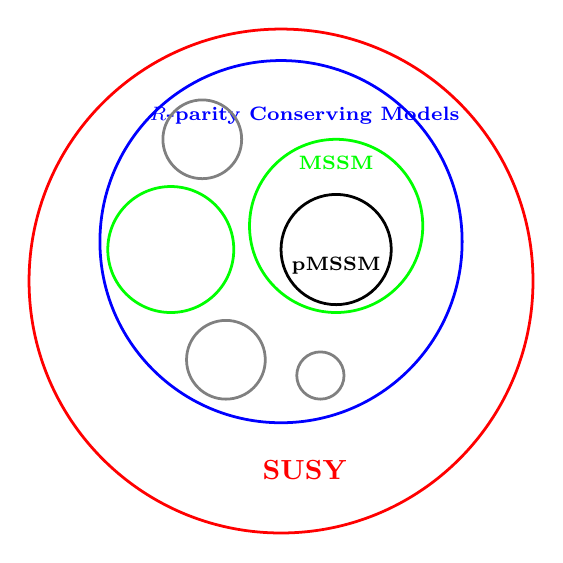
\begin{tikzpicture}
        \draw[draw=red, line width=1] (4.9,2.4) arc(0:360:3.2 and 3.2);
        \node[align=center,red,font={\bfseries}] at (2,0) {SUSY};
        
        \draw[draw=blue, line width=1] (4,2.9) arc(0:360:2.3 and 2.3);
        \node[align=center,blue,font={\scriptsize\bfseries}] at (2.,4.5) {$R$-parity Conserving Models};%N=1};

        \draw[draw=green, line width=1] (3.5,3.1) arc(0:360:1.1 and 1.1);
        \node[align=center,green,font={\scriptsize\bfseries}] at (2.4,3.9) {MSSM};
        \draw[draw=green, line width=1] (1.1,2.8) arc(0:360:0.8 and 0.8);
        \node[align=center,green,font={\scriptsize\bfseries}] at (0.4,2.6) {};%NMSSM};

        \draw[draw=black, line width=1] (3.1,2.8) arc(0:360:0.7 and 0.7);
        \node[align=center,black,font={\scriptsize\bfseries}] at (2.4,2.6) {pMSSM};
        \draw[draw=gray, line width=1] (1.5,1.4) arc(0:360:0.5 and 0.5);
        \draw[draw=gray, line width=1] (2.5,1.2) arc(0:360:0.3 and 0.3);
        \draw[draw=gray, line width=1] (1.2,4.2) arc(0:360:0.5 and 0.5);

        %\node[black,font={\tiny}] at (2,-1.3) {T. Rizzo, SLAC Summer Institute 2012};
          \end{tikzpicture} 
          
\caption[Illustration of the pMSSM as a subset of SUSY theories]{An illustration of the pMSSM as a subset of the larger MSSM, both under the larger umbrella of SUSY theories (figure based off of \cite{rizzossi2012}).}% with one SUSY transformation, N=1.} 
\label{fig:pmssm}
\end{figure}
%
%%\subsection{Mass Spectrum}
%%
%%In the MSSM there are two complex Higgs doublets rather than just one as in the SM.  Each get their own VEV as $\langle H_{u} \rangle = v_{u}$ and $\langle H_{d} \rangle = v_{d}$.  This are related to the mass of the {\Zboson} boson and electroweak gauge couplings as:
%%
%%\begin{equation}
%%v_u^2 + v_d^2 = v^2 = \frac{2m_{\Zboson}^2}{(g^2+g^{'2})} \approx (246 \mathrm{GeV})^2
%%\end{equation}
%%
%%with the ratio between the two \gls{vev}:
%%
%%\begin{equation}
%%\tan \beta \equiv \frac{v_u}{v_d}
%%\end{equation}
%%%\frac{\pi}{2}$.
%%
%%where both $v_u$ and $v_d$ are real and positive, and the value of $\tan \beta$ is not fixed by experiments but depends on Lagrangian parameters but must be $0 < \tan \beta < \frac{\pi}{2}$.  \\
%%
%%The Higgs scalar fields in the MSSM consist of eight real scalar degrees of freedom.  After electroweak symmetry breaking three of these are the Nambu-Goldstone bosons, $G^{0}$ and $G^{\pm}$, that become longitudinal modes of the $Z^0$ and $W^{\pm}$ bosons.  The other five degrees Higgs scalar mass eigenstates include two CP-even neutral scalars, $h^0$ and $H^0$, one CP-odd neutral scalar $A^0$, one charge +1 $H^+$, and one which is its conjugate $H^-$. The discovered $\sim 125$ GeV Higgs is usually assumed to be the lighter $h^0$. \\
%
%%%Electrowinos  
%%
%%  The exact mixing varies from model to model, so the mass and charge are the focus of experimental searches.  The lightest neutralino is assumed to be the lightest supersymmetric partner (LSP), unless there is a lighter gravitino or unless $R$-parity is not conserved, and is therefore the only particle in the MSSM that makes a good dark matter candidate.  \\
%%
%%% gluino
%%
%%The gluino is a color octet fermion and so cannot mix with any other particle in the MSSM. Its mass parameter, $M_{3}$ is related to the bino and wino mass parameters, $M_{1}$ and $M_{2}$ as $M_{3}:M_{2}:M_{1} \approx 6:2:1$ (following MSUGRA or GMSB boundary conditions) so the gluino is expected to be much heavier than the neutralinos and charginos.  \\
%%
%%% sfermions
%%
%%The squarks in the first and second families are nearly degenerate and are much heavier than the sleptons due to large radiative corrections from loops with the gluino, and cannot be much lighter than the mass of the gluino.  Additionally, left-handed sfermions are heavier than right-handed sfermions due to effects from the renormalization group.  The third family sfermions are most likely the lightest sfermions due to contributions from their renormalization group equations. \\
%
%%Potentially dangerous flavor-changing and CP-violating effects in the MSSM can be avoided if SUSY breaking is universal.  In the case where the squark and slepton squared-mass mixing angles are flavor-blind, and each proportional to the 3x3 identity matrix in family space, the squark and slepton mixing angles are trivial and SUSY contributions to flavor changing currents are very small.  Additionally, assuming the scalar couplings are proportional to the corresponding Yukawa coupling matrix ensures that only squarks and sleptons of the third family can have large scalar couplings.  Furthermore, large CP-violating effects can be avoided by assuming soft parameters do not introduce new complex phases.  These conditions make up a weak version of the soft supersymmetry-breaking universality hypothesis and has fewer parameters than the general case.  There are several alternatives to the universality hypothesis but add complexity or require very heavy masses. \\
%
%%\begin{figure}[tbh]
%%	\centering
%%	\includegraphics[width=.5\textwidth,trim={0 0 0 0},clip]{massspectrum}
%%	\caption{A possible mass spectrum for the MSSM.  This is one particular model for GMSB; different models vary greatly, including in mass scales, which is not shown.  \cite{susyprimer} \color{red}{Replace with higher resolution image.  Add other possible spectra?} }
%%	\label{fig:massspect}
%%\end{figure}
%% squark decays
%
%%The decay of a squark to a quark and gluino will dominate if kinematically allowed because it has QCD strength.  Otherwise squarks can decay to a quark and neutralino or chargino, and the decay to a quark and LSP is kinematically favored and can dominate for right-handed squarks if the LSP is mostly bino.  Left-handed squarks may prefer decaying to heavier neutralinos and charginos because the coupling to winos is stronger than binos.  \\
%
%
%\section{Simplified Models}
%
%While a new model of physics can involve many new and complex particles and interactions, simplified models are designed to only involve a few new particles and interactions.  These can be limits of more complex scenarios but with new particles integrated out and can be described by a few parameters related to collider physics, such as particle mass, production cross-sections, and branching fraction.  Figure \ref{fig:stopSimple} shows the simplified model in this search with a gray blob after the proton collision but before the stop production that represents model-specific physics that is integrated out for the simplified model.  This helps to avoid some of the limitations of model-dependent searches and sensitivity to new physics can be presented of a function of these few parameters and over full ranges of new particle masses.  The primary application for simplified model results are to identify the boundaries of search sensitivity, describing new physics signals, and deriving limits on more general models. \\
%
%In this search with $R$-parity conserving models the stop cross section is mostly decoupled from the model parameters\cite{Beenakker:1997ut, Beenakker:2010nq, Beenakker:2011fu, Borschensky:2014cia}.  The stop decay depends on the left- and right-handed stop mixing, the mass of the stop, and the mixing parameters of the charginos and neutralinos.  
%
%\begin{figure}[tbh]
%	\centering
%	\includegraphics[width=.4\textwidth,trim={0 0 0 0},clip]{stst-ttN1N1.pdf}
%	\caption{\label{fig:stopSimple}{Simplified models of stop pair production.  The gray blob after the proton collision represents a black box with potentially complex physics, which is integrated out.}}
%\end{figure}
%
%
%
%\subsection{Search for Direct Pair-Produced Stops}
%
%Because the stop quark is the lightest sfermion while also having the largest impact on fixing the hierarchy problem, searching for the stop is well-motivated.  Introducing $R$-parity preserves baryon and lepton number conservation while also providing a candidate for dark matter, which means that stop quarks are produced in pairs.  
%
%
%
%
%
%%As a scalar particle, the Higgs mass correction goes as:
% %Because the top quark is so much more massive than other fundamental particles (nearly 40 times heavier than the next heaviest fermion) and because of the large top Yukawa coupling,  its mass essentially sets the mass correction for the higgs. 
%
%%\begin{equation}
%%\feynmandiagram [inline=(a.base), layered layout, horizontal=b to c]
%%{ 
%%	a -- [scalar] b 
%%	-- [fermion, half left, looseness=1.6, edge label=\(t\)] c 
%%	-- [fermion, half left, looseness=1.6] b,
%%	c -- [scalar] d,
%%};
%%= -\frac{6y_t^2}{16\pi^2}\Lambda_{\mathrm{UV}}^2
%%\label{eq:toploop}
%%\end{equation}
%

\chapter{Experimental Setup}
\label{ch:experiment}

This chapter describes the experimental apparatus that was used in the search: the machine that produces high energy collisions, the Large Hadron Collider (LHC), and the detector used to measure particle properties, ATLAS.

\section{Proton-proton Collisions at the Large Hadron Collider}
%LHC paper
The LHC is the world's largest particle accelerator.  The tunnel, originally used for the CERN Large Electron-Positron Collider (LEP) and reused for the existing structure to avoid building a new tunnel, is 26.7 km in circumference and lies between 45-170 m underground in order to reduce cosmic radiation backgrounds.  The LHC accelerates protons clockwise and counterclockwise around the ring, currently with each beam having an energy of 6.5 TeV, which corresponds to more than 99.9999\% of the speed of light.  The advantage of a collider over, for instance, a fixed target accelerator, is that the center of mass energy scales as $E_{CM} = 2E_{L}$, where $E_{L}$ is the energy of each beam, as opposed to a fixed target accelerator where the center of mass energy scales as $E_{CM}=\sqrt{E_{L}}$ due to the necessary contribution to the kinetic energy of the target.  Therefore the center of mass energy of the LHC is currently 13 TeV.\\

While a lepton accelerator would produce cleaner collisions, protons are used to reduce the energy loss from synchrotron radiation, which scales as the fourth power of the particle mass.  Also proton-proton collisions are used instead of proton-antiproton, as was the case of the Tevatron at Fermilab, due to the fact that the time required to produce antiprotons would limit luminosity.  This has the effect that nearly all the produced particles stem from gluon-gluon fusion instead of quark-antiquark annihilation.  The LHC also produces heavy ion collisions.\\

It takes several separate machines to accelerate protons to this energy and superconducting magnets are used to focus, steer, and accelerate the protons around the ring.  Four main detectors study the collisions; two general purpose detectors, ATLAS and CMS, and two specialty detectors, ALICE (primarily studying heavy ion physics) and LHCb (primarily studying b-quark physics). \\%references for each detector?



\subsection{Accelerator Complex}

Several steps are required to accelerate protons to the energy of the LHC.  The protons begin as hydrogen gas (which is composed of a proton with an electron) from bottled hydrogen and is placed into an electric field to strip away the electrons, leaving the positively charged protons.  From here the protons are injected into the Linac2, a linear accelerator where they are accelerated to 50 MeV and injected into the Proton Synchotron Booster and accelerated to 1.4 GeV.  The Proton Synchrotron then accelerates the protons to 25 GeV, then the Super Proton Synchrotron accelerates them to 450 GeV.  The beam is finally injected into the LHC, where it is accelerated to its final momenta.  This is performed using 16 radiofrequency (RF) cavity systems which operate at 400 MHz.  The components of the accelerator complex can be seen in Figure \ref{fig:lhcMachine}.  \\

\begin{figure}[h!]
  \centering
	\includegraphics[width=0.8\textwidth]{./figures/lhcMachine.pdf}
\caption{\label{fig:lhcMachine}{ The LHC accelerator complex\cite{LHC}. }}
\end{figure}

The RF cavities generate an oscillating voltage such that the particles are accelerated at the gap, and since the particle must always be accelerated at the gap the RF frequency must be an integer multiple of the revolution frequency.  The segments of the circumference of the beam centered on this point are called buckets.  Particles that are synchronized with the RF frequency are called synchronous particles and other particles will oscillate around these particles.  Therefore particles get clumped around synchronous particles (rather than a uniform spread) in a bunch that is contained in an RF bucket.  Because of this the LHC can accelerate a beam made up of 35640 bunches.  This is complicated because the PS and SPS are also synchrotrons, and the PS is actually responsible for providing bunch packets with the 25 ns spacing that the LHC uses.  Also, the buckets can be full of protons or be empty; the purpose of empty buckets is to accommodate the time required to dump the beam.  The configuration also determines where the beams cross and collide, which corresponds to different detectors.   \\ %include table 4.1?

The quality of the beam is important, which is expressed in part by beam emittance and beta.  Beam emittance refers to the distance a beam is confined to and how similar the particles are in momenta (a small beam emittance corresponds to a closer grouping with the same momentum).  A small emittance increases the luminosity by increasing the likelihood of interaction.  Beta is determined by the cross section of the bunch and the emittance, so a low beta indicates a more squeezed beam.\\


\subsection{LHC Magnets}

The protons in the beam are steered using 1.232 dipole magnets, each of which are 14.3 meters in length, producing up to 8.4 Tesla magnetic fields.  This is achieved using superconducting niobium-titanium (NbTi) Rutherford cables operating at 1.9K with about 11,800 amperes of current.  \\

Because the beams are charged, they will diverge if not focused.  Additionally, 392 quadrupole magnets, each between 5-7 meters in length, and each with two apertures, one for each direction, are used to focus the beam.  One set of quadrupole magnets squeezes the beam horizontally (QF), another set vertically (QD). \\%858 quadrupole magnets total?

\subsection{Luminosity}

Luminosity is defined by the number of collisions produced in a detector per square centimeter per second.  This can be determined by the square of the number of particles in a bunch (since each can collide with any in another bunch), the time between bunches, and the cross section of a bunch.  This can also be expressed as a function of the beam emittance and beta, as described above.  The integrated luminosity, which is the total delivered luminosity, is shown in Figure \ref{fig:intLum} for 2012-2017.\\

\begin{figure}[h!]
  \centering
	\includegraphics[width=0.8\textwidth]{./intlumivsyear.eps}
\caption{\label{fig:intLum}{ Integrated luminosity for individual years of running. }} %luminosity twiki
\end{figure}

%ATLAS paper

\subsection{Pileup}

While increasing luminosity is necessary and beneficial for data collection, it corresponds to a major challenge as well; an increase in the number of interactions per bunch crossing, or pileup $(\langle \mu \rangle)$.  Most interactions are not the hard-scatter events that create potentially interesting physics events, but softer collisions that are not of interest and create noise while raising trigger rates.  It's important to reduce plieup as much as possible. Figure \ref{fig:mu} shows the mean number of interactions per crossing for the years 2015-2017 and can be seen that the number has increased each year. \\% and techniques to mitigate it have been and are being developed.

\begin{figure}[h!]
  \centering
	\includegraphics[width=0.8\textwidth]{./mu_2015_2017.pdf}
\caption{\label{fig:mu}{ Pileup during data taking in 2015-2017. }} %luminosity twiki
\end{figure}

\section{Overview of the ATLAS Detector}
%ATLAS paper
The ATLAS detector, as shown in Figure \ref{fig:atlas}, is a general-purpose detector and is the largest detector ever built at 46 meters in length and weighing in at 7000 tons.  Its muon system magnets are toroidal in shape, and is perhaps best described as a toroidal LHC apparatus.  It's nominally forward-backward symmetric with regards to the interaction point, covering nearly the complete solid angle.  It is a general purpose detector that can detect a variety of new physics while also improving Standard Model measurements, and, along with CMS, discovered the Higgs Boson in 2012.  \\

ATLAS uses a variety of technologies to provide accurate and precise measurements of particle trajectories and momenta and consists of three primary subdetectors: the Inner Detector, which measures the paths of charged particles, calorimeters, which measures momenta of charged and neutral particles, and the muon system, which measures the paths of high energy muons.   Figure \ref{fig:energyDeposits} shows in what subsystem particles deposit energy or leave tracks.  Additionally, the trigger system reduces the event rate from 40 MHz to an order of a kHz to make data collection feasible.  A network of computer systems, both on site and off site, allows for data handling and storage as well as supporting analyses.\\

\begin{figure}[h!]
  \centering
	\includegraphics[width=0.8\textwidth]{./figures/energyDeposits}
\caption{\label{fig:energyDeposits}{ Cut-away view of ATLAS showing where particles deposit tracks and energy. }} %luminosity twiki
\end{figure}


\begin{figure}[h!]
  \centering
	\includegraphics[width=1.\textwidth]{./figures/atlas.pdf}
\caption{\label{fig:atlas}{ Cut-away view of the ATLAS detector and its subsystems.  Illustrations of people are included to provide a sense of scale. }} %luminosity twiki
\end{figure}


\subsection{Coordinate System and Common Variables}

%ATLAS paper
ATLAS uses a right-handed coordinate system where the interaction point is the origin of the coordinate system.  The beam direction defines the z-axis and the x-y plane is transverse to the z-axis.  Positive x points toward the center of the LHC ring and positive y points upwards.  Side-A of the detector is defined as positive z and side-C as negative.  Azimuthal angle $\phi$ is measured around the beam axis, and the polar angle $\theta$ defined as the angle from the beam axis.  Pseudorapidity, $\eta$, is defined as $\eta = -ln[tan(\theta/2)]$ and rapidity, y, as $y=\frac{1}{2} ln(\frac{E+p_{z}}{E-p_{z}})$ in the case of massive objects.  The transverse momentum, \pt\,  the transverse energy, $E_{\mathrm{T}}$, and the missing transverse momentum (denoted as energy), $E_{\mathrm{T}}^{miss}$, are defined in the x-y plane.  The $E_{\mathrm{T}}^{miss}$ is limited to the x-y axis because momenta of colliding particles (such as gluons) in the z direction is unknown.  Finally, the distance $\Delta R$ is defined as $\Delta R = \sqrt{\Delta\eta^{2} + \Delta\phi^{2}}$.\\

\subsection{Magnet System}

ATLAS has two magnet systems of note, the solenoid magnet and toroid magnets.\\

A thin superconducting solenoid magnet surrounds the inner detector and creates a 2T field that makes the tracking of charged particles possible.  \\

The toroid system consists of two parts, the endcap and barrel magnets as shown in Figure \ref{fig:atlasToroids}.  The magnets consists of eight coils, symmetrically arranged around the beam axis and radially assembled, weighing 830 tons.  The peak field is of the barrel magnets 3.9T and 4.1T for the endcap magnets.  This strong magnetic field permits tracking high energy muons to determine momentum.\\

\begin{figure}[h!]
  \centering
	\includegraphics[width=0.8\textwidth]{./figures/toroidMagnets.pdf}
\caption{\label{fig:atlasToroids}{ Layout of the ATLAS toroid magnets. }} %luminosity twiki
\end{figure}

\subsection{Inner Detector}

The inner detector, which sits inside the 2T solenoid magnet, is used to reconstruct tracks that charged particles make as they bend in the magnetic field.  It provides hermetic coverage and pattern recognition, extending to $\eta=2.5$, and also provides momentum resolution and both primary and secondary vertex measurement.  Secondary vertices are important to identify and measure particles with delayed decays, such as bottom quarks, charm quarks, and tau leptons.  \\

The inner detector consists of several subsystems.  Going from innermost to outermost of the beam, they are the insertable b-layer (IBL, the newest addition, added during Long Shutdown I), silicon pixel detectors, and the transition radiation tracker.  This can be seen in Figure \ref{fig:innerDetector}.\\

The IBL was added to be closer to the IP and thus improve vertexing, and involved adding a smaller beam pipe.  It uses a combination of planar technology, the same as the silicon pixel layers, and 3D technology, where the electronics pass through the bulk of the sensors in addition to lying on the surface.  The 3D technology covers the outermost 25\% of the IBL to improve resolution in the forward regions. \\ % http://iopscience.iop.org/article/10.1088/1748-0221/9/02/C02018/pdf

The silicon pixel detector consists of three pixel layers.  The pixel sensor is made by implanting high positive and negative dose regions on each side of a wafer, so when a charged particle passes through the wafer an electric current passes through it.  The design also ensures single pixel isolation and minimizes leakage current.  The SCT can provide up to 4 additional measurement points, so these layers provide good tracking information.  \\%http://iopscience.iop.org/article/10.1088/1748-0221/3/07/P07007/pdf

The transition radiation tracker (TRT) consists of 73 straw planes in the barrel and 160 in the endcap, extending to $|\eta|=2.0$.  The detector exploits the fact that charged particles emit electromagnetic radiation with moving from one medium to another, in this case carbon dioxide and polypropylene.  The energy loss depends on the mass of the particle, so lighter particles emit more of their energy.  Emitted EM radiation interacts with the gases inside a tube to increase the current when a charged particle passes though.  This can distinguish between, for instance, electrons and pions.  While the resolution of the TRT is less than the silicon wafers, extending silicon wafers out to the endpoint of the TRT is cost prohibitive.  \\

\begin{figure}[h!]
  \centering
	\includegraphics[width=0.8\textwidth]{./innerDetectorIBL.pdf}
\caption{\label{fig:innerDetector}{ Cut-away view of the ATLAS inner detector\cite{IBL}. }} %luminosity twiki
\end{figure}

\subsection{Calorimeters}  \label{sec:calorimeters}%into to next section

Unlike the ID, which changes the path of charged particles to provide tracking information, the calorimeters absorb both charged and neutral particles to measure their energy.  The exception to this is muons, which pass through the calorimeters, as well as neutrinos which pass through the entire detector without detection.  This can be done with a homogeneous material, like a scintillator, or with separate layers of absorber and detector material, called a sampling calorimeter.  This is the case with the ATLAS liquid argon (LAr) calorimeter, in which lead (absorber) and liquid argon (detector) is arranged in an accordion shape with copper-tungsten sensors as can be seen in \ref{fig:larLayout}.  Lead is chosen because its density increases the probability of interaction with the particles, and argon is chosen because it is radiation hard, stable, and affordable.  The particle interacts with the absorber material to generate secondary particles.  This in turn creates cascades of particles, the energy of which is measured from ionizations in the detector regions.  This aids in measuring neutral particles, the energy of which is measured by the secondary particles they create.  The absorptive power is also statistical as a Poisson distribution so precision depends on $\frac{\Delta E}{E}$ and varies like $\sqrt{E}$ while spectrometers vary as $E^{2}$.  There is also a fast response, which aides in triggering.  However, the measured energy is limited to a few tens of percents of the signal, so statistics has a large effect.  The radiation length ($\chi_{0}$) of a description of a material where, by passing through it, 1/e of a particle's energy is lost to bremsstrahlung (also 7/9 of the mean free path for photon pair production).  There are at least 25 radiation lengths through any path in the calorimeter.  The number of radiation lengths through different portions of the calorimeter is shown in Figure \ref{fig:radLengths}.  The LAr calorimeter primarily measures the energy of electrons and photons.\\

\begin{figure}[h!]
  \centering
	\includegraphics[trim=0cm 1cm 0cm 0cm,clip, width=1\textwidth]{./figures/calorimeters.pdf}
\caption{\label{fig:calorimeters}{ Cut-away view of the ATLAS calorimeters\cite{DetectorPaper:2008}. }} %luminosity twiki
\end{figure}

\begin{figure}[h!]
  \centering
	\includegraphics[width=1\textwidth]{./figures/RadLegths.pdf}
\caption{\label{fig:radLengths}{ Number of radiation lengths ($\chi_{0}$) as a function of $\eta$. }} %luminosity twiki
\end{figure}


Hadrons can only be measured by hadron-nucleon interactions, which is characterized by the mean free path of the hadron, its nuclear interaction length.  While the EM calorimeter is adequate for absorbing electrons and photons, it is only about 2 nuclear interaction lengths to measure the energy of hadrons.  Beyond the liquid argon calorimeter is the hadronic calorimeter, which adds 9 intreraction lengths.  The number of interaction lengths through different parts of the hadronic calorimeters is shown in Figure \ref{fig:interactionLengths}.  The hadronic calorimeter is another sampling calorimeter in which steel is used as absorber and scintillating tiles sandwiched between the steel layers measure the deposited energy.  This choice in technology was partly for cost savings as this is a large subdetector, providing coverage up to $|\eta|<1.7$ and radially extending from 2.28 m to 4.25 m.  \\

\begin{figure}[h!]
  \centering
	\includegraphics[width=0.8\textwidth]{./figures/interactionLengths.pdf}
\caption{\label{fig:interactionLengths}{ Number of interaction lengths as a function of $\eta$. }} %luminosity twiki
\end{figure}

\section{Liquid Argon Calorimetry at ATLAS}

As discussed previously, the Liquid Argon calorimeter is a sampling calorimeter capable of absorbing and measuring the energy of charged and neutral particles.  The LAr calorimeter covers the pseudorapidity range $|\eta| < 3.2$.  The hadronic calorimeter is comprised of a scintillator-tile calorimeter, separated into a large barrel and two smaller extended barrel cylinders on each side of the central barrel and covers the pseudorapidity range $|\eta| < 1.7$.  The endcaps, with $|\eta| > 1.5$ also use LAr calorimetry and extend to $\eta = 3.2$.  The LAr forward calorimeters provide EM and hadronic measurements and extend to $\eta = 4.9$.  Because of the complexity of the arrangement, there are some gaps in the coverage; otherwise, coverage is nearly hermetic.  \\

A aspect to the LAr calorimeter is that it must be kept very cold to operate, so is housed in a cryostat operated at 89K, which contributes to dead material.  In order to reduce the total amount of dead material the LAr calorimeter shares the cryostat and vacuum vessel with the solenoid magnet.  \\

The LAr calorimeter typically operates at a 2000V, with some variance, to create a particle avalanche when a charged particle ionizes the liquid argon.  There is a presampler layer in the barrel region, which corrects for energy loss in material upstream of the calorimeter, followed by three additional layers, which sum together to form a Trigger Tower, which are analog sums of energy deposits contained in an area of $\Delta\eta \times \Delta\phi$ = $0.1 \times 0.1$ across longitudinal layers of the calorimeters.\\

\begin{figure}[h!]
  \centering
	\includegraphics[width=0.8\textwidth]{./figures/larLayers.pdf}
\caption{\label{fig:larLayout}{ An illustration of a LAr calorimeter module in the barrel region which shows the accordion structure of the absorbers and the geometry of each section and a Trigger Tower\cite{LArTDR}  }} %LAr TDR
\end{figure}


\subsection{Signal Propagation}
%LAr tdr (1997)
The drift time in the LAr calorimeter is 400-600 ns, compared to the 25 ns bunch-crossing time.  To prevent signal overlapping, an RC-CR\textsuperscript{2} shaping with a time constant of 20 ns is applied to analog signals, which minimizes sensitivity to pileup and electronic noise and results in a 100 ns positive pulse and 400 ns negative lobe as shown in Figure \ref{fig:larPulse}.  This pulse shape gives an integral of 0, although it is unlikely that any sampled value is exactly 0.  The most likely measured value is called the pedestal.  The most significant quantity for the scale of the signal is the peak current in a readout cell corresponding to an energy deposit.  Both the pileup and the mean energy of a calorimeter cell depend on how signals are treated.\\

\begin{figure}[h!]
  \centering
	\includegraphics[width=0.6\textwidth]{./LArPulse.pdf}
\caption{\label{fig:larPulse}{ Signal shape before shaping (triangle) and after shaping (curved with dots).  The dots are positions of successive bunch crossings\cite{DetectorPaper:2008}. }} 
\end{figure}


Since the calorimeters use warm preamplifiers (with exception to the HEC) for long term reliability, the shaping stage is designed to handle both pileup and thermal noise.  It also must cover a dynamic range in excess of 17 bits, so the range is split by three linear output ranges with gains of 1, 10, and 100.  This means that necessary range can be covered by the 12 bit system downstream of the shaper.  The shaped signals are sampled and stored in analog form by switched-capacitor array (SCA) analog pipeline chips.  \\

After the front-end board (FEB), off-detector boards perform digital filtering used to extract information from five samples around the peak of the pulse shape.  Analog sums are performed in steps due to the large number of channels on the shaper chip, the FEB, and on designated boards in front-end crates and used to form trigger towers.  Figure \ref{fig:sigProp} shows the signal path in the LAr electronics.  \\

\begin{figure}[h!]
  \centering
	\includegraphics[width=0.8\textwidth]{./signalProp}
\caption{\label{fig:sigProp}{ Signal propagation through the LAr electronics\cite{larPerf}. }} %LAr TDR
\end{figure}

\subsection{Calibration}

In order to properly measure the energy deposited in a cell, the calorimeters must be properly calibrated.  The conversion of signal Analog to Digital Converter (ADC) samples to raw energy depends on the conversion of ADC to Digital Analog Converter (DAC), called the Ramps, the Optimal Filtering Coefficients, which use a noise autocorrelation function of the samples (the ratio of thermal to pileup noise amplitudes) to maximize the signal/noise ratio and determine the time origin and amplitude of the signal, and the Pedestals as described previously. \\


In order to calibrate these items:
\begin{itemize}
	\item Pedestal, noise, and noise autocorrelation: FEBs are read with no input signal and performed separately for each gain
	\item Ramp: Scan input current and fit DAC vs. ADC curve
	\item Delay: All cells pulsed with a known current signal and a delay between calibration pulses and DAQ introduced - this allows for full calibration curve to be reconstructed
\end{itemize}

Once these values are properly set one can go find the energy in a cell with:

\begin{equation}
	E=\Sigma F_{j} (\Sigma a_{i}(ADC_{i} - P))^{j}
\end{equation}

where E is the energy, $F_{j}$ are the ramps, $a_{i}$ are the OFCs, $ADC_{i}$ are the raw samples and $P$ are the pedestals.  \\

In order to detect the Higgs boson, the uncertainty must be small, especially in channels that led to the Higgs discovery, $H \rightarrow \gamma \gamma$ and and $H \rightarrow 4l$.  The low uncertainty for electron $p_{T}$ can be seen in Figure \ref{fig:euncertainty} and the uncertainty in the four lepton channel is 0.7\% of the overall 8.0\%\cite{HiggsAtlas}. \\

\begin{figure}[h!]
  \centering
	\includegraphics[width=1\textwidth]{./eUncertainty.pdf}
\caption{\label{fig:euncertainty}{Electron uncertainty as a function of $p_{T}$ (left) and $\eta$ (right)\cite{eUncertaintyPaper}.  The low uncertainty leads to more precise measurements on important quantities, such as the Higgs mass.}} 
\end{figure}

Calibration is also important for the missing energy trigger.  Missing energy, an imbalance of momentum of detected particles, is an indication of new physics as there could be new particles that pass through the detector without interacting with it.  Mis-measured energy can give a false positive for a new particle, so any uncertainty pushes up the quantity of missing energy that can be triggered on with reasonable rates.  Therefore the uncertainty on measured momentum must be minimized.  This is discussed further in section \ref{sec:met}.

\subsection{Forward Detectors}

There are additional calorimeters in the forward region that deal with high particle flux: two for EM showers, the electromagnetic end-cap calorimeter (EMEC) and the forward calorimeter (FCal), and one for hadronic showers, the hadronic end-cap calorimeter (HEC).  All these use liquid argon as the active material, including the HEC as scintillating tiles would degrade in the high particle flux.  The absorber material used have shorter radiation lengths and nuclear interaction lengths; lead is used for the EMEC and FCal and copper-tungsten is used in the HEC. \\

There are two forward detectors that measure luminosity, LUCID (LUminosity measurement using Cerenkov Integrating Detector), ALFA (Absolute Luminosity For ATLAS), and ZDC (Zero-Degree Calorimeter).  LUCID detects inelastic p-p scattering in the forward region and is the main luminosity monitor for ATLAS.  ALFA is located $\pm$240m down the beam line and contains fiber trackers inside Roman pots, designed to be as close as 1mm to the beam.  ZDC is used with heavy-ion collisions and is located $\pm$140m down the beam pipe, just before the single beam pipe separates into two, and consists of alternating quartz rods and tungsten plates to measure neutral particles to measure centrality of heavy-ion collisions.\\



%Bill Cleland's paper

%To determine the amplitude and timing of samples one uses optimal filtering.  This uses the autocorrelation function of the samples, which is a function of the ratio of thermal to pileup noise amplitudes, to maximize the signal/noise ratio to determine the time origin and amplitude of the signal.  

% Overview of LAr, operations, 


\subsection{Muon System}

The outermost layer of the detector is the muon spectrometer, which measures the momentum of muons whose path bends in the strong magnetic field from the toroid magnets it is emerged in.  The central region, $|\eta|<2.7$ has three layers of Monitored Drift Tubes (MDTs), for tracking, and Resistive Plate Chambers (RPCs), for the trigger system.  In forward regions, Cathode Strip Chambers (CSCs) are multiwire proportional chambers and can handle high rates and harsh conditions.  Thin Gap Chambers (TGCs) are used in the end-cap regions.  Muons will usually hit three layers to provide tracking and momentum information.  Figure \ref{fig:muonCutAway} shows the ATLAS muon system.  \\

\begin{figure}[h!]
  \centering
	\includegraphics[trim=0cm 1cm 0cm 0cm,clip, width=0.8\textwidth]{./figures/muonSystem.pdf}
\caption{\label{fig:muonCutAway}{ Cut-away view of ATLAS Muon System\cite{DetectorPaper:2008}. }} %luminosity twiki
\end{figure}

%
%History (luminosity and plots, pileup)
%\subsection{Trigger and Data Acquisition} %intro for next section

  


\section{The ATLAS Trigger System}

The ATLAS trigger system has the job of reducing the enormous quantity of data collected by the detector and reducing the rate to a reasonable one.  The LHC machine has a crossing rate of 40 MHz and data on the order of a kHz can be read out.  To do this the trigger uses a hardware trigger (Level 1, or L1) followed by software-level triggers (the High Level Trigger, or HLT).  \\

The hardware trigger uses fast algorithms with subsets of detector information to reduce the rate to 75 kHz.  The L1Calo trigger uses the calorimeter systems for electrons, photons, hadrons, jets, and $E_{\mathrm{T}}^{miss}$.  The L1Muon trigger uses muon information from the muon system.  The results from the L1 systems are passed to the central trigger processor, which implements a trigger menu made of combinations of trigger selections.    The L1 systems identify regions of interest (RoI) defined by detector geometry and criteria passed, which are passed to the HLT.  The decision time is 25 $\mu$s. \\

The Level 2 (L2) trigger, part of the HLT, uses RoIs from the L1 trigger along with full detector granularity to make selections and are designed to reduce the rate to about 3.5kHz in 40 ms.  Finally, the Event Filter reduces the rate to about 1-2 kHz using offline analysis procedures in about 4 seconds.  \\



%%%%%%%%%%%%%%%%%%%%%%%%%
\section{Calorimeter Trigger Phase I Upgrades}
%gFEX FDR
At the end of Run 2 the LHC will have delivered an impressive 150 fb\textsuperscript{-1} of data.  However, if the LHC continues to run with the same luminosity as in Run 2 the statical gain would be marginal.  Therefore, an increase in instantaneous luminosity is planned during Long-Shutdown 2 (LS2), scheduled for the end of 2019 and taking 24 months.  During this time the Phase-I upgrade will take place.  This includes major upgrades; at the accelerator complex, Linac2 will be replaced by Linac4, which is expected to double the brightness of the beam from the PSB, reducing the beam emittance with smaller $\beta$ functions.  This will increase the luminosity from the current $1.37\times10^{34}$cm\textsuperscript{-2}s\textsuperscript{-1} to $2-3\times10^{34}$cm\textsuperscript{-2}s\textsuperscript{-1}.  During the Run 3 an estimated 300 fb\textsuperscript{-1} will be delivered. \\ %Afterwards a longer future shutdown, LS3, is planned to upgrade the LHC to the High Luminosity LHC (HL-LHC), and is discussed in the next section. \\

The instantaneous luminosity planned for Run 3 corresponds to 55-80 interactions per bunch crossing (pileup) with a 25 ns bunch spacing.  Maintaining an optimal trigger system in these conditions requires a trigger electronics upgrade, including improvements in object energy resolution and more advanced algorithms to maintain a high trigger acceptance and rate for L1Calo objects, while also triggering on events with boosted hadronically decaying bosons.  The LAr calorimeter will increase in granularity by an order of magnitude to accomplish this. \\

%LAr Phase-I TDR
The current calorimeter trigger information consists of Trigger Towers; during the Phase-I upgrade the granularity will be increased by using Super Cells, which include information from each layer as well as providing finer segmentation within the middle layers as shown in Figure \ref{fig:superCell}.  The presampler and the last layer will keep the $\Delta\eta \times \Delta\phi$ = 0.1$\times$0.1 geometry while the front and middle layers will increase in granularity to $\Delta\eta \times \Delta\phi$ = 0.025$\times$0.1.  This means an increase in granularity by a factor of 10 depending on the part of the barrel and improves energy resolution and efficiency for selecting electrons, photons, $\tau$ leptons, jets, and $E_{\mathrm{T}}^{\mathrm{miss}}$ while also improving discrimination against backgrounds and fakes in high pileup conditions.  \\

Additionally, new LAr Trigger Digitizer Boards (LTDB) will be installed on the Front-End crates.  These will both digitize high-granularity information from the calorimeters and also create analog sums to maintain a functional legacy system.  \\

\begin{figure}[h!]
  \centering
	\includegraphics[width=0.8\textwidth]{./figures/superCell.pdf}
\caption{\label{fig:superCell}{ A sample event of a 70 GeV electron as seen by the current L1Calo Trigger, with all cells summed into a Trigger Tower (a) and after the Phase I upgrade with Super Cells (b)\cite{LArPhaseITDR}. }} %LAr TDR  DONE
\end{figure}


%gFEX fdr
After digitization the LTDB transfers calorimeter signals to the LATOME (LAr Trigger prOcessing MEzzanine) cards in the off-detector LAr Digital Processing System (LDPS), each of which uses a filtering algorithm on an FPGA to reconstruct the transverse energy of the Super Cells every 25 ns and identifies the related bunch-crossing (BCID).  The LATOME then transmits information to the new feature extraction processors (FEXs) that will implement sophisticated object identification algorithms.  These include the eFEX, jFEX, and gFEX.  The eFEX receives full super cell information, and the jFEX receives $\Delta\eta \times \Delta\phi$ = 0.1$\times$0.1 super cell energy sums. Figure \ref{fig:l1calo} shows the updated L1Calo system.  \\%, and the gFEX receives $\Delta\eta \times \Delta\phi$ = 0.2 $\times$ 0.2 super cell energy sums. % Output data from the FEXs are processed and buffered by LDPS after an L1 trigger acceptance (L1A) and are routed toe the Front End Link EXchange (FELIX), which interfaces the ATLAS sub-detectors to the data acquisition system.  The FELIX also allows the system to handle bi-directional low-latency channels by routing data to and from multiple Gigabit Bidirectional Trigger and Data Links (GBTs) by the way of a high-performance general purpose network.

\begin{figure}[h!]
  \centering
	\includegraphics[width=0.8\textwidth]{./phaseIelectronics.pdf}
\caption{\label{fig:phaseIelec}{ Schematic diagram of the LAr trigger readout architecture after the Phase I upgrade with new components indicated by red outlines and arrows\cite{LArPhaseITDR}. }} %LAr TDR  DONE
\end{figure}

In addition to the eFEX and jFEX, the Global Feature Extractor (gFEX) is new and unique in the fact that it can scan the entire calorimeter with a single module and thus use full-scan algorithms and trigger on boosted topologies.  In order to accommodate the calorimeter on one board the granularity is reduced so the gFEX receives $\Delta\eta \times \Delta\phi$ = 0.2$\times$0.2 super cell energy sums, called gTowers.  gTowers can be summed into 3$\times$3 contiguous towers to form gBlocks also and summed into R=1.0 jets called gJets.  Large $R$ jets are typical of boosted objects, which can be the results of interesting physics processes, and the gFEX will provide the capability to trigger on them and also study their substructure.  Additionally, since the entire calorimeter is on one board it can calculate $E_{\mathrm{T}}^{\mathrm{miss}}$ as well.  The gFEX will be discussed more in the Chapter \ref{gFEX}.  \\%[ADD MORE HERE AS PROJECT COMPLETES]

%\begin{figure}[h!]
%  \centering
%	\includegraphics[width=0.8\textwidth]{./figures/gBlocks.pdf}
%\caption{\label{fig:gBlocks}{ The layout of gTowers (black grid) and some example gBlocks for the gFEX.  Note that gBlocks are allowed to overlap. }} %LAr TDR
%\end{figure}
%
%\begin{figure}[h!]
%  \centering
%	\includegraphics[width=0.8\textwidth]{./figures/gJets.pdf}
%\caption{\label{fig:gJets}{ The gJets constructed from event shown above. }} %LAr TDR
%\end{figure}

%L1 calo system illustration here 
The Phase-I upgrade also includes consolidation of the existing sub-detectors and an installation of the New Small Wheel (NSW) and additional chambers in the muon spectrometer to improve geometrical coverage, and additional neutron shielding for the muon endcap toroids.  \\

\begin{figure} [h!]
\centering
\includegraphics[trim=0cm 0cm 0cm 0cm,clip, scale=1.3]{gFEXnote/l1caloUpdated.pdf} %Replace this with pdf when Preview works again
\caption{\label{fig:l1calo}{L1Calo system after the Phase I upgrade with new elements including the FEXs\cite{gFEXFDR}.  }}
\end{figure}

%%%%%%%%%%%%%%%%%%%%%%%%%%
\section{Calorimeter Trigger Phase II Upgrades}

After Run 3 a longer shutdown, LS3, is planned to upgrade the LHC to the High Luminosity LHC (HL-LHC).  This upgrade, the Phase II upgrade is scheduled for 2024-2026 and will upgrade various detector systems to handle the increase in luminosity.  The HL-LHC will see an increase in peak luminosity during Run 4 of up to 5$\times$10\textsuperscript{34} cm\textsuperscript{-2}s\textsuperscript{-1} in order to deliver 250 fb\textsuperscript{-1} per year, or 3000 fb\textsuperscript{-1} by the end of Run 4.  This enormous quantity of data will allow for precision measurements of the Higgs boson with all production processes and decay modes, improved SM measurements, and beyond the SM searches. This will also increase pileup to $\sim$200.  \\ %However the increase of pileup to $\sim$ 200 presents a major challenge.  \\

The following upgrades are scheduled in order to support the physics goals of the HL-LHC: %ATL-COM-DAQ-2017-160
\begin{itemize}
	\item Inner Tracker: New strip and pixel detectors with an increase in acceptance up to $|\eta| = 4.0$. 
	\item Calorimeters: The readout electronics for the LAr and Tile calorimeters will be upgraded to accommodate the radiation tolerance and to allow the front-end electronics to operate under the trigger rates and latencies needed for the increased luminosity.  The LAr Signal Processor (LASP) will provide the ability to run more sophisticated algorithms to suppress pileup and improve cell resolution.  
	\item Muon Spectrometer: An upgrade to the L0 trigger electronics of the RPC and TGC chambers will improve the performance of the muon trigger chambers, and new RPC detectors will increase coverage to $|\eta|<1$.  The MDT front-end readout will also be replaced to improve muon resolution.  % There will also be the addition of the New Small Wheel to the system.
	\item TDAQ: There are three main upgrades to the TDAQ system:
	\begin{itemize}
		\item Level-0 (L0) Trigger: In addition to the Phase I FEXs, there will be the addition of the forward Feature EXtractor (fFEX) to reconstruct forward jets and electrons.  The global trigger will be added to extend the functionalities and resources' limits for the FEXs, especially by implementing algorithms to refine calculations, apply tighter isolation criteria, and integrate topological functionality of $\Delta R$ between objects.  
		\item Data Acquisition: Results from the L0 trigger decision is transmitted to all detectors with a readout rate of 1 MHz.  
		\item Event Filter (EF): The EF system uses a CPU-based processing farm, assisted by a Hardware-based Tracking for the Trigger (HTT) system, to select events with a maximum rate of 10 kHz to save to permanent storage.
	\end{itemize}
\end{itemize}

%\begin{figure}[h!]
 % \centering
%	\includegraphics[width=0.8\textwidth]{./phaseii}
%\caption{\label{fig:PhaseIItdaq}{ A high-level overview of the TDAQ system after the Phase II upgrade. }} %%Figure 1.3 in phase II tdaq tdr, replace with higher resolution image
%\end{figure}


\begin{figure}[h!]
  \centering
	\includegraphics[width=1\textwidth]{./LArPhaseII}
\caption{\label{fig:larPhaseII}{Schematic diagram of the LAr trigger readout architecture after the Phase II upgrade\cite{LArPhaseIItdr}.}}
\end{figure}



\chapter{Overview of the Global Feature Extractor}
\label{ch:gFEX}


\section{Global Feature Extractor Phase I Upgrade}

The Phase I upgrade to the ATLAS detector will be performed during Long Shutdown 2, scheduled for 2019-2020.  This is in preparation of Run 3, which will see a maximum instantaneous luminosity of 2-3 x $10^{34} cm^{-2} s^{-1}$ and 55-80 interactions per bunch crossing with 25 ns spacing.  The trigger electronics must be upgraded to maintain an optimal trigger system.  This includes improvement in object energy resolution and more advanced algorithms to maintain trigger acceptance and rate.  The Liquid Argon (LAr) calorimeter will also be upgraded to have an increase in granularity of an order of magnitude.  This will be done by implementing super cells, which increase the granularity in the front and middle layers from ($\Delta \eta x \Delta \phi $) = (0.1 x 0.1) to (0.025 x 0.1).  New modules in the trigger system, Feature EXtractors (FEXs) will use this increased granularity for object identification algorithms. \\

% Super cells diagram
\begin{figure} [h!]
\includegraphics[trim=0cm 0cm 0cm 0cm,clip, scale=.65]{/Users/ian/Documents/Thesis/snyderThesis/figures/superCell.pdf} 
\caption{(a) The current LAr configuration as Trigger Towers and (b) after the Phase I upgrade as Super Cells with increased granularity. }
\end{figure}

For transmitting this information to the FEXs, LAr Trigger Digitizer Boards (LTDBs) will be installed in available slots of the LAr front-end crates.  These digitize and transmit calorimeter signals to the LAr Trigger prOcessing MEzzanine (LATOME) cards in the off-detector LAr Digital Processing System (LDPS).  A Field Programmable Gate Array (FPGA) chip on the LATOME  reconstructs the transverse energy of each super cell and the bunch-crossing identification (BCID).  The LATOME then transmits the super cell information to the FEXs in appropriate granularities; full granularity to the electron Feature EXtractor (eFEX), ($\Delta \eta x \Delta \phi $) = (0.1 x 0.1) to the jet Feature EXtractor (jFEX), ($\Delta \eta x \Delta \phi $) = (0.2 x 0.2) to the global Feature EXtractor (gFEX).  The LDPS processes, buffers, and transmits data to the ATLAS Trigger and Data Acquisition System (TDAQ) readout chain and monitoring processes to Level 1 Trigger Acceptance (L1A).  After L1A data from the FEXs and LDPS are routed to the Front End Link EXchange (FELIX) which interfaces sub-detectors with data acquisition.  The LDPS also recreates analog sums with the current granularity and sends the information to the current systems for commissioning of the new systems. \\

\begin{figure} [h!]
\includegraphics[trim=0cm 0cm 0cm 0cm,clip, scale=1.3]lgFEXnote/l1caloUpdated.pdf} 
\caption{L1Calo system after the Phase I upgrade with new elements including the FEXs.  }
\end{figure}

While the eFEX and jFEX will provide improved but similar functionality as the CPMs and JEMs, the gFEX is a new technological addition.  Unlike any other part of the trigger system the gFEX will have the entire calorimeter available on a single module and so can scan the full $\eta$ range of the calorimeter.  This allows the gFEX to trigger on large-radius jets, typical of Lorentz-boosted objects, as well as calculate missing energy, $E_{T}^{miss}$, and centrality-related variables for heavy ion events. \\

In order to scan the entire calorimeter, the gFEX will use three Virtex Ultrascale+ processor FPGAs (pFPGA) to run algorithms and one hybrid Zynq Ultrascale+ FPGA (zFPGA) for control and readout.  The central region of the calorimeter is split between two pFPGAs and the forward regions one the third pFPGA, but pFPGAs will be able to communicate with each other.    \\

The input data from the calorimeters are organized into gTowers, which are summed electromagnetic and hadronic towers typically ($\Delta \eta x \Delta \phi $) = (0.2 x 0.2) in size.  Groups of gTowers, called gBlocks, are constructed with a sliding window algorithm and are usually 3 x 3 gTowers ($\Delta \eta x \Delta \phi $ = 0.6 x 0.6).  These are used to seed large-radius jets and determining jet substructure, as well as for calibration.  Large-radius (R=1.0) jets constructed from gTowers, gJets, are constructed with a simple-cone jet algorithm seeded by gBlocks. gBlocks and gJets are permitted to overlap. \\

\begin{figure} [h!]
\includegraphics[trim=0cm 0cm 0cm 0cm,clip, scale=.4]{gFEXnote/gFEXgJets} %Replace this with pdf when Preview works again
\caption{Layout of the gFEX.  The black squares are gTowers, groups of gTowers are gBlocks, and circular groups of gTowers are gJets, seeded by gBlocks.  Note that gBlocks and gTowers can overlap.}
\end{figure}

Boosted hadronic topologies are characteristics in many new physics scenarios as the decay products of high momenta boson and top quark decay products are highly energetic and are usually very collimated.  Because of this they can merge into a large radius jet which can be detected by the gFEX.  The current trigger system, which looks at relatively small regions of interest, may not trigger on these sort of objects. \\

Most interactions in a bunch crossing are not hard-scatter events that can create interesting physics events, but are soft collisions that are not of interest to physics searches.  The number of interactions per bunch crossing, pileup $(<\mu>)$) will increase after the Phase I and Phase II upgrades as the luminosity in the LHC increases.  Pileup increases the uncertainty of energy of a jet, worsening the jet energy resolution (JER).  As the uncertainty of the energy of a jet increases, the likelihood of fake missing energy increases.  This increases the rate of the missing energy trigger, so the threshold must be increased to accommodate this. \\

Momentum imbalances are also signatures of many new physics scenarios that predict stable invisible particles, such as supersymmetry and dark matter.  Since the missing energy trigger is also very sensitive to pileup, and as the missing energy trigger is often the most efficient trigger to use in searches for new physics, reducing pileup effects in the gFEX is very important. \\

In addition to improving the JER and reducing pileup effects, the gFEX must also be calibrated to determine the jet energy scale (JES).  In the case of dijet events, the gBlock area covers $\geq 90\% $ of an $anti-k_{T}$ R=0.4 jet.  Therefore truth R=0.4 jets can be used to calibrate gBlocks and the JES constant the ratio of R$=\frac{E_{T}^{gBlock}}{E_{T}^{truth}}$ (not to be confused with the jet radius parameter R).  With enough statistics the distribution of the ratio can be built with the JES equal to the mean of the distribution and the JER equal to the RMS of the distribution.  A lookup table (LUT) with correction factors as function of energy and $\eta$ can be constructed and implemented in the gFEX firmware.  This calibration is performed using the official JetETmiss calibration software.  \\

\section{Pileup Suppression}

The usual pileup suppression algorithm using event information is not used here.  Instead, since the small energy deviations in a gTower are mostly due to electronic and pileup noise and since the average pileup over all events is 0 if the proper OFCs are applied, as shown in Figure \ref{fig:gfexpileup}, a noise cut on the gTowers is applied as a function of the standard deviation of the noise; all gTowers whose absolute energy is less than the noise cut have their energy set to zero.

%\begin{figure}[h!]
%  \centering
%	\includegraphics[width=0.7\textwidth]{gTowerPileup.pdf}
%\caption{\label{fig:gfexpileup}{ Distribution of pileup across all events with $\langle \mu \rangle = 80$.  The distribution is centered around 0 with proper OFCs. }} 
%\end{figure}	

After this noise cut the JES is determined similarly to typical approach with the exception that in addition to matching to a truth jet a gTower must also match to an offline jet as that is what is reconstructed offline


\section{Calibration}

The JetETmiss software is designed to match truth jets to reconstructed HLT jets and determine the JES by the mean of the distribution of the ratio R$=\frac{E_{T}^{gBlock}}{E_{T}^{truth}}$ in bins of energy and $\eta$.  The values of the JES are checked by calculating the closure. %\textcolor{red}{Define closure here}
 \\
 
 A noise cut of 4$\sigma$ on the energy is made here, though other choices may be optimal for other pileup conditions.  After making this noise cut on the gTowers they are rebinned as $\frac{E_{gTower, central}}{E_{gBlock}}$ since most of the energy of a dijet lies in the central gTower.  Figure \ref{fig:gTowerEnergyResponseSlice} shows the energy response of a slice in $\eta$ and $\pt$.  \\



 \begin{figure}[h!]
  \centering
	\includegraphics[width=0.7\textwidth]{gTowerEnergyResponseSlice}
\caption{\label{fig:gTowerEnergyResponseSlice}{Energy response of the gTowers after a noise cut for a slice in $\eta$ and $\pt$.}} 
\end{figure}

This response is repeated over all $\eta$ and $\pt$ to obtain a complete set of calibration constants.  Figure \ref{fig:gTowerEnergyResponse} shows the response over the calorimeters with various values of $\pt$.
 
 \begin{figure}[h!]
  \centering
	\includegraphics[width=0.7\textwidth]{gTowerEnergyResponse.pdf}
\caption{\label{fig:gTowerEnergyResponse}{Energy response of the gTowers after a noise cut as a function of $\eta$ for various energies of truth jets.}} 
\end{figure}
 
 After determining and applying the calibration the gBlocks are constructed from the calibrated gTowers.  Figure \ref{fig:EnergyResponseCalibratedgBlock} shows the energy response of the gBlocks compared to truth jets after this calibration.  If the calibration is perfect then one would expect a straight line at 1.0.  For higher $\pt$ truth jets this is close to the result.  Lower $\pt$ truth jets have a worse response, but this is to be expected as a sampling calorimeter only detects a fraction of the energy of a jet and low $\pt$ jets are generally hard to calibrate.
 
  \begin{figure}[h!]
  \centering
	\includegraphics[width=0.7\textwidth]{EnergyResponseCalibratedgBlock}
\caption{\label{fig:gTowerEnergyResponseSlice}{Energy response of gBlocks after a noise cut over $\eta$ for several values of $\pt$.}} 
\end{figure}
 
 
%The first plot shows the calorimeter response for gBlocks after calibration.  As an example, a noise cut of 3GeV is applied.  A flat line at 1 is an ideal response.  There is some variation in lower energy gBlocks, which is expected as there is a lower limit of the energy of a gBlock that can be calibrated. \\




%\textcolor{red}{Updated calibration plot here}

%\textcolor{red}{Discuss numerical inversion}


%Jet calibration usually involves several steps: correcting for pileup, nonlinear detector response, $\eta$-dependent response, flavor-dependent response\footnote{Different jet flavors results in different observables.  Additionally, jets initiated by gluons usually have a wider transverse profile and have more particles than quark-initiated jets, which tend to be softer as well.  This leads to a quark-initiated jets having a lower calorimeter response than gluon-initiated jets\cite{GSC}. }, and any differences between data and simulation.  The approach for the nonlinear response and $\eta$-dependent response is to use \texit{numerical inversion}.  To perform numerical inversion first calculate the response, then calculate the correction by inverting the response and finally apply a jet-by-jet correction.  Finally, the new energy distribution should match the expected energy distribution.  If this is the case then numerical inversion has \textit{achieved closure}.  



 

\section{Trigger Efficiences and Rate}

The turn-on curve represents the efficiency of the trigger and the steepness of the plot demonstrates the resolution for a jet at a certain energy.  An energy of 100 GeV and the turn-ons for calibrated (with a noise cut) and uncalibrated in the most central region and a forward region are shown.  The rate plot helps determine the jet energy that can be triggered on, since there is limited bandwidth. \\

%\textcolor{red}{Updated turn on and rate plots here}

\begin{figure}[h!]
  \centering
	\includegraphics[width=0.7\textwidth]{gfexfigues/TurnOn_noisecut4sigmagBlock120offline85Mu80.pdf}
\caption{\label{fig:gBlockTurnOn}{Triger efficiency for an offline jet of $\pt=$120 GeV for the central region and forward region.  }} 
\end{figure}

\begin{figure}[h!]
  \centering
	\includegraphics[width=0.7\textwidth]{gfexfigues/gBlockMu80AllRates_log.pdf}
\caption{\label{fig:gBlockRates}{Triger rates for a range of gBlock $\pt$.}} 
\end{figure}

%\section{Missing Energy Resolution}

\section{gFEX in the Phase II Upgrade}
\chapter{Analysis Overview}
\label{ch:analysisOverview}


This chapter provides an overview of the analysis described in Chapter \ref{ch:analysis} and published in 2017\cite{stop0L13tev}.  The search for the stop is well-motivated since the stop should be lighter than other squarks; the large Yukawa couplings tend to drive down the masses of the third generation squarks in the renormalization group equations faster than the first two generations\cite{susyprimer}.  Additionally, the large Yukawa couplings make the masses of the third generation squarks have the largest impact on the mass of the Higgs; if naturalness is to be maintained then their masses should be small relative to the cutoff scale.  \\

As it has the highest impact on naturalness, and is also the lightest squark, the stop is a good candidate for a search.  Additionally, the lightest supersymmetric particle, e.g. the neutralino is a viable dark matter candidate and is produced in conjunction with the stop in $R$-parity conserving models.  While it is the lightest squark it still has a small production cross section and thus searches are challenging.  This dissertation describes a search for {\bf direct} stop pair production (in contrast to top squarks produced through gluino cascade decays).  Figure \ref{fig:stopCS} shows the direct production cross section of the stop quark as a function of its mass with several SM processes shown for comparison.  \\%\color{red}{Some more motivation here?}\color{black}{}
\clearpage

\begin{figure}[tbh]
	\centering
	\includegraphics[width=1\textwidth,trim={0 0 0 0},clip]{stopCS_1.pdf}
	\caption[Cross section for the stop and selected backgrounds.]{\label{fig:stopCS}{Cross section for the stop as a function of mass at a center of mass energy of 13 TeV.  Several SM cross sections, $t\bar{t}$, $Z+$jets\cite{ttZcs}, and $tt+Z$\cite{ttZcs}, are shown as well for reference.  Note that for heavier stop quarks SM processes have cross sections that are orders of magnitude larger.}}
\end{figure}

 % where the mass of the top squark (\stop) is larger than the mass of the top quark ($t$): $m_{\stop} > m_t$. 
The search is performed in the channel
$pp \rightarrow \stop\, {\stop}^{\ast} + X$, where two decay modes are
possible for the stop decay:

\begin{itemize}
\item $\stop \rightarrow t + \ninoone$, or
\item  $\stop \rightarrow b + \chinopm \rightarrow b + W^{(\ast)} + \ninoone$.
\end{itemize}



\begin{figure}[htb]
\begin{center}
\subfloat[$\stop\ra t^{(*)}\ninoone$]{\includegraphics[width=0.25\textwidth]{figures/intro/stst-bqqbqqN1N1-tt}}\hspace{0.05\textwidth}
\subfloat[$\stop\ra b\chinoonepm\ra b \Wboson^{(*)}\ninoone$]{\includegraphics[width=0.25\textwidth]{figures/intro/stst-bbWWN1N1}}\hspace{0.05\textwidth}
\subfloat[$\stop\ra t\ninotwo\to h/Z\ninoone$]{\includegraphics[width=0.25\textwidth]{figures/intro/stst-tbhWN1N1}}\hspace{0.05\textwidth}
\subfloat[$\gluino \ra t\stop\ra t\ninoone +$soft]{\includegraphics[width=0.25\textwidth]{figures/intro/gogo-tsofttsoftN1N1-stst}}\hspace{0.05\textwidth}
\end{center}
\caption[Top quark decay topologies.]{The decay topologies of the signal models considered with experimental signatures of four or more jets plus missing transverse momentum. Decay products that have transverse momenta below detector thresholds are designated by the term ``soft".}
\label{fig:feynDiagModels}
\end{figure}


The search is sensitive to the decay channels shown in Figure \ref{fig:feynDiagModels}.  In all cases, the all-hadronic decay of the top quark (or of the W in the $b + W^{(\ast)}
+ \ninoone$ mode) is considered. Orthogonal searches also exist that
focus on the lepton+jets\cite{stop1L13tev} and dilepton\cite{stop2L13tev} decay modes of the top quark. \\

The all-hadronic top decay mode is nominally
with six jets, but events with at least four reconstructed jets are also
considered. However, this channel has the feature that there are no
neutrinos in the final state, so the only intrinsic \met\ is from the
$\nino$s except possibly from semi-leptonic $b$ decays.  Therefore the experimental
signature is multiple jets and high \met.  \\
% Top categories

Part of all analyses studying a specific phenomenon is defining a region of phase space designed to have a significant excess of signal events compared to background events.  This is done by applying selections to sets of kinematic observables and is called a signal region (SR).  Several signal regions have been developed to optimize sensitivity to different stop-neutralino mass combinations, as illustrated in Figure \ref{fig:signalregions}. \\

\begin{figure}
\centering
	 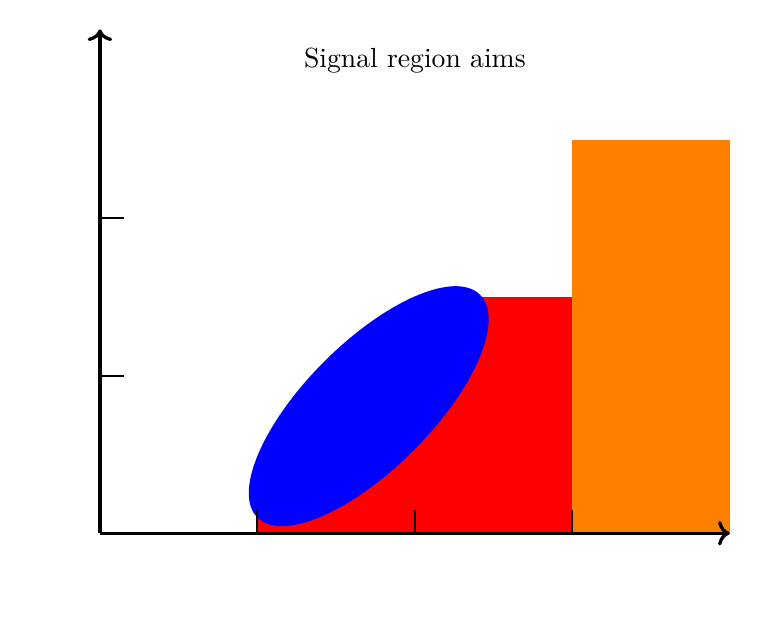
\begin{tikzpicture}[scale = 2]
          \draw[->,thick, line width=1.2] (0, 0) -- (0,3.2);
          \node[black] at (-0.4,2.7) {\mLSP};
          \draw[line width=0.8] (0, 1) -- (0.15,1);
          \draw[line width=0.8] (0, 2) -- (0.15,2);
          %\node[black] at (-0.2,1) {\tiny 100};
          %\node[black] at (-0.2,2) {\tiny 200};
          \fill [orange] (3,0) rectangle (4,2.5);
          \fill [red] (2,0) rectangle (3,1.5);
          \fill [red] (1,0) rectangle (2,0.3);
          \fill [red] (1.5,0) rectangle (2,0.7);

          \fill [blue,rotate around={-135:(1,0.1)}] (1,0.1) arc(0:360:1 and 0.4);

          \draw[line width=0.8] (1, 0) -- (1,0.15);
          \draw[line width=0.8] (2, 0) -- (2,0.15);
          \draw[line width=0.8] (3, 0) -- (3,0.15);
          %\node[black] at (1,-0.1) {\tiny 200};
          %\node[black] at (2,-0.1) {\tiny 400};
          %\node[black] at (3,-0.1) {\tiny 600};
          \node[black] at (3.7,-0.4) {\mstop};
          \draw[->,thick, line width=1.2] (0, 0) -- (4,0);
          \node[black] at (2,3) {Signal region aims};	
        \end{tikzpicture}
\caption[Illustration of signal regions.]{Multiple signal regions have been developed to increase sensitivity in different stop and neutralino mass combinations: SRC in blue, SRB in red, and SRA in orange.} \label{fig:signalregions}
\end{figure}


More details on the SRs are presented in Section \ref{sec:srDefs}.  Signal regions A (SRA) and B (SRB) are optimized for high stop masses.  SRA is optimized to be sensitive to decays of heavy stops into a top quark and a light \LSP. Events are divided into three categories based on the reconstructed top candidate mass, which was not done in the Run 1 analysis. The TT category includes events with two well-reconstructed top candidates, the TW category contains events with a well-reconstructed leading \pt\ top candidate and a well-reconstructed subleading $W$ candidate (from the subleading $R=1.2$ reclustered mass), and the T0 category represents events with only a leading top candidate. This is shown in Figure \ref{fig:categories}. Optimizing the significance\footnote{Significance is defined as $\frac{S}{\sqrt{B}}$ where $S$ is the number of signal events and $B$ is the number of background events} in the categories showed an improvement in discovery significance compared to the combined optimization. \\


\begin{figure}[t]
  \begin{center}
    \includegraphics[width=0.7\textwidth]{figures/SRA/CategoryDefs}
    \caption[Top quark mass categories.]{Illustration of signal-region categories (TT, TW, and T0) based on the $R=1.2$ reclustered top-candidate masses for simulated direct top-squark pair production with $(m_{\stop},m_{\ninoone})=(1000,1) \GeV$ after the loose preselection requirement described in the text. The black lines represent the requirements on the reclustered jet masses.}
    \label{fig:categories}
  \end{center}
\end{figure}

In SRC the signature of stop decays when $\Delta m(\stop,\LSP)\sim m_{t}$ is significantly softer with low \met. This decay topology is very similar to non-resonant \ttbar\ production making signal and background separation challenging. However, several kinematic properties can be exploited to separate stop decays from \ttbar\ when an ISR jet is present in the final state. \\

The selections for SRD are optimized for the decay of both pair-produced top squarks into a $b$ quark and a \chinoonepm. SRE is designed for a model for which the tops are highly boosted. Such signatures can either come from direct stop pair production with a very high stop mass, or in the gluino-mediated compressed-stop scenario with large \mgluino - \mstop. \\

%The analysis is also sensitive to gluino mediated stop production in the case where $\Delta(\mgluino, \mstop)$ is large but $\Delta(\mstop,\mLSP)$ is small. This results in a decay signature that is similar to direct stop production with highly boosted tops and high \met. \\

Background processes that contaminate SRs must also be estimated.  Control regions (CRs) are designed for each dominant background to be pure in that background and have as little signal contamination as possible.  Section \ref{sec:signalContamination} shows the signal contamination in each of the CRs and VRs.  These are compared to data and therefore must be orthogonal to the SRs, but still as close as possible kinematically in order to reduce uncertainties when extrapolating.  The CRs are defined for the major backgrounds in each SR to normalize the simulation to data and ensure the shapes of the simulated backgrounds match those of the data.  However, enough data is required in order to minimize the uncertainties in the normalization factors. \\

The dominant background sources are:

\begin{itemize}
\item $Z\rightarrow \nu \nbar$ plus additional $b$-jets, typically produced in a Drell-Yan process.  
\item Semileptonic $\ttbar$ events, which contain $\Wboson \to e/\mu/\tau \nu$ decays where the lepton is either lost or mis-identified as a jet (and have high \met\ due to the escaping neutrino).
\item $W\rightarrow \ell \nbar$ plus additional $b$-jets, 
\item $\ttbar+\Zboson$, where both tops decay hadronically and $\Zboson\rightarrow \nu \nbar$, and
\item $Wt$-channel single top decays, where one $W$ decays hadronically and one leptonically.
\end{itemize}

Figure \ref{fig:atlasbsmsummaryfiducialxsect} summarizes theory predictions and ATLAS measurements for various SM production cross-sections and shows both total and fiducial cross sections\footnote{A fiducial cross section is a cross section for the subset of a process which is visible in the detector.}.  \\




\begin{figure}[tbh!]
	\centering
	\includegraphics[width=0.9\linewidth]{figures/ATLAS_b_SMSummary_FiducialXsect}
	\caption[SM fiducial production cross sections.]{Summary of several SM total and fiducial production cross section measurements compared to the corresponding theoretical expectations\cite{atlassmsummaryplots}.}
	\label{fig:atlasbsmsummaryfiducialxsect}
\end{figure}

It can be seen in Figure \ref{fig:bkgSRB}, which shows the backgrounds in SRB, that $Z\rightarrow \nu \nbar$ and $\ttbar$ are major contributors to the background processes. \\


\begin{figure}[H] 
\begin{center}
 \includegraphics[width=0.2\textwidth]{figures/barCharts/bkgBarsSRB1.pdf} %\hspace{0.05\textwidth}
 \includegraphics[width=0.2\textwidth]{figures/barCharts/bkgBarsSRB2.pdf} %\hspace{0.05\textwidth}
 \includegraphics[width=0.2\textwidth]{figures/barCharts/bkgBarsSRB3.pdf} %\hspace{0.05\textwidth}
    \caption[Backgrounds in SRB.]{Breakdown of the backgrounds in SRB-TT, -TW, and -T0 from left to right.}
    \label{fig:bkgSRB}
\end{center}
\end{figure}

% CRs are designed to be orthogonal to all SRs while as close to the SR kinematically as possible to reduce uncertainties from the extrapolation.  To reduce uncertainties in normalization factors a lot of data is required.  

The strategy for the CRs are:

\begin{itemize}
	\item 1-lepton: Requires exactly one well-identified lepton in order to be orthogonal to the SRs and treat it as a jet.  This CR is used for leptonically-decaying $W$ bosons, as in the $t\bar{t}$, $W+$jets, and single top backgrounds.  The CRs are orthogonal to 1-lepton searches. 
	\item 2-lepton: Requires exactly two well-defined leptons in order to be orthogonal to the SRs.  This is used to model $Z\rightarrow \nu \nbar$ events, so the invariant mass of the leptons must be that of the $Z$ boson.  These leptons are thus treated as invisible particles and their \pt\ added to the \met.
	\item The $\ttbar+Z$ background uses a photon to model the $Z$ \pt.
	\item The QCD multijet background occurs when jets are mis-modeled to produce fake \met.  To estimate this background jet smearing\cite{jetSmearing} is used, where the\pt\ and jet response function of well-measured jets with low \met\ in data are smeared to simulate jet mismodeling.
\end{itemize} 



More details on the CRs are shown in Section \ref{sec:backgroundEstimation}.  The observed numbers of events in the various control regions are included in a binned profile likelihood fit\cite{likelihoodFit} to determine the SM background
estimates for \Zboson, \ttbar, \Wboson, single top, and \ttZ\ in each signal region. 
The normalizations of these backgrounds are determined simultaneously to best match the observed data in each control region taking contributions from all backgrounds into account. A likelihood function is built as the
product of Poisson probability functions, describing the observed and
expected number of events in the control regions\cite{histFitter}. This procedure takes common systematic uncertainties (discussed in
Section \ref{sec:Systematics}) between the control and signal regions and
their correlations into account as they are treated as nuisance
parameters in the fit and are modeled by Gaussian probability density
functions. %The free parameters in the fit are the overall normalisations of the backgrounds listed in Table~\ref{table.scale.factors}. %needs more description of combinations, etc
The contributions from all other background processes (dibosons and multijets) are fixed at the values expected from
the simulation, using the most accurate theoretical cross sections
available, while their uncertainties are used as nuisance parameters in the fit. \\


%%The CRs are fit to data in order to normalize the background estimates the simulation.  

%%Transfer factors
%The background estimates are scaled using normalization factors computed from the fit.  The normalization factors are used as:
%
%\begin{equation}
%N_{p}(\rm{SR,est.}) = N_{p}(\rm{CR,obs.}) \times [\frac{MC_{p}(\rm{SR,raw.}) }{MC_{p}(\rm{CR,raw.}) }]= \mu_{p} \times MC_{p}(\rm{SR,raw.})  
%\end{equation}
%
%where $N_p$ is the SR background estimate for each simulated process $p$, obs. refers to the number of data events and raw refers to the estimates from MC simulation, and $\mu_p$ is the normalization factor.  The ratio in brackets is defined as the transfer factor (TF).  A feature of the TFs is that systematic uncertainties on background processes can be canceled in the extrapolation.  \\

Validation Regions (VRs) are designed to validate the factors determined in the CRs and are a region orthogonal to both the SR and the CR while between the two kinematically, e.g. 0-lepton validation regions are closer kinematically than a 1- or 2-lepton CR.  \\

The validation regions for \Zboson +jets avoids overlap with the signal region by reversing the \drbjetbjet\ and/or the \mantikttwelvezero/\mantikteightzero\ requirement.  The validation regions for $t\bar{t}$ avoids overlap with the signal regions by reversing the \mtbmin requirement.  More details on the VRs are shown in Section \ref{sec:backgroundEstimation}.  \\



There are also important checks on the data and simulation that must be performed in order to be confident in the results.  For this analysis the following checks were performed:

\begin{itemize}
	\item Checking the dependence of discriminating variables on pileup to ensure that different pileup conditions do not affect the analysis.  
	\item Checking for problems with specific runs by making sure that the data yields normalized by luminosity are consistent.
	\item Checking for any missing data by comparing processed data to reference numbers.  
	\item Checking for duplicate events in simulation as previous productions contained a bug that caused this.  This can cause regions to be mis-modeled.
	\item Checking the debug stream for any events in CRs and SRs.  The debug stream catches events in which the trigger was unable to make a decision due to some failure in the online system.
	\item Checking the pileup reweighting to make sure that the pileup weight for simulation matches data after applying the weight.
\end{itemize}

The checks helped to validate the data and simulation and the data is stable and have high quality.  Figure \ref{fig:nvtxSanityChecks} show the dependence on pileup for \mantikttwelvezero\ and \met. The full results for several of these checks are shown in Appendix \ref{sec:Standard_Checks}. \\

\begin{figure}[tbh]
	\centering
		\includegraphics[width=0.32\textwidth]{figures/sanityChecks/RC12MassLeadingNvtxProfileMCData.eps}	
		\includegraphics[width=0.32\textwidth]{figures/sanityChecks/MetNvtxProfileMCData.eps}
		\includegraphics[width=0.32\textwidth]{figures/sanityChecks/NJetsNvtxProfileMCData.eps}
	\caption[Checks on the dependence of pileup of \mantikttwelvezero, \met, and jet multiplicity.]{\label{fig:nvtxSanityChecks}{Checks on the dependence of pileup of \mantikttwelvezero, \met, and jet multiplicity.  Ideally there is no dependence and the distributions are flat.}}
\end{figure}


After the normalization factors have been validated, the background predictions are extrapolated to the SRs and then the data is ``unblinded," and the SRs are compared to observed data.  For discovery a p-value is calculated in each SR and subregion independently.  \\

%Probability density functions (PDFs) are used to extract information from data.  The parameters of the PDF are adjusted with the fitting procedure and the fit is based on independent CRs and SRs, but parameters can be shared across all CRs, VRs, and SRs.  This PDF describes the parameters of interest like the signal process rate and normalization factors, and the nuisance parameters that parameterize the impact of systematic uncertainties.  These parameters 

%The general likelihood of the analyses is the product of Poisson distributions of event counts in the SRs and CRs along with distributions implementing constraints on systematic uncertainties.  
%
%There are three commonly-used types of fits that can be performed:
%
%\begin{itemize}
%	\item Background-only fit: the purpose of this fit is to estimate total background in SRs and VRs without any assumption of a signal model, so using only background samples.  This is only performed in the CRs and the fits are normalized to the observed event counts.  This can also be useful for other groups to perform a hypothesis test on a different signal model.  
%	\item Model-dependent signal fit: this is used for a specific signal model.  When there is no significant event excess in the SRs, determined by the background-only fit, exclusion limits can be set, or in the case of an excess the signal strength can be measured.  This is performed in the CRs and SRs simultaneously and include a signal sample in all regions to account for signal contamination in the CRs with a normalization factor assigned to the signal sample.  If SRs and CRs are statistically independent and non-overlapping this can be performed simultaneously in multiple CRs and SRs.  Multiple SRs sensitive to the same signal model can also be statistically combined to give better exclusion sensitivity.  
%		\begin{itemize}
%		\item In this analysis a grid of signal samples with varying masses of \stop\ and \ninoone\ and this fit is repeated for each of these grid points in order to probe the phase space of the model.
%		\end{itemize}
%	\item Model-independent signal fit: this is used for setting upper limits independent of a model on the number of events in each SR analyses searching for new physics phenomena.  This way, for any signal model of interest, the number of signal events predicted in a SR can be estimated and it can be seen if that model is already excluded.  
%\end{itemize}


For the exclusion fits, the subregions of SRA, SRB, and SRC are statistically combined.  Then SRA, B, C, D, and E are combined by taking the result with the best expected CL\textsubscript{s}\cite{CLs1, CLs2}.  As no excess is observed in any of the signal regions, new limits are placed on SUSY masses in the \mstop}-$m_{\ninone}$, as shown in Figure  as well as in terms of $m_{\gluino}-\mstop$.  Additionally, results are interpreted in terms of the pMSSM and several models have new exclusion limits.  There are more details on the exclusions in Section \ref{sec:results}.  \\

\begin{figure}[htpb]
  \begin{center} \includegraphics[width=0.7\textwidth]{figures/atlascls_m0m12_wband1_showcms0_StopZL2016_SRABCDE_Tt_directTTplusbWN_all_Output_fixSigXSecNominal_hypotest__1_harvest_list.pdf}%
    \caption[Exclusion contours in as a function of $\stop$ and $\ninoone$ masses in the scenario where both top squarks decay via $\stop\to t^{(*)} \ninoone$]{Observed (red solid line) and expected (blue solid line)
      exlusion contours at 95\% CL as a function of $\stop$ and
      $\ninoone$ masses in the scenario where both top squarks decay
      via $\stop\to t^{(*)} \ninoone$. Masses that are lower than the masses along the lines are excluded. Uncertainty bands corresponding to the $\pm 1
      \sigma$ variation on the expected limit (yellow band) and the
      sensitivity of the observed limit to $\pm 1\sigma$ variations of
      the signal theoretical uncertainties (red dotted lines) are also
      indicated. Observed limits from all third-generation Run-1 searches~\cite{Atlas8TeVSummary} at $\sqrt{s}=8$ TeV centre-of-mass energy are overlaid for comparison in blue.}
    \label{fig:SRABC_exclusion}%\label{fig:SRD4_exclusion}
  \end{center}
\end{figure}

%In order to maximize sensitivity for SRA and SRB, final state categories based on top reconstruction were developed.  There are three cases: two top candidates are successfully reconstructed, a top and a $W$ boson are reconstructed, and one top is reconstructed but no second top or $W$ are reconstructed.  Cuts were decided for each category to maximize sensitivity in each.  








\chapter{Event Reconstruction}

\section{Particle Identification}
\subsection{Tracks}
\subsection{Topoclusers}

\section{Jets}
%reconstruction, topoclustering, digitization path, etc
\section{Electrons}
\section{Photons}
\section{Muons}
\section{Taus}
\section{Missing Transverse Momentum}
\section{Monte Carlo Simulations}
\chapter{Analysis}
\label{ch:analysis}



This chapter describes the analysis in depth, beginning with the signal regions and continuing with background estimation and finally presenting the results, interpretations, and outlook.  The lightest supersymmetric partner to the top quark\footnote{There is a SUSY partner to the helicity states of the top quark in the SM, $\tilde{t}_{L}$ and $\tilde{t}_{R}$, which mix to form the $\tilde{t}_{1}$ and $\tilde{t}_{2}$ where the $\tilde{t}_{1}$ is the lightest of the two.} being produced in direct pair production is the main focus of the analysis, while other scenarios are also discussed.  

%\section{Object Selection}

%The object definitions used follow the ATLAS recommendations and SUSY group standards.


\section{Signal Region Definitions}
\label{sec:srDefs}

Leading order stop pair-production at the LHC is expected to be dominated by gluon fusion, then by the subprocess $q\bar{q}$ annihilation.  The stops are pair produced, conserving $R-$parity, and are produced directly, so there are no intermediate particles in the simplified model.  \\

As discussed in Chapter \ref{ch:analysisOverview} there are five distinct signal regions developed to optimize discovery significance for different topologies, SRA-E.  All of the searches share the following preselection requirements:

\begin{itemize}
	\item For data samples, events must be in the Good Runs List (GRL), which are runs that pass certain data quality requirements.%  This gives a total luminosity of 36.1 fb\textsuperscript{-1}.
	\item For data samples, Must pass cleaning selection which removes events with incomplete data or with calorimeter noise bursts.
	\item The event must pass the lowest unprescaled \met\ trigger as well as have offline \met\ $>$ 250 GeV.
	\item The event must have a reconstructed primary vertex.
	\item The event must not contain any ``bad jets" from the jet definition described in section \ref{section:jetcleaning} with \pt\ $>$ 20 GeV. %``BadLooser"
	\item The event must not contain any cosmic muons as discussed in section \ref{section:jetcleaning}
	\item The event must not contain any bad muons as described in section \ref{section:muons}.
	\item The event must contain no baseline electron candidates with \pt\ $>$ 7 GeV and no baseline muons with \pt\ $>$ 6 GeV.
	\item The event must contain at least four jets.
	\item The \dphi\ between the leading two (three) jets and the \met, \dphijettwomet, (\dphijetthreemet), must be greater than 0.4 for ISR based regions (non-ISR based regions). 
	\item The \mettrk\ must be greater than 30 GeV.
	\item The \dphi, between the calo \met\ and the \mettrk, \dphimettrk, must be smaller than $\pi/3$.
\item At least one b-tagged jet at the 77\% working point is required.
\end{itemize}

The analysis relies heavily on reconstruction top quark candidates, which is done using jet ``reclustering."  Jet reclustering is performed using the \antikt\ algorithm with a larger distance parameter (i.e. $R=1.2$) over the calibrated \antikt\ $R=0.4$ jet collection. The highest (second-highest) \pT\ reclustered jet is designated as the first (second) top candidate. Various optimization studies have found that this method using $R=1.2$ (top candidate) and $R=0.8$ ($W$ candidate) results in the best signal sensitivity. The mass distribution is shown in Figure \ref{fig:preselection}.  The masses are indicated by \mantikttwelvezero, \mantikttwelveone, \mantikteightzero, \mantikteightone. \\



A suite of discriminating variables based on \antikt\ $R=0.4$ jets will be considered in the analysis optimization: 
\begin{itemize}
	\item $\dphijettwomet$: The difference in $\phi$ between the jet and \met\ for the two leading jets in the event. This variable rejects events with fake \met\ from QCD, hadronic \ttbar, and detector effects.
	\item $\HT$: The scalar sum of the \pt\ of all signal \antikt\ $R=0.4$ jets ($\pt>20\gev$, $|\eta|<2.8$, after overlap removal).
	\item $\mtjetimet$: The transverse mass (\mt) between the $i$th jet and the \met\ in the event. The massless approximation is used for this and all following \mt\ variables:\newline $\mtjetimet = \sqrt{2\ptjeti\met\left(1-\cos{\Delta\phi\left(\mathrm{jet}^i,\met\right)}\right)}$, where $\ptjeti$ is the transverse momentum of the $i$th jet.
	\item $\mtbmin$: Transverse mass between closest $b$-jet to $\met$ and $\met$. This variable provides the most powerful discrimination between signal and semileptonic \ttbar\ background.
	\item $\mtbmax$: Transverse mass between furthest $b$-jet to $\met$ and $\met$. This variable provides very good discrimination between signal and semileptonic \ttbar\ background.
	\item $\drbb$: The angular separation between the two jets with the highest $b$ weights. This variable is useful in discriminating against the $Z(\nu\overline\nu)+b\overline{b}+\rm{jets}$ background. %MV2c10
\end{itemize}

A common preselection used for all five sets of signal regions is defined in Table~\ref{tab:SRcommon}.  % while the details of each signal region is given in section~\ref{sec:SignalRegionAB},~\ref{sec:SignalRegionC},~\ref{sec:SignalRegionD},~\ref{sec:SignalRegionE}.

Distributions of (a)~\mantikttwelvezero\ and (b)~\mtbmin\ are shown in Figure \ref{fig:preselection}.  

\begin{figure}[t]
  \begin{center}
    \subfloat[]{\includegraphics[width=0.5\textwidth]{figures/preselection/AntiKt12M0_preCutSRPlot_withRatio}}
    \subfloat[]{\includegraphics[width=0.5\textwidth]{figures/preselection/MtBMin_preCutSRPlot_withRatio}}
    \caption[Distributions of the discriminating variables \mantikttwelvezero\ and \mtbmin\ after common preselection.]{Distributions of the discriminating variables (a)~\mantikttwelvezero\ and (b)~\mtbmin\ after the common preselection and an additional $\mtbmin>50\gev$ requirement. The stacked histograms show the SM prediction before being normalized using scale factors derived from the simultaneous fit to all dominant backgrounds. The ``Data/SM" plots show the ratio of data events to the total SM prediction. The hatched uncertainty band around the SM prediction and in the ratio plots illustrates the combination of statistical and detector-related systematic uncertainties. The rightmost bin includes overflow events.}
    \label{fig:preselection}
  \end{center}
\end{figure}
\clearpage


\begin{table}[htbp]
  \caption[Signal region selection criteria.]{Selection criteria common to all signal regions.  Different triggers were used for different data periods in 2016.}
  \begin{center}
    \begin{tabular}{l|c} \hline\hline
      Trigger & Data 2015: \verb+HLT_xe70_mht_L1XE50+ \\ %\hline
              & Data 2016: \verb+HLT_xe90_mht_L1XE50+, \\  
              &  \verb+HLT_xe100_mht_L1XE50+,  \\ 
              &  \verb+HLT_xe110_mht_L1XE50+  \\ %\hline
              & \\ [-2.5ex] \hline
      $\met$ & $> 250\GeV$ \\ %\hline
              & \\ [-2.5ex] \hline
      $N_{\rm{lep}}$ & 0 \\ \hline
      \antikt\ $R=0.4$ jets & $\ge 4,~\pt>80,80,40,40 \gev$ \\ \hline
      $b$-tagged jets & $\ge1$ \\ \hline
      % $\dphijettwomet$ & $> \pi/5$ \\ 
      $\dphijettwomet$ or $\dphijetthreemet$ & $> 0.4$ \\ 
              & \\ [-2.5ex] \hline
      $\mettrk$  & $> 30 \gev$ \\ \hline 
      % & \\ [-2.5ex]
      $\dphimettrk$ & $<\pi/3$ \\ \hline
      % & \\ [-2.5ex] \hline
      % $\tau$ veto & yes \\ \hline
      % $\mtbmetmindphi$ & $> 175 \gev$ \\ \hline \hline
    \end{tabular}
  \end{center}
  \label{tab:SRcommon}
\end{table}

\subsection{SRA and SRB}

SRA and SRB are optimized for high stop masses.  In addition to the preselection, SRA and SRB have common requirements of $\mtbmin>200\gev$, which reduces $t\bar{t}$ background,  two b-tagged jets, and a $\tau$-veto. \\

SRA is optimized to be sensitive to decays of heavy stops into a top quark and a light \LSP. The main discriminating variables are the reclustered top masses, with $R=1.2$ and $R=0.8$, \mtbmin, \drbjetbjet, and \met. Events are divided into three categories based on the reconstructed top candidate mass ($R=1.2$ reclustered jet mass). The TT category includes events with two well-reconstructed top candidates, the TW category contains events with a well-reconstructed leading \pt\ top candidate and a well-reconstructed subleading $W$ candidate (from the subleading $R=1.2$ reclustered mass), and the T0 category represents events with only a leading top candidate. \\

The categorization showed an improvement in discovery significance, assuming the shape of the $\mstop=800\gev,\mLSP=1\gev$ benchmark, from 2$\sigma$ to 3$\sigma$, yielding comparable results to a boosted decision tree (BDT). For the benchmark point with $\mstop=1000\gev,\mLSP=1\gev$, after the SRA-B preselection, $\sim$91\% (TT=38\%, TW=22\%, and T0=31\%) of events fall into one of these three categories.  \\ %In addition to the requirements listed in Table~\ref{tab:SRcommon}, SRA and SRB have common requirements of $\mtbmin>200\gev$, two b-tagged jets, and a $\tau$-veto (in addition to the preselection cuts).   \\ %NOTE: include BDT studies?

Additionally, requirements on the stransverse mass (\mttwo)~\cite{Lester:1999tx,Barr:2003rg}
are made which are especially powerful in the T0 category where a $\chi^2$ method is applied to reconstruct top quarks with lower momenta where reclustering was suboptimal. 
The \mttwo\ variable is constructed from the direction and magnitude of the \ptmiss\ vector in the transverse plane as well as the direction of two top-quark candidates reconstructed using a $\chi^2$ method. 
The minimization in this method is done in terms of a $\chi^2$-like penalty function, $\chi^2 = (m_{\mathrm{cand}}-m_{\mathrm{true}})^2/m_{\mathrm{true}}$, where $m_{\mathrm{cand}}$ is the candidate mass and $m_{\mathrm{true}}$ is set to 80.4 GeV for \Wboson\ candidates and 173.2 GeV for top candidates. 
Initially, single or pairs of $R=0.4$ jets form \Wboson\ candidates which are then combined with additional $b$-tagged jets in the event to construct top candidates. The top candidates selected by the $\chi^2$ method are only used for the momenta in \mttwo\ while the mass hypotheses for the top quarks and the invisible particles are set to 173.2 GeV and 0 GeV, respectively. \\

A similar strategy was taken for the optimization of SRB which is aimed at being sensitive to $\mstop=600\gev,\mLSP=300\gev$. In addition to the \met\ and reclustered masses, \mtbmax, \mtbmin, and \drbjetbjet\ were used in the optimization.  The fraction of events in each category is after the SRA-B preselection: TT=14\%, TW=20\%, T0=35\%. All three categories are used in the optimization resulting in the signal regions defined in Table~\ref{tab:SignalRegionAB}. \\

\begin{table}[htb]
  \caption[Selection criteria for SRA and SRB.]{Selection criteria for SRA and SRB, in addition to the common preselection requirements as shown in Table \ref{tab:SRcommon}. The signal regions are separated into topological categories based on reconstructed top-candidate masses.}
  \begin{center}
  \def\arraystretch{1.4}
   \begin{tabular}{c||l|c|c|c} \hline\hline
      {\bf Signal Region}      &                    & {\bf TT}    & {\bf TW}     & {\bf T0}     \\ \hline \hline
                               & \mantikttwelvezero & \multicolumn{3}{c}{$>120\gev$}            \\ \cline{2-5}
                               & \mantikttwelveone  & $>120\gev$  & $[60,120]\gev$ & $<60\gev$    \\ \cline{2-5}
                               & \mtbmin            & \multicolumn{3}{c}{$>200\gev$}            \\ \cline{2-5}
                               & \nBJet    & \multicolumn{3}{c}{$\ge2$}                \\ \cline{2-5}
                               & $\tau$-veto        & \multicolumn{3}{c}{yes}                   \\ \cline{2-5} 
                               & \dphijetthreemet   & \multicolumn{3}{c}{$>0.4$}                \\ \cline{2-5}\hline \hline
      \multirow{3}{*}{{\bf A}} & \mantikteightzero  & \multicolumn{3}{c}{$>60\gev$}             \\ \cline{2-5}
                               & \drbjetbjet        & $>1$        & \multicolumn{2}{c}{-}       \\ \cline{2-5}
                               & \mttwo             & $>400$ GeV  & $>400$ GeV   & $>500$ GeV   \\ \cline{2-5}
                               & \met               & $>400 \gev$ & $> 500 \gev$ & $> 550 \gev$ \\ \hline \hline
      \multirow{2}{*}{{\bf B}} & \mtbmax            & \multicolumn{3}{c}{$>200\gev$}            \\ \cline{2-5}
                               & \drbjetbjet        & \multicolumn{3}{c}{$>1.2$}                \\ \cline{2-5}              
\hline\hline
    \end{tabular}
\end{center}
\label{tab:SignalRegionAB}
\end{table}


%Distributions of discriminating variables for SRA and SRB are shown in Figures \ref{fig:SRAMetAntiKt8M} and \ref{fig:SRBDRBBMtBMax} respectively, including the benchmark points.  Note that cutting on the variables reduces background more than it reduces the signal, thus improving sensitivity.  \\
%
%\begin{figure}[htb]
%	\begin{center}
%		\includegraphics[width=0.445\textwidth]{figures/Met_SRA_TT.eps} 
%		\includegraphics[width=0.445\textwidth]{figures/AntiKt8M_0__SRA_TT.eps} \\
%		\includegraphics[width=0.445\textwidth]{figures/Met_SRA_TW.eps} 
%		\includegraphics[width=0.445\textwidth]{figures/AntiKt8M_0__SRA_TW.eps} \\
%		\includegraphics[width=0.445\textwidth]{figures/Met_SRA_T0.eps} 
%		\includegraphics[width=0.445\textwidth]{figures/AntiKt8M_0__SRA_T0.eps}
%		\caption[Distributions of the \met\ and the \mantikteightzero\ for SRA]{\label{fig:SRAMetAntiKt8M} Distributions of the \met\ and the \mantikteightzero\ for SRA-TT, SRA-TW, and SRA-T0 after all requirements (except for the \met\ and \mantikteightzero, respectively) of Table~\ref{tab:SignalRegionAB} are made. The stacked histogram represent the total expected background estimated from MC while the hashed area represents the uncertainty due to MC statistics. Signal is shown in dashed and dotted lines for the $\mstop=600\gev,\mLSP=300\gev$ and $\mstop=1000\gev,\mLSP=1\gev$ benchmarks, respectively. }
%	\end{center}
%\end{figure}
%\clearpage
%
%\begin{figure}[!htb]
%	\begin{center}
%		\includegraphics[width=0.445\textwidth]{figures/DRBB_SRB_TT.eps}
%		\includegraphics[width=0.445\textwidth]{figures/MtBMax_SRB_TT.eps}\\
%		\includegraphics[width=0.445\textwidth]{figures/DRBB_SRB_TW.eps}
%		\includegraphics[width=0.445\textwidth]{figures/MtBMax_SRB_TW.eps}\\
%		\includegraphics[width=0.445\textwidth]{figures/DRBB_SRB_T0.eps}
%		\includegraphics[width=0.445\textwidth]{figures/MtBMax_SRB_T0.eps}\\
%		\caption[Distributions of the \drbb\ and the \mtbmax\ for SRB]{\label{fig:SRBDRBBMtBMax} Distributions of the \drbb\ for SRB-TT, SRB-TW, SRB-T0 and after all requirements except for the \drbb\ of Table~\ref{tab:SignalRegionAB} are made. The \mtbmax\ distributions are also shown with all but the \mtbmax\ requirements made.  The stacked histogram represent the total expected background estimated from MC while the hashed area represents the uncertainty due to MC statistics. Signal is shown in dashed and dotted lines for the $\mstop=600~\gev,\mLSP=300~\gev$ and $\mstop=1000~\gev,\mLSP=1~\gev$ benchmarks, respectively. }
%	\end{center}
%\end{figure}
%\clearpage


 
%To interpret the results the p-values are reported in each category along with the combined p-value.  

%SRC
\subsection{SRC}
\label{sec:SRC}
The signature of stop decays when $\Delta m(\stop,\LSP)\sim m_{t}$ is significantly softer with low \met. This decay topology is very similar to non-resonant \ttbar\ production making signal and background separation challenging. However, several kinematic properties can be exploited to separate stop decays from \ttbar\ when an ISR jet is present in the final state. \\

An additional set of discriminating variables is defined for signal regions using ISR to gain sensitivity the compressed ($\mstop-\mLSP\sim m_t$) signal grid region. These variables are all defined in the transverse center-of-mass (CM) of the sparticle plus ISR frame. Visible objects are grouped into being either a part of the ISR or the sparticle system. This is performed using a recursive jigsaw reconstruction technique\cite{RJR_ISR}, which looks for a ``thrust axis" where the \pt-projection of all jets and \met\ in the center of mass frame in the event are maximized.  This axis then divides the space into the sparticle or ISR system.  This association with the ISR or sparticle system is indicated by an ISR or S superscript, respectively. The ``V" subscript denotes the visible part of system.  For example, \mV\ denotes the transverse mass of only the visible (jets+leptons) part of the sparticle system without the \met.  The variables considered are:

\begin{itemize}
\item  \nBJetS: number of b-tagged jets associated with the sparticle hemisphere.
\item \nJetS: number of jets associated with the sparticle hemisphere.
\item  \pTSBZero: \pt\ of the leading b-jet in the sparticle hemisphere.
\item  \pTSFour: \pt\ of the fourth jet ordered in \pt\ in the sparticle hemisphere.
\item  \dPhiISRMET: angular separation in $\phi$ of the ISR and the \met in the CM frame.
\item  \pTISR: \pt\ of the ISR system, evaluated in the CM frame.
\item  \mS: transverse mass between the whole sparticle system and \met.
\item  \mV/\mS: ratio of the transverse mass of the only the visible part of the sparticle system without \met and the whole sparticle system including \met.
\item  \rISR: Ratio between invisible system (\met in CM frame) and \pTISR
\end{itemize}

After the preselection, defined in Table~\ref{tab:SRcommon},
additional requirements are made resulting in five signal regions,
SRC-1 through SRC-5, for which the exact requirements are listed in
Table~\ref{tab:SignalRegionC}. 

\begin{table}[htpb]
  \caption[Selection criteria for SRC]{Selection criteria for SRC, in addition to the common preselection requirements as shown in Table \ref{tab:SRcommon}. The signal regions are separated into windows based on ranges of $\RISR$.}
  \begin{center}
    \def\arraystretch{1.4}
    \begin{tabular}{c||c|c|c|c|c} \hline\hline
      {\bf Variable} & SRC1 & SRC2 & SRC3 & SRC4 & SRC5 \\ \hline \hline
       \nBJet & \multicolumn{5}{c}{$\ge1$} \\ \hline
      \nBJetS & \multicolumn{5}{c}{$\ge1$} \\ \hline
      \nJetS & \multicolumn{5}{c}{$\ge5$}  \\ \hline
      \pTSBZero & \multicolumn{5}{c}{$>40\gev$}  \\ \hline
      \mS & \multicolumn{5}{c}{$>300\gev$}  \\ \hline
      \dPhiISRMET & \multicolumn{5}{c}{$>3.0$}  \\ \hline
      \pTISR & \multicolumn{5}{c}{$>400$ GeV}   \\ \hline
      \pTSFour & \multicolumn{5}{c}{$>50$ GeV}   \\ \hline
      \rISR & 0.30--0.40 & 0.40--0.50 & 0.50--0.60 & 0.60--0.70 & 0.70--0.80\\  \hline \hline
    \end{tabular}
  \end{center}
  \label{tab:SignalRegionC}
\end{table}





%SRD

\subsection{SRD}

The selections for SRD are optimized for the decay of both pair-produced top squarks into a $b$ quark and a \chinoonepm. In this case no top-quark candidates are reconstructed, so the sum of the transverse momenta of the two jets with the highest $b-$tagging weight, as well as that of the second, fourth, and fifth highest, are used for additional background rejection.  The models considered for the optimization have the chargino mass fixed to two times the neutralino mass, $m(\chinoonepm) = 2 \cdot m(\ninoone)$. \\

The best selections for the signal samples with m(\stop) = 400 GeV, m(\ninoone) = 50 GeV (SRD-low), %m(\stop) = 600 GeV, m(\ninoone) = 100 GeV (SRD-med), 
m(\stop) = 700 GeV, m(\ninoone) = 100 GeV (SRD-high) are reported in Table~\ref{tab:SRDsel}. The two regions are not combined, individual p-values are quoted for discovery while the region with the best expected sensitivity is chosen during the exclusion fit.

\begin{table}[!htb]
  \caption[Selection criteria for SRD]{Selection criteria for SRD, in addition to the common preselection requirements as shown in Table \ref{tab:SRcommon}.}
  \begin{center}
  \def\arraystretch{1.4}
  \begin{tabular}{c||c|c}
    \hline\hline
    {\bf Variable}       & {\bf SRD-low} & {\bf SRD-high} \\
    \hline \hline
    \dphijetthreemet     & \multicolumn{2}{c}{$>0.4$}     \\ \hline
    \nBJet      & \multicolumn{2}{c}{$\geq$2}    \\\hline
    \drbjetbjet     & \multicolumn{2}{c}{$>$ 0.8}    \\ \hline
    \ptbzero+\ptbone & $>300$ GeV    & $>400$ GeV     \\ \hline
    $\tau$-veto          & \multicolumn{2}{c}{yes}        \\ \hline
    \ptone\              & \multicolumn{2}{c}{$>150\GeV$} \\ \hline
    \ptthree\            & $>100\GeV$    & $>80\GeV$      \\ \hline
    \ptfour\             & \multicolumn{2}{c}{$>60\GeV$}  \\ \hline
    \mtbmin\             & $>250\GeV$    & $>350\GeV$     \\ \hline
    \mtbmax\             & $>300\GeV$    & $>450\GeV$     \\ 
    \hline\hline
  \end{tabular}
  \end{center}
  \label{tab:SRDsel}
\end{table}


\subsection{SRE}

SRE is designed for a model for which the tops are highly boosted. Such signatures can either come from direct stop pair production with a very high stop mass, or in the gluino-mediated compressed-stop scenario with large $\mgluino - \mstop$. The benchmark for this signal region is a model where $(\mgluino, \mstop, \mLSP) = (1700, 400, 395) \gev$. Due to the large boost, the top daughters are more collimated compared to typical topology expected in \SRA.  Compared to direct stop pair production with $\mstop=800 \gev$ and $\mLSP=1 \gev$, the $\Delta R$ separation between the \Wboson\ and the bottom quark tends to be smaller. This is shown in Figure \ref{fig:SRBoost_dRWb}.  Therefore, \antikt\ $R=0.8$ reclustered jet collection will be considered as the top candidates instead of $R=1.2$ masses in other signal region. Table~\ref{tab:SignalRegionE} shows the selection criteria for SRE. 

\begin{table}[!htb]
  \caption[Selection criteria for SRE]{Selection criteria for SRE in addition to the common preselection requirements as shown in Table \ref{tab:SRcommon}.}
  \begin{center}
  \def\arraystretch{1.4}
  \begin{tabular}{c||c}
    \hline\hline
    {\bf Variable}    & {\bf SRE}          \\
    \hline \hline
    \dphijetthreemet  & $>0.4$             \\ \hline
    \nBJet   & $\geq$2            \\     \hline
    \mantikteightzero & $>120$ \gev        \\     \hline
    \mantikteightone  & $>80$ \gev         \\     \hline
    \mtbmin\          & $>200$ \gev        \\     \hline
    \met\             & $> 550 \gev$       \\     \hline
    \HT               & $>800 \gev$        \\     \hline
    \htsig            & $> 18 \sqrt{\GeV}$ \\     
\hline\hline
  \end{tabular}
  \end{center}
  \label{tab:SignalRegionE}
\end{table}

\begin{figure}[h]
	\centering
	%\begin{subfigure}[b]{0.45\textwidth}
		%\includegraphics[width=\textwidth]{figures/dRWbT800L1}
		%\caption{$m(\stop,\ninoone)=(800,1)~\GeV$}
		%\label{fig:SRBoost_dRWb_T800L1}
	%\end{subfigure}
	%~ %add desired spacing between images, e. g. ~, \quad, \qquad, \hfill etc. 
	%(or a blank line to force the subfigure onto a new line)
	%\begin{subfigure}[b]{0.45\textwidth}
		%\includegraphics[width=\textwidth]{figures/dRWbGtc5_1400_400}
		%\caption{$m(\gluino,\stop,\ninoone)=(1400,400,395)~\GeV$}
		%\label{fig:SRBoost_dRWb_Gtc_1400_400}
	%\end{subfigure}
	\includegraphics[width=\textwidth]{figures/drTruthSRE.pdf}
	\caption[$\Delta R$ between the \Wboson\ and the $b$-quark vs. the top \pt]{The true $\Delta R$ between the \Wboson\ and the $b$-quark vs.\ the truth top \pt\ for (a) SRA and (b) SRE. The common preselection criteria are applied with the exception of the $b$-jet requirement.}
	\label{fig:SRBoost_dRWb}
\end{figure}

\section{Background Estimation}
\label{sec:backgroundEstimation}


%SRAB





% followed by $t\bar{t}$.  In  \ttbar+V. The next three dominant backgrounds for each of the categories have about equal contributions and are, \ttbar, and W+jets. Where statistically possible separate control regions are used for the TT, TW, and T0 categories for the dominant backgrounds. \\ %For the Z+jets background normalization a set of two-lepton, two b-tagged jet control regions (described in Sect.~\ref{sec:ZllCR}) are used while for the \ttbar\ and W+jets normalization two orthogonal sets of one-lepton control regions (described in Sect.~\ref{sec:TopCRdef} and Sect.~\ref{sec:WCR}) are used. The \ttbar+V normalization is derived from a one-lepton $\ttbar+\gamma$ control region.



%Z
\subsection{\boldmath$Z+$jets}

The $Z \rightarrow \nu\nu$+jets background becomes more relevant as the \MET\ requirement is tightened. A possible way to estimate the $Z \rightarrow
\nu \nu$ background is by using a $Z \rightarrow \ell \ell$+jets control
sample. The latter channel has the advantage of an easier selection of
pure samples in terms of non-$Z$ background, but it is characterized by a
lower branching fraction than the background that it is trying to
estimate due to the  axial-vector couplings of the charged leptons to the $Z$.  This becomes particularly problematic when estimating the
background for events with large $Z$ \pT\ where the number of expected
events becomes very small. In the current analysis the number of
$Z$+jets events is reduced by the \MET\ selection, the high jet
multiplicity and the requirement for 2 $b-$tagged jets.


   
\subsubsection{Control Region}
%CR
A control region is designed for TT and TW in SRA and SRB and for T0 in SRA and SRB, as well as for SRD and SRE.  A CR for SRC was not developed since there is negligible background from $Z+$jets.  A summary of the CR selections can be found in Table~\ref{tab:selectionCRZs} and the lepton triggers used in the analysis are shown in Table \ref{tb:lepTriggers}.  \\

%INT note:
%\begin{table}[htpb]
%  \caption{Selection for the $Z$ CR with 2 b-jets.}
%  \begin{center}
%    \begin{tabular}{c|c|c|c|c}
%      \hline \hline
%      Selection                 & CRZAB-TT-TW & CRZAB-T0 & CRZD & CRZE       \\
%      \hline \hline
%      Leptons selection & \multicolumn{4}{c}{exactly 2 opposite charge electrons or muons} \\
%      %Leptons \pt & \multicolumn{4}{c}{28 GeV} \\
%      \hline
%      Jet multiplicity & \multicolumn{2}{c|}{$ \ge4 $} & $\ge5$ & $\ge4$ \\
%      \hline      
%      Jet \pT\ & \multicolumn{4}{c}{(80,80,40,40) GeV} \\
%      \hline
%      Lepton invariant mass & \multicolumn{4}{c}{$86 < M(\ell\ell) < 96$ GeV} \\
%      \hline
%      $E_{T}^{miss}$  & \multicolumn{4}{c}{$ < 50$ GeV} \\
%      \hline
%      \metprime &\multicolumn{4}{c}{$ > 100$ GeV} \\
%      \hline
%      b-jets & \multicolumn{4}{c}{$ >=2 $}\\
%      \hline
%      \mantikttwelvezero & \multicolumn{2}{c|}{$>120$ GeV} & \multicolumn{2}{c}{-} \\
%      \hline
%      \mantikttwelveone & $>60$ GeV& $<60$ GeV & \multicolumn{2}{c}{-} \\
%      \hline
%      \mtbminprime &  \multicolumn{2}{c|}{-} & 200 & 200 \\
%      \hline 
%      \mtbmaxprime &  \multicolumn{2}{c|}{-} & 200 & - \\
%      \hline 
%      \HT &  \multicolumn{3}{c|}{-} & 500  \\
%      \hline\hline
%    \end{tabular}
%  \end{center}
%  \label{tb:selectionZllCR}
%\end{table}

\begin{table}[htpb]
  \caption{Selection criteria for the $\Zjets$ control regions used to estimate the $\Zjets$ background contributions in the signal regions.} 
  \begin{center}
    \def\arraystretch{1.4}
    \begin{tabular}{c||c|c|c|c}
      \hline \hline
      Selection           & CRZAB-TT-TW                    & CRZAB-T0     & CRZD & CRZE           \\ \hline \hline
     Trigger              & \multicolumn{4}{c}{electron or muon}                                   \\ 
     \hline
     $N_{\ell}$           & \multicolumn{4}{c}{2, opposite charge, same flavour}           \\ 
     \hline
     $\pT^{\ell}$         & \multicolumn{4}{c}{$>28 \gev$}                                        \\ 
     \hline
     $m_{\ell\ell}$       & \multicolumn{4}{c}{[86,96] \gev}                                      \\ 
     \hline
     $N_{\mathrm{jet}}$   & \multicolumn{4}{c}{$\ge 4$}                                           \\
      \hline     
      \ptzero, \ptone, \pttwo, \ptthree            & \multicolumn{4}{c}{$80,80,40,40\gev$}                              \\
      \hline
      $\met$              & \multicolumn{4}{c}{$<50 \gev$}                                        \\ 
      \hline
      $\metprime$         & \multicolumn{4}{c}{$ > 100$ \gev}                                     \\
      \hline
     \nBJet     & \multicolumn{4}{c}{$\ge 2 $}                                          \\
      \hline
       \mantikttwelvezero & \multicolumn{2}{c|}{$>120\gev$} & \multicolumn{2}{c}{-}                \\ 
      \hline
       \mantikttwelveone  & $>60\gev$                      & $<60\gev$    & \multicolumn{2}{c}{-} \\ 
       \hline
       \mtbminprime       & \multicolumn{2}{c|}{-}          & \multicolumn{2}{c}{$>200\,$\gev}     \\
      \hline  
      \mtbmaxprime        & \multicolumn{2}{c|}{-}          & $>200\,$\gev & -                     \\
      \hline
      \HT                 & \multicolumn{3}{c|}{-}          & $>500\,$\gev                         \\
       \hline\hline
    \end{tabular}
  \end{center}
  \label{tab:selectionCRZs}
\end{table}

%Figure \ref{fig:CRZ} shows the distribution of some kinematic variables for the CRs.  A normalization factor is derived as the ratio between data and MC, correcting for the contamination for non-$Z$ backgrounds. %This is found
%%to be range from 1 to 1.4. \\
%
%\begin{figure}[htbp]
%  \centering
%    \includegraphics[width=0.48\textwidth]{figures/MetLep_CRZAB_TT_TW_log.eps}
%    \includegraphics[width=0.48\textwidth]{figures/MT2Chi2Lep_CRZAB_TT_TW_log.eps}
%   \includegraphics[width=0.48\textwidth]{figures/DRBB_CRZAB_T0.eps}
%   \includegraphics[width=0.48\textwidth]{figures/JetPt_4__CRZD_log.eps}
%   \includegraphics[width=0.48\textwidth]{figures/Ht_CRZE_log.eps}
%   \includegraphics[width=0.48\textwidth]{figures/AntiKt8M_0__CRZE.eps}
%    \caption{\label{fig:CRZ} Postfit distributions for the CRZs of the \metprime, \mttwo\ for SRA-TT and -TW, \drbjetbjet\ for SRA-T0, fourth leading jet \pt\ for SRD, and \htsigprime\ and \mantikteightzero for SRE. The ratio between data and MC is given in the bottom panel. The hashed area in both the top and lower panel represent the uncertainty due to MC statistics and detector systematics.}
%\end{figure}
%\clearpage
%VRs



\begin{table}[htpb]
  \caption{Lepton triggers}
  \small
  \begin{center}
    \begin{tabular}{c|c} \hline\hline
      Channel & Trigger \\  \hline
              & {\bf Data 2015} \\ \hline
      Electron & \verb+HLT_e24_lhmedium_L1EM20VH OR HLT_e60_lhmedium OR HLT_e120_lhloose+         \\ 
      Muon & \verb+HLT_mu20_iloose_L1MU15 OR HLT_mu50+ \\
      \hline
              & {\bf Data 2016} \\ \hline
      Electron & \verb+HLT_e26_lhtight_nod0_ivarloose OR HLT_e60_lhmedium_nod0+\\ 
               & \verb+OR HLT_e140_lhloose_nod0+         \\ 
      Muon & \verb+HLT_mu26_ivarmedium OR HLT_mu50+ \\
      \hline \hline
    \end{tabular}
  \end{center}
  \label{tb:lepTriggers}
\end{table}

\subsubsection{Validation Region}

Zero-lepton validation regions for \Zboson +jets dedicated to the various SRs have
been designed, except for SRC as the contribution of \Zboson +jets background to that particular SR is negligible. The various selections are summarized in Table~\ref{tab:selectionVRZs}. To avoid overlap with the signal region the \drbjetbjet\ and/or the \mantikttwelvezero/\mantikteightzero\ requirement is reversed. These reversals also help in reducing \ttbar\ and signal contamination.  The signal contamination can be seen in Appendix \ref{sec:signalContamination}.  \\  %Signal contamination is below 25\% for all validations regions with the signal causing the highest contamination having $\mstop=500\gev$ with $\mLSP=200\gev$. For VRZAB the signal contamination is 25\% for signal with $\mstop=500\gev$ with $\mLSP=200\gev$ (an already excluded signal point) and 15\% for all other signal points. Similarly, for VRZD the highest signal contamination comes from signal with $\mstop=600\gev$ with $\mLSP=200\gev$, $\mstop=500\gev$ with $\mLSP=200\gev$, and $\mstop=550\gev$ with $\mLSP=250\gev$ at 22\%, 21\%, and 17\%, respectively. The remainder of the signal points have signal contamination less than 15\%. As with VRZAB, the high signal contamination models are all points that have already been excluded. Finally, the signal models with the highest signal contamination for VRZE have $\mstop=500\gev$ with $\mLSP=200\gev$, and $\mstop=550\gev$ with $\mLSP=250\gev$ with a contamination of 19\% and 17\%, respectively. All remaining signal points have less than 15\% contamination. \\

%\begin{table}[htpb]
%  \caption{Selection for the $Z$ VRs for SRA/SRB, SRD, and SRE. The same preselection as in the SRs and shown in Table~\ref{tab:SRcommon} are applied.}
%  \begin{center}
%    \begin{tabular}{c|c|c|c}
%      \hline \hline
%      Selection                    & VRZAB                    & VRZD           & VRZE          \\
%      \hline \hline
%      Jet $\rm{p_T^0}, \rm{p_T^1}$ & $80, 80 $ GeV            & $150, 80 $ GeV & $80, 80 $ GeV \\
%\hline
%Lepton \pt                         & \multicolumn{3}{c}{$ >28\gev$}                            \\
%\hline
%Jet multiplicity                   & $\ge4$                   & $\ge5$         & $\ge4$        \\
%      \hline
%      b-jets                       & \multicolumn{3}{c}{$ >=2 $}                               \\
%      \hline
%      $\tau$ veto                  & \multicolumn{2}{c|}{yes} & no                             \\
%      \hline
%      \mtbmin                      & \multicolumn{3}{c}{$>200$ GeV}                            \\
%      \hline 
%      \mantikttwelvezero           & $ <120 $ GeV             & \multicolumn{2}{c}{-}          \\
%      \hline 
%      \drbb                        & $<1$                     & $<0.8$         & $<1$          \\
%      \hline 
%      \mtbmax                      & -                        & $>200$ GeV     & -             \\
%      \hline 
%      \HT                          & \multicolumn{2}{c|}{-}   & $>500$ GeV                     \\
%      \hline
%      \htsig                       & \multicolumn{2}{c|}{-}   & $>14$ $\sqrt{\gev}$            \\
%      \hline 
%      \mantikteightzero            & \multicolumn{2}{c|}{-}   & $ <120 $ GeV                   \\ 
%      \hline\hline
%    \end{tabular}
%  \end{center}
%  \label{tb:ZVRsel}
%\end{table}

\begin{table}[htpb]
  \caption[Selection criteria for the \Zboson\ validation regions]{Selection criteria for the \Zboson\ validation regions used
    to validate the \Zboson\ background estimates in the signal regions.} 
  \begin{center}
    \def\arraystretch{1.4}
    \begin{tabular}{c|c|c|c}
      \hline \hline
      Selection           & VRZAB                    & VRZD           & VRZE          \\
      \hline \hline
      Jet \ptzero, \ptone & $>80, >80 $ GeV            & $>150, >80 $ GeV & $>80, >80 $ GeV \\
      \hline
      $N_{\mathrm{jet}}$     & $\ge4$                   & $\ge5$         & $\ge4$        \\
      \hline
      \nBJet              & \multicolumn{3}{c}{$ \ge2 $}                              \\
      \hline
      $\tau$-veto         & \multicolumn{2}{c|}{yes} & no                             \\
      \hline
      \mtbmin             & \multicolumn{3}{c}{$>200$ GeV}                            \\
      \hline 
      \mantikttwelvezero  & $ <120 $ GeV             & \multicolumn{2}{c}{-}          \\
      \hline 
      \drbb               & $<1.0$                   & $<0.8$         & $<1.0$        \\
      \hline 
      \mtbmax             & -                        & $>200$ GeV     & -             \\
      \hline 
      \HT                 & \multicolumn{2}{c|}{-}   & $>500$ GeV                     \\
      \hline
      \htsig              & \multicolumn{2}{c|}{-}   & $>14$ $\sqrt{\gev}$            \\
      \hline 
      \mantikteightzero   & \multicolumn{2}{c|}{-}   & $ <120 $ GeV                   \\ 
      \hline\hline
    \end{tabular}
  \end{center}
  \label{tab:selectionVRZs}
\end{table}


%Figure \ref{fig:VRZ} shows the distribution of some kinematic variables for the VRs.
%
%\begin{figure}[htbp]
%  \centering
%    \includegraphics[width=0.48\textwidth]{figures/Met_VRZAB_withRatio.eps}
%     \includegraphics[width=0.48\textwidth]{figures/JetPt0_VRZAB_withRatio.eps}
%     \includegraphics[width=0.48\textwidth]{figures/NJets_VRZAB_withRatio.eps}
%   \includegraphics[width=0.48\textwidth]{figures/JetPt4_VRZD_withRatio.eps}
%    \includegraphics[width=0.48\textwidth]{figures/DRBB_VRZD_withRatio.eps}
%    \includegraphics[width=0.48\textwidth]{figures/MtBMin_VRZE_withRatio.eps}
%    \caption{\label{fig:VRZ} Postfit distributions for the VRZs of the \met, leading jet \pt\ for SRAB, and number of jets for SRAB, fourth leading jet \pt\ and \drbb\ for SRD, and \mtbmin for SRE. The ratio between data and MC is given in the bottom panel. The hashed area in both the top and lower panel represent the uncertainty due to MC statistics and detector systematics.}
%    \end{figure}
%\clearpage

%ttbar
\subsection{\boldmath$t\bar{t}$, \boldmath$W+$jets, and single-top}
\label{sec:1leptonCR}

%In this section the regions defined to estimate the \Wjets\ (CRW), \ttbar\ (CRTX), and single-top (CRST) backgrounds are introduced.\\
The \ttbar\ (CRTX), \Wjets\ (CRW), and single-top (CRST)  backgrounds contribute to the signal region selections because one lepton from the decay of a $W$ boson is out of acceptance, is mis-identified as a jet, or is an hadronically decaying $\tau$-lepton. The control regions to estimate the normalization to these backgrounds are thus defined by exploiting a one-lepton (electron or muon) selection, making them orthogonal to the SRs. For consistency with the signal regions, the same \met\ triggers are used as in the SR (Table~\ref{tab:SRcommon}). In these regions the lepton is counted as a jet for the \pt\ requirements and the jet reclustering but not for the QCD cleaning selections. The top control region is further divided to match the various signal regions. A specially designed top control region is used for SRC using similar ISR and recursive jigsaw methods. \\


The three sets of CRs (with multiple CRTs) are mutually exclusive. The requirements on the number of b-jets and on \mantikttwelvezero\ ensures that CRW is orthogonal with CRT and CRST. The selection on $\Delta R(b_{0,1},\ell)_{\mathrm{min}}$, defined as the minimum $\Delta R$ between the two jets with the highest $b$-tag weight and the selected lepton, ensures the orthogonality of CRT and CRST. In CRST the requirement on the $\Delta R$ of the two leading-weight $b$-jets is necessary to reject a large part of the remaining \ttbar\ background.\\% and reach a single top purity of $\sim$50\%.\\

The selections for CRW and CRST are shown in Table \ref{tab:selectionCRWSTTTGamma}. 


%The selections for a possible \Wjets\ validation region in the 1-lepton, two b-jets channel (VRW) are summarised in Tab.~\ref{tab:VRW}.

%\begin{table}[htpb]
%  \caption{Summary of the selection for the 1-lepton, single top, $W$+jets and common to all top control regions. The signal lepton is treated as a jet for the jet counting and \pt\ ordering as well as for the top reco.}
%  \begin{center}
%    \begin{tabular}{c|c|c|c}
%      \hline \hline
%                                    & CRTX                        & CRST        & CRW                \\ \hline
%      Number of leptons             & \multicolumn{3}{c}{1}                                            \\ \hline
%      Number of jets (incl. lepton) & \multicolumn{3}{c}{$\geq 4$}                                     \\ \hline
%      $\pt$ of jets (incl. lepton)  & \multicolumn{3}{c}{(80,80,40,40) GeV}                            \\ \hline
%      \mindphijettwomet             & \multicolumn{3}{c}{$> 0.4$}                                      \\ \hline
%      $\met$                        & \multicolumn{3}{c}{$>250$ GeV}                                   \\ \hline
%      %\mtlepmet                    & $>30$,$<120$ GeV              & \multicolumn{2}{c}{$>30$,$<100$} \\ \hline
%      \mtlepmet                     & varies                        & \multicolumn{2}{c}{$>30$,$<100$} \\ \hline
%      Number of $b$-jets            & varies                        & $\ge2$ &$=1$                            \\ \hline
%      %Number of $b$-jets           & \multicolumn{2}{c|}{$\geq 2$} & $=1$                             \\ \hline
%      \mantikttwelvezero            & varies                        & $>120$ GeV  & $<60\,$GeV         \\ \hline
%      %\mtbmin                      & $>100\,$GeV                   & $>200\,$GeV & -                  \\ \hline
%      \mtbmin                       & varies                        & $>200\,$GeV & -                  \\ \hline
%      %\mindrblep                   & $<1.5$                        & $>1.5$      & $>2.0$             \\ \hline
%      \mindrblep                    & varies                        & \multicolumn{2}{c}{$>2.0$}             \\ \hline
%      \drbjetbjet                   & -                             & $>1.5$      & -                  \\ \hline \hline
%    \end{tabular}
%  \end{center}
%  \label{tab:1LCR_BaseDefs}
%\end{table}

%While the signal contamination in CRW and CRT is negligible (less than 10\%), in the single top control region contamination of almost 25\% is observed for signal models of direct stop pair-production with the stop decaying, with $BR=1$, to a b-quark and a chargino ($m(\chinoonepm)=2\cdot m(\ninoone)$).\\


\subsubsection{\boldmath$t\bar{t}$ Control Region}

Table \ref{tab:selectionCRTs} show the definitions of the various top control regions. SRA and SRB each have a set of three orthogonal control regions defined by the top candidate categories. Additionally, control regions are designed for SRC, SRD and SRE.  Figure \ref{fig:CRT} shows the distributions of some of the discriminating variables in the top control regions. \\
\\ %~\ref{tab:crTopABDef} and ~\ref{tab:crTopCDEDef}, after the requirements shown in Table~\ref{tab:1LCR_BaseDefs}

The control region for SRC is designed using the same sensitive variables as the SRC definition to mimic the signal regions as close as possible while maintaining a high purity of the dominant background semi-leptonic \ttbar.  A cut of $\mtlepmet < 80\gev$ is added to remove signal contamination and a $\mindrblep<2.0$ cut is added to increase purity and ensure orthogonality to CRW. Requirements for CRTC are shown in Table \ref{tab:ttbar1LepCRISR_def}. \\


%INT note:
%\begin{table}[htb]
%  \caption{Control region definitions, in addition to the requirements presented in Table~\ref{tab:1LCR_BaseDefs} for CRTA and CRTB.}
%  \begin{center}
%    \def\arraystretch{1.4}%
%    \begin{tabular}{c||l|c|c|c} \hline\hline
%      {\bf CRT}              &                    & {\bf TT}     & {\bf TW}     & {\bf T0}     \\ \hline \hline
%                               & \mantikttwelvezero & \multicolumn{3}{c}{$>120\gev$}             \\ \cline{2-5}
%                               & \mantikttwelveone  & $>120\gev$   & $60-120\gev$ & $<60\gev$    \\ \cline{2-5}
%                               & \mtlepmet          & \multicolumn{3}{c}{$>30$,$<100$ GeV}           \\ \cline{2-5}
%                               & Number of $b$-jets & \multicolumn{3}{c}{$\ge2$}                 \\ \cline{2-5}
%                               & \mtbmin            & \multicolumn{3}{c}{$>100\,$GeV}            \\  \cline{2-5}
%                               & \mindrblep         & \multicolumn{3}{c}{$<1.5$}                 \\  \cline{2-5}
%\hline\hline
%      \multirow{3}{*}{{\bf A}} & \mantikteightzero  & \multicolumn{3}{c}{$>60\gev$}              \\ \cline{2-5}
%                               & \drbjetbjet        & $>1$         & \multicolumn{2}{c}{-}       \\ \cline{2-5}
%                               & \met               & $> 250 \gev$ & $> 300 \gev$ & $> 350 \gev$ \\ \hline \hline
%      \multirow{2}{*}{{\bf B}} & \mtbmax            & \multicolumn{3}{c}{$>200\gev$}             \\ \cline{2-5}
%                               & \drbjetbjet        & \multicolumn{3}{c}{$>1.2$}                 \\ \cline{2-5}              
%      \hline\hline
%    \end{tabular}
%  \end{center}
%  \label{tab:CRTABDef}
%\end{table}%
%
%
%\begin{table}[htpb]
%  \caption{Summary of the selection for the 1-lepton top control region for CRTC, CRTD and CRTE, in addition to the requirements presented in Table~\ref{tab:1LCR_BaseDefs}. }
%  \begin{center}
%    \begin{tabular}{l|c|c|c}
%      \hline \hline
%                           & CRTC    & CRTD     & CRTE                  \\ \hline
%      \mtlepmet            & $<80$ GeV & \multicolumn{2}{c}{$>30$,$<100$ GeV} \\ \hline
%      Number of jets   & $\ge4$    & $\ge5$ &  $\ge4$          \\ \hline
%      Number of $b$-jets   & $\ge1$    & \multicolumn{2}{c}{$\ge2$}           \\ \hline
%      \mtbmin              & -         & \multicolumn{2}{c}{$>100\,$GeV}      \\  \hline
%      \mindrblep           & $<2.0$    & \multicolumn{2}{c}{$<1.5$}           \\  \hline
%      \nJetS                 & $\ge5$    & \multicolumn{2}{c}{-}                \\ \hline
%     \nBJetS                 & $\ge1$    & \multicolumn{2}{c}{-}                \\ \hline
%      \pTSFour             & $>40\gev$ & \multicolumn{2}{c}{-}                \\ \hline
%      \pTISR               & $\ge 400$ GeV & \multicolumn{2}{c}{-}                \\ \hline \hline
%      \drbjetbjet          & -         & $>0.8$     & -                       \\ \hline
%      \mtbmax              & -         & $>100\gev$ & -                       \\ \hline
%      jet \ptone           & -         & $>150$ GeV & -                       \\ \hline
%      jet \ptthree         & -         & $>80$ GeV  & -                       \\ \hline
%      %b-jet \ptzero        & -         & $>150$ GeV & -                       \\ \hline
%      b-jet \ptzero+\ptone & -         & $>300$ GeV & -                       \\ \hline\hline
%      \mantikteightzero    & \multicolumn{2}{c|}{-}          & $>120\,$GeV             \\ \hline 
%      \mantikteightone     & \multicolumn{2}{c|}{-}          & $>80\,$GeV              \\ \hline
%      \HT                  & \multicolumn{2}{c|}{-}          & $>500\,$GeV             \\ 
%      \hline \hline
%    \end{tabular}
%  \end{center}
%  \label{tab:CRTCDEDef}
%\end{table}

\begin{landscape}
\begin{table}[htpb]
  \caption{Selection criteria for the \ttbar\ control regions used to estimate the \ttbar\ background contributions in the signal regions.} 
  \begin{center}
    \def\arraystretch{1.4}
\scriptsize
    \begin{tabular}{c||c|c|c|c|c|c|c|c|c}
      \hline \hline
      Selection  & CRTA-TT & CRTA-TW & CRTA-T0 & CRTB-TT & CRTB-TW & CRTB-T0 & CRTC & CRTD & CRTE \\ \hline \hline
      Trigger    & \multicolumn{9}{c}{\met}                                                                         \\ 
      \hline
      $N_{\ell}$ & \multicolumn{9}{c}{1}                                                                            \\ 
     \hline
     $\pT^{\ell}$ & \multicolumn{9}{c}{$>20 \gev$}   \\ 
     \hline
     $N_{\mathrm{jet}}$ & \multicolumn{9}{c}{$\ge 4$ (including
       electron or muon)} \\
      \hline     
      \ptzero, \ptone, \pttwo, \ptthree & \multicolumn{9}{c}{$80,80,40,40\gev$} \\
      \hline
      \nBJet & \multicolumn{9}{c}{$ \ge 2 $}\\
\hline   
      $\dphijettwomet$ & \multicolumn{9}{c}{$>0.4$} \\ 
      \hline
      $\dphijetthreemet$ & \multicolumn{6}{c|}{$>0.4$} & - & \multicolumn{2}{c}{$>0.4$}\\ 
      \hline
      $\mT(\ell,\met)$   &     \multicolumn{6}{c|}{$[30,100]\gev$} & $<100\gev$ & \multicolumn{2}{c}{$[30,100]\gev$}  \\ 
  \hline
       \mtbmin              & \multicolumn{6}{c|}{$>100\,$\gev} & - &  \multicolumn{2}{c}{$>100\,$\gev} \\ 
       \hline
       $\drblmin$ & \multicolumn{6}{c|}{$<1.5$} & $<2.0$ &  \multicolumn{2}{c}{$<1.5$}\\
      \hline
       \mantikttwelvezero      & \multicolumn{6}{c|}{$>120 \gev$} & \multicolumn{3}{c}{-} \\ 
      \hline
       \mantikttwelveone      & $>120 \gev$  & $[60, 120] \gev$  & $<60 \gev$  & $>120 \gev$  & $[60, 120] \gev$  & $<60 \gev$ & \multicolumn{3}{c}{-} \\ 
\hline
 \mantikteightzero      & \multicolumn{3}{c|}{$>60 \gev$} &  \multicolumn{5}{c|}{-} & $>120 \gev$ \\ 
      \hline
       \mantikteightone  &    \multicolumn{8}{c|}{-}  & $>80 \gev$  \\ 
\hline
 $\met$ & $ >250$ \gev & $ >300$ \gev & $ >350$ \gev & \multicolumn{6}{c}{$>250 \gev$} \\  
       \hline
       $\drbjetbjet$                       & $>1.0$ & \multicolumn{2}{c|}{-}& \multicolumn{3}{c|}{$>1.2$} & - & $>0.8$ & - \\
       \hline
       $\mtbmax$                        & \multicolumn{3}{c|}{-}& \multicolumn{3}{c|}{$>200\gev$} & - & $>100\gev$ & - \\
       \hline
       $\ptone$                        & \multicolumn{7}{c|}{-} & $>150\gev$ & - \\
       \hline
       $\ptthree$                        & \multicolumn{7}{c|}{-} & $>80\gev$ & - \\
       \hline
       $\ptbzero+\ptbone$                        & \multicolumn{7}{c|}{-} & $>300\gev$ & - \\
       \hline
       $\NjV$         & \multicolumn{6}{c|}{-}& $ \ge 5$ & \multicolumn{2}{c}{-} \\
      \hline
       $\NbV$         & \multicolumn{6}{c|}{-}& $ \ge 1$ & \multicolumn{2}{c}{-} \\
      \hline
       $\PTISR$         & \multicolumn{6}{c|}{-}& $>400\gev$ & \multicolumn{2}{c}{-} \\
\hline
       $\pTSFour$         & \multicolumn{6}{c|}{-}& $>40\gev$ & \multicolumn{2}{c}{-} \\
\hline
       $\HT$         & \multicolumn{8}{c|}{-}& $>500\gev$ \\

       \hline\hline
    \end{tabular}
  \end{center}
  \label{tab:selectionCRTs}
\end{table}
\end{landscape}


%\begin{figure}[htbp]
%  \begin{center}
%    \includegraphics[width=0.45\textwidth]{figures/Met_CRTopATT_log.eps}%/Met_CRTATT_log} 
%    \includegraphics[width=0.45\textwidth]{figures/MT2Chi2_CRTopATT_log.eps}%MT2Chi2_CRTATT_log} 
%  \includegraphics[width=0.45\textwidth]{figures/MtBMin_CRTopATW_log.eps}%MtBMin_CRTATW_log} 
%  \includegraphics[width=0.45\textwidth]{figures/MtBMax_CRTBTT_log} 
%   % \includegraphics[width=0.45\textwidth]{figures/ttbar/postfit/MtBMax_CRTBT0_log} 
%    \includegraphics[width=0.45\textwidth]{figures/JetPt4_CRTD_log} 
%    \includegraphics[width=0.45\textwidth]{figures/HtSig_CRTE} 
% \end{center}
%  \caption{CRT postfit distributions for 36.07 \ifb\ of data. The \met\ and \mttwo\ for CRTATT, \mtbmin\ for CRTATW, \mtbmax\ for CRTBTT, fourth leading jet \pt\ for CRTD, and \htsig\ for CRTE postfit distributions are shown. The ratio between data and MC is shown in the bottom panel. The hashed area in both the top and lower panel represent the uncertainty due to MC statistics and detector systematic uncertainties.}
%  \label{fig:CRT}
%\end{figure}
\begin{figure}[htbp]
  \begin{center}
    \includegraphics[width=0.45\textwidth]{figures/ttbar/postfit/Met_CRTopATT_log} 
    \includegraphics[width=0.45\textwidth]{figures/ttbar/postfit/MtBMin_CRTopATW_log} 
     \includegraphics[width=0.45\textwidth]{figures/ttbar/postfit/MT2Chi2_CRTopAT0_log}    
      \includegraphics[width=0.45\textwidth]{figures/ttbar/postfit/MtBMax_CRTopBTT_log} 
    \includegraphics[width=0.45\textwidth]{figures/ttbar/postfit/Ht_CRTopE_log} 
    \includegraphics[width=0.45\textwidth]{figures/ttbar/postfit/JetPt_4__CRTopD_log} 
  \end{center}
  \caption[Postfit distributions of several discriminating variables in CRT]{Postfit distributions for 36.1 \ifb\ of data for various discriminating variables in CRTA, CRTB, CRTD, and CRTE.  The ratio between data and MC is shown in the bottom panel. The hashed area in both the top and lower panel represent the uncertainty due to MC statistics and detector systematic uncertainties.}
  \label{fig:CRT}
\end{figure}
\clearpage



\begin{table}[htpb]
  \caption{One-lepton \ttbar+ISR control region definitions. The same \met\ triggers as mentions in Table~\ref{tab:SRcommon} are used. }
  \begin{center}
    \def\arraystretch{1.4}%
    \begin{tabular}{c|c} \hline\hline
      {\bf Variable}     & 1L 1b \ttbar+ISR CR \\ \hline \hline
      Number of leptons  & 1                   \\
      Number of $b$-jets & $\ge1$              \\
      \mtlepmet          & $<80\gev$           \\ 
      \mindrblep         & $<2.0$              \\ 
      \NjV               & $\ge5$              \\
      \NbV               & $\ge1$              \\
      \pTSFour           & $>40\gev$           \\
      \PTISR             & $\ge 400$           \\ \hline \hline
    \end{tabular}
  \end{center}
  \label{tab:ttbar1LepCRISR_def}
\end{table}%

%The distributions of the SRC variables in the \ttbar+jets\ one-lepton control regions are shown in
%Fig.~\ref{fig:ttbar1LepCRISR_1b}. \\

%\begin{figure}[htbp]
%  \centering
%   \includegraphics[width=0.45\textwidth]{figures/CA_dphiISRI_CRTC_withRatio.eps}
%   \includegraphics[width=0.45\textwidth]{figures/CA_PTISR_CRTC_withRatio.eps}
%  \caption{\label{fig:ttbar1LepCRISR_1b}{Distribution of ISR signal region
%      \dphiISR\ and \pTISR\ variables selections in the one-lepton 1 b-jet \ttbar\ control
%      region. Normalizations are pre-fit and taken from Monte Carlo expectations.}}
%\end{figure}
%\clearpage

%\begin{table}[htpb]
%  \caption{Background composition of $\ttbar$ control regions for SRA normalized to 36.07 \ifb. The signal lepton is treated as a jet. }
%  \begin{center}
%    \input{CRTATTYields.tex}
%    \input{CRTATWYields.tex}
%    \input{CRTAT0Yields.tex}
%  \end{center}
%  \label{tab:CRTAYields}
%\end{table}

%
%\begin{table}[htpb]
%  \caption{Background composition of $\ttbar$ control regions for SRB normalized to 36.07 \ifb. The signal lepton is treated as a jet. }
%  \begin{center}
%    \input{CRTBTTYields.tex}
%    \input{CRTBTWYields.tex}
%    \input{CRTBT0Yields.tex}
%  \end{center}
%  \label{tab:CRTBYields}
%\end{table}


%%\begin{table}[htpb]
%%  \caption{Background composition of $\ttbar$ control regions for SRD and SRE normalized to 36.07 \ifb. The signal lepton is treated as a jet. }
%%  \begin{center}
%%    \input{CRTCYields.tex}
%%    \input{CRTDYields.tex}
%%    \input{CRTEYields.tex}
%%  \end{center}
%%  \label{tab:CRTCDEYields}
%%\end{table}
%
\subsubsection{\boldmath$t\bar{t}$ Validation Region}


The selections for the $\ttbar$ validation regions in the 0-lepton, two $b$-jets channel for the $t\bar{t}$ background are summarized in Tables~\ref{tab:vrTopABDef} and ~\ref{tab:vrTopCDEDef}. The same preselection as discussed in Table~\ref{tab:SRcommon} are used.

\begin{table}[htb]
  \caption[VRTA and VRTB region definitions.]{Validation region definitions, in addition to the requirements presented in Table~\ref{tab:SRcommon} for VRTA and VRTB.}
  \begin{center}
    \def\arraystretch{1.4}%
    \begin{tabular}{c||l|c|c|c} \hline\hline
      {\bf VRT}                &                    & {\bf TT}     & {\bf TW}     & {\bf T0}     \\ \hline \hline
                                 & \mantikttwelvezero & \multicolumn{3}{c}{$>120\gev$}             \\ \cline{2-5}
                                 & \mantikttwelveone  & $>120\gev$   & $60-120\gev$ & $<60\gev$    \\ \cline{2-5}
                                 & \mtbmin            & $>100,<200$ GeV & $>140,<200$ GeV & $>160,<200$ GeV       \\ \cline{2-5}
                                 & Number of $b$-jets & \multicolumn{3}{c}{ $\geq 2$  }            \\ \cline{2-5}
      \hline\hline
      \multirow{3}{*}{{\bf A}}   & \mantikteightzero  & \multicolumn{3}{c}{$>60\gev$}              \\ \cline{2-5}
      & \drbjetbjet        & $>1$         & \multicolumn{2}{c}{-}       \\ \cline{2-5}
                                 & \met               & $> 300 \gev$ & $> 400 \gev$ & $> 450 \gev$ \\ \hline \hline
      \multirow{2}{*}{{\bf B}}   & \drbjetbjet           & \multicolumn{3}{c}{$>1.2$}             \\ \cline{2-5}
       & \mtbmax           & \multicolumn{3}{c}{$>200$ GeV}             \\ \cline{2-5}
      \hline\hline
    \end{tabular}
  \end{center}
  \label{tab:vrTopABDef}
\end{table}%


\begin{table}[htpb]
  \caption[VRTC, VRTD and VRTE Selection criteria.]{Summary of the selection for the 0-lepton top validation region for VRTC, VRTD and VRTE, in addition to the requirements presented in Table~\ref{tab:SRcommon}. }
  \begin{center}
    \begin{tabular}{l|c|c|c}
      \hline \hline
                           & VRTC                & VRTD     & VRTE                   \\ \hline
      \mtbmin              & -                     & \multicolumn{2}{c}{ $>100,<200$ GeV  } \\ \hline
      Number of jets   & $\ge4$                & $\ge 5$ & $\ge4$       \\ \hline \hline
      Number of $b$-jets   & $\ge1$                & \multicolumn{2}{c}{ $\geq 2$  }       \\ \hline \hline
      \nJetS                 & $\ge4$                & \multicolumn{2}{c}{-}                 \\ \hline
      \nBJetS                 & $\ge1$                & \multicolumn{2}{c}{-}                 \\ \hline
      \pTSBZero                 & $\ge 40$ GeV          & \multicolumn{2}{c}{-}                 \\ \hline
      \pTSFour             & $>40\gev$ & \multicolumn{2}{c}{-}                \\ \hline
      \pTISR               & $\ge 400$ GeV         & \multicolumn{2}{c}{-}                 \\ \hline
      \mS                  & $>100\gev$            & \multicolumn{2}{c}{-}                 \\ \hline
      $\mV/\mS$            & $<0.6$                & \multicolumn{2}{c}{-}                 \\ \hline
      \dPhiISRMET            & $<3.00$               & \multicolumn{2}{c}{-}                 \\ \hline\hline
      %\RISR                & $\ge0.45$             & \multicolumn{2}{c}{-}                 \\ \hline \hline
      \drbjetbjet          & -                     & $>0.8$     & -                        \\ \hline
      \mtbmax              & -                     & $>300\gev$ & -                        \\ \hline
      jet \ptone           & -                     & $>150$ GeV & -                        \\ \hline
      jet \ptthree         & -                     & $>80$ GeV & -                        \\ \hline
      %b-jet \ptzero        & -                     & $>150$ GeV & -                        \\ \hline
      b-jet \ptzero+\ptone & -                     & $>300$ GeV & -                        \\ \hline
      Jet multiplicity          & $\ge4$                    & $\ge5$     & $\ge4$                        \\ \hline
      
      $\tau$-veto          & -                     & yes        & -                        \\ \hline \hline
      \mantikteightzero    & \multicolumn{2}{c|}{-} & $>120\,$GeV                           \\ \hline 
      \mantikteightone     & \multicolumn{2}{c|}{-} & $>80\,$GeV                            \\ \hline
      \hline
    \end{tabular}
  \end{center}
  \label{tab:vrTopCDEDef}
\end{table}


%\begin{figure}[htbp]
%  \begin{center}
%    \includegraphics[width=0.45\textwidth]{figures/Met_VRTopATT_log.eps} 
%    \includegraphics[width=0.45\textwidth]{figures/MT2Chi2_VRTopATT_log.eps} 
%  \includegraphics[width=0.45\textwidth]{figures/MtBMin_VRTopATW_log.eps} 
%  \includegraphics[width=0.45\textwidth]{figures/MtBMax_VRTopBTT_log.eps} 
%   % \includegraphics[width=0.45\textwidth]{figures/ttbar/postfit/MtBMax_VRTopBT0_log} 
%    \includegraphics[width=0.45\textwidth]{figures/JetPt_4__VRTopD_log.eps} 
%    \includegraphics[width=0.45\textwidth]{figures/HtSig_VRTopE.eps} 
% \end{center}
%  \caption{VRTop postfit distributions for 36.07 \ifb\ of data. The \met\ and \mttwo\ for VRTopATT, \mtbmin\ for VRTopATW, \mtbmax\ for VRTopBTT, fourth leading jet \pt\ for VRTopD, and \htsig\ for VRTopE postfit distributions are shown. The ratio between data and MC is shown in the bottom panel. The hashed area in both the top and lower panel represent the uncertainty due to MC statistics and detector systematic uncertainties.}
%  \label{fig:VRTop}
%\end{figure}
%\clearpage

%The yields in the $\ttbar$ validation regions are summarised in Table~\ref{tab:VRTopA_yields},~\ref{tab:VRTopB_yields}, and~\ref{tab:VRTopCDE_yields}. The $\ttbar$ purity in this region is $\sim$40\%.\\
%A selection of postfit distributions for the data-MC comparison in the \ttbar\
%VR is shown in Fig.~\ref{fig:VRTopATT}, \ref{fig:VRTopATW},
%\ref{fig:VRTopAT0}, \ref{fig:VRTopBTT}, \ref{fig:VRTopBTW}, \ref{fig:VRTopBT0}, \ref{fig:VRTopC}, \ref{fig:VRTopD}, \ref{fig:VRTopE}.

%\begin{table}[!htb]
%  \centering
%  \input{VRTopATTYields.tex}
%  \input{VRTopATWYields.tex}
%  \input{VRTopAT0Yields.tex}
%  \caption{Yields in the $\ttbar$ validation regions for SRA in 36.07 \ifb\ of data. The Data/MC SF is the simple ratio of Data/Total MC without any correlations. }
%  % The highest signal contamination comes from ($\mstop$, $\mLSP$) = (250, 77) and amounts to 8\% in VRttbar1 and 10\% in VRttbar2.}
%  \label{tab:VRTopA_yields}
%\end{table}
%
%\begin{table}[!htb]
%  \centering
%  \input{VRTopBTTYields.tex}
%  \input{VRTopBTWYields.tex}
%  \input{VRTopBT0Yields.tex}
%  \caption{Yields in the $\ttbar$ validation regions for SRB in 36.07 \ifb\ of data. The Data/MC SF is the simple ratio of Data/Total MC without any correlations. }
%  % The highest signal contamination comes from ($\mstop$, $\mLSP$) = (250, 77) and amounts to 8\% in VRttbar1 and 10\% in VRttbar2.}
%  \label{tab:VRTopB_yields}
%\end{table}
%
%
%\begin{table}[!htb]
%  \centering
%  \input{VRTopCYields.tex}
%  \input{VRTopDYields.tex}
%  \input{VRTopEYields.tex}
%  \caption{Yields in the $\ttbar$ validation regions for SRC, SRD, and SRE in 36.07 \ifb\ of data. The Data/MC SF is the simple ratio of Data/Total MC without any correlations. }
%  % The highest signal contamination comes from ($\mstop$, $\mLSP$) = (250, 77) and amounts to 8\% in VRttbar1 and 10\% in VRttbar2.}
%  \label{tab:VRTopCDE_yields}
%\end{table}







%SRD
% dominant backgrounds (not too jargony), CRs, VRs, 

%\subsubsection{\boldmath$W+$jets CR}

%The selection for CRW is shown in table \ref{tab:selectionCRWSTTTGamma}.  

%Data/MC comparisons in the \Wjets\ control region are shown in %1LCR_BaseDefs
%Fig.~\ref{fig:CRW}.  The MC is normalized to 36.07 \ifb,
%and no normalization factors are applied to any of the SM
%components. Several variables for which there is an extrapolation from
%CRW to the various SRs are shown. \\ %For SRA the extrapolation is in
%\met, \drbjetbjet, \mantikttwelvezero,  \mantikttwelveone, and
%\mantikteightzero\ while for SRB the extrapolation is in \mtbmin\,
%\mtbmax, and \drbjetbjet. The leading jet \pt s and the leading
%b-tagged jet \pt\ are shown because for these variables there is an extrapolation from CRW to SRD while the \met, \mtbmin, \HT, \htsig, \mantikteightzero, and \mantikteightone\ are shown due to the extrapolation to SRE. The signal contamination is less than 10\% for all signal points with the largest contamination coming from the pure bChino decay of stops with mass 500 GeV and LSP mass of 50 GeV where the chargino mass is assumed to be 100 GeV. No particular trends are observed in the data-MC ratios in any of the distribution. Within statistical uncertainty the data are compatible with the MC SM expectation. \\
%\begin{figure}[!htb]
%  \centering
% \includegraphics[width=0.45\textwidth]{figures/Met_CRW_log.eps}
% \includegraphics[width=0.45\textwidth]{figures/HtSig_CRW.eps}
% \includegraphics[width=0.45\textwidth]{figures/MtBMin_CRW.eps}
% \includegraphics[width=0.45\textwidth]{figures/AntiKt12M_0__CRW.eps}
%  \caption{Postfit data/MC comparisons in the CRW for \met , \htsig , \mtbmin , and \mantikttwelveone .  The background contributions from MC are normalized to 36.07 \ifb, and summed together, the data points are shown in black. The hatched band in the ratio shows the MC statistical and detector uncertainties.}
%\label{fig:CRW}
%\end{figure}
%\clearpage

%\begin{table}[!htb]
%  \centering
%  \input{CRWYields.tex}
%  \caption{Yields in the CRW in 36.07 \ifb\ of data.  }
%  \label{tab:CRW_yields}
%\end{table}
%
%\begin{figure}[!htb]
%  \centering
%  \includegraphics[width=0.45\textwidth]{figures/wJets/postfit/JetPt_1__CRW_log.eps}
%  \includegraphics[width=0.45\textwidth]{figures/wJets/postfit/JetPt_3__CRW_log.eps}
%  \includegraphics[width=0.45\textwidth]{figures/wJets/postfit/JetPt_4__CRW_log.eps}
%  \includegraphics[width=0.45\textwidth]{figures/wJets/postfit/NJets_CRW_log.eps}
%  %\includegraphics[width=0.45\textwidth]{figures/wJets/postfit/JetPt_JetLeadTagIndex_JetPt_JetSubleadTagIndex__CRW_log.eps}
%  \includegraphics[width=0.45\textwidth]{figures/wJets/postfit/Ht_CRW_log.eps}
%  \includegraphics[width=0.45\textwidth]{figures/wJets/postfit/MinDRBLep_CRW.eps}
%  \includegraphics[width=0.45\textwidth]{figures/wJets/postfit/DRBB_CRW.eps}
%  \caption{Postfit data/MC comparisons in the CRW. From left to right and top to bottom, the variables shown are the leading four jet \pt, the leading b-tagged jet \pt, \HT, \htsig, \mindrblep, and \drbjetbjet. The background contributions from MC are normalized to 36.07 \ifb, and summed together, the data points are shown in black. The hatched band in the ratio shows the MC statistical and detector uncertainties.}
%  \label{fig:CRWpts}
%\end{figure}
%
%\begin{figure}[!htb]
%  \centering
%  \includegraphics[width=0.45\textwidth]{figures/wJets/postfit/Met_CRW_log.eps}
%  \includegraphics[width=0.45\textwidth]{figures/wJets/postfit/MT2Chi2_CRW_log.eps}
%  \includegraphics[width=0.45\textwidth]{figures/wJets/postfit/HtSig_CRW.eps}
%  \includegraphics[width=0.45\textwidth]{figures/wJets/postfit/MtBMin_CRW.eps}
%  \includegraphics[width=0.45\textwidth]{figures/wJets/postfit/MtBMax_CRW.eps}
%  \caption{Postfit data/MC comparisons in the CRW. From left to right and top to bottom, the variables shown are \met, \mtbmin, \mtbmax, \mantikttwelvezero, \mantikttwelveone, and \mantikteightzero. The background contributions from MC are normalized to 36.07 \ifb, and summed together, the data points are shown in black. The hatched band in the ratio shows the MC statistical and detector uncertainties.}
%  \label{fig:CRW}
%\end{figure}
%
%\begin{figure}[!htb]
%  \centering
%  \includegraphics[width=0.45\textwidth]{figures/wJets/postfit/AntiKt12M_0__CRW.eps}
%  \includegraphics[width=0.45\textwidth]{figures/wJets/postfit/AntiKt12M_1__CRW.eps}
%  \includegraphics[width=0.45\textwidth]{figures/wJets/postfit/AntiKt8M_0__CRW.eps}
%  \includegraphics[width=0.45\textwidth]{figures/wJets/postfit/AntiKt8M_1__CRW.eps}
%  \caption{Postfit data/MC comparisons in the CRW. From left to right and top to bottom, the variables shown are \met, \mtbmin, \mtbmax, \mantikttwelvezero, \mantikttwelveone, and \mantikteightzero. The background contributions from MC are normalized to 36.07 \ifb, and summed together, the data points are shown in black. The hatched band in the ratio shows the MC statistical and detecotor uncertainties.}
%  \label{fig:CRWMasses}
%\end{figure}

%
%\subsubsection{\boldmath$W+$jets Validation Region}
%\label{section:VRW}
%
%The selections for a possible \Wjets\ validation region in the 1-lepton, two b-jets channel (VRW) are summarised in Tab.~\ref{tab:VRW}.

%\begin{table}[htpb]
%  \caption[Summary of the selection for the 1-lepton $W$+jets validation region.]{Summary of the selection for the 1-lepton $W$+jets validation region. The signal lepton is treated as a jet. The same \met\ triggers as mentioned in Table~\ref{tab:SRcommon} are used.}
%  \begin{center}
%    \begin{tabular}{c|c}
%      \hline \hline
%                                          & VRW              \\ \hline
%      Number of leptons                   & 1                \\ \hline
%      Number of jets (incl. lepton)       & $\geq 4$         \\ \hline
%      $\pt$ of jets (incl. lepton) in GeV & (80,80,40,40)    \\ \hline
%      Number of $b$-jets                  & $\geq 2$         \\ \hline
%      \mindphijettwomet                   & $>0.4$           \\ \hline
%      $\met$                              & $>250$ GeV       \\ \hline
%      \mtlepmet                           & $>30$,$<100$ GeV \\ \hline
%      \mantikttwelvezero                  & $<70\,$GeV       \\ \hline
%      \mtbmin                             & 150 GeV          \\ \hline
%      \mindrblep                          & $>1.8$           \\ \hline \hline
%    \end{tabular}
%  \end{center}
%  \label{tab:VRW}
%\end{table}

%The yields in the VRW region are summarized in Tab.~\ref{tab:VRW_yields}. The \Wjets\ purity in this region is 30\% while the signal contamination is less than 15\% for all signal benchmark points except for ($\mstop$, $m_{\chinoonepm}$, $\mLSP$) = (550, 100, 50) GeV which has been excluded in previous searches. 

%\begin{table}[!htb]
%  \centering
%  \input{VRWYields.tex}
%  \caption{Yields in the VRW in 36.07 \ifb\ of data. The uncertainty on the SF, which is compatible within statistical uncertainties with the SF from the CR, should come down significantly. }
%  \label{tab:VRW_yields}
%\end{table}

%A selection of distributions where data is compared to MC (no normalization factors applied) is shown in Fig.~\ref{fig:VRW}. 

%\begin{figure}[!htb]
%  \centering
%  \includegraphics[width=0.45\textwidth]{figures/wJets/postfit/JetPt_1__VRW_log.eps}
%  \includegraphics[width=0.45\textwidth]{figures/wJets/postfit/JetPt_3__VRW_log.eps}
%  \includegraphics[width=0.45\textwidth]{figures/wJets/postfit/JetPt_4__VRW_log.eps}
%  \includegraphics[width=0.45\textwidth]{figures/wJets/postfit/NJets_VRW_log.eps}
%  \includegraphics[width=0.45\textwidth]{figures/wJets/postfit/JetPt_JetLeadTagIndex_JetPt_JetSubleadTagIndex__VRW_log.eps}
%  \includegraphics[width=0.45\textwidth]{figures/wJets/postfit/Ht_VRW_log.eps}
%  \includegraphics[width=0.45\textwidth]{figures/wJets/postfit/MinDRBLep_VRW.eps}
%  \includegraphics[width=0.45\textwidth]{figures/wJets/postfit/DRBB_VRW.eps}
%  \caption{Postfit data/MC comparisons in the VRW. From left to right and top to bottom, the variables shown are the leading four jet \pt, the leading b-tagged jet \pt, \HT, \htsig, \mindrblep, and \drbjetbjet. The background contributions from MC are normalized to 36.07 \ifb, and summed together, the data points are shown in black. The hatched band in the ratio shows the MC statistical and detector uncertainties.}
%  \label{fig:VRWpts}
%\end{figure}

%\begin{figure}[!htb]
%  \centering
%  \includegraphics[width=0.45\textwidth]{figures/Met_VRW_withRatio.eps}
%  \includegraphics[width=0.45\textwidth]{figures/MT2Chi2_VRW_withRatio_log.eps}
%  \includegraphics[width=0.45\textwidth]{figures/HtSig_VRW_withRatio.eps} %figures/postfit/Ht...
%  \includegraphics[width=0.45\textwidth]{figures/MtBMin_VRW_withRatio.eps}
%  \includegraphics[width=0.45\textwidth]{figures/MtBMax_VRW_withRatio.eps}
%  \caption{Postfit data/MC comparisons in the VRW. From left to right and top to bottom, the variables shown are \met, \mtbmin, \mtbmax, \mantikttwelvezero, \mantikttwelveone, and \mantikteightzero. The background contributions from MC are normalized to 36.07 \ifb, and summed together, the data points are shown in black. The hatched band in the ratio shows the MC statistical and detector uncertainties.}
%  \label{fig:VRW}
%\end{figure}
%\clearpage


%\begin{figure}[!htb]
%  \centering
%  \includegraphics[width=0.45\textwidth]{figures/wJets/postfit/AntiKt12M_0__VRW.eps}
%  \includegraphics[width=0.45\textwidth]{figures/wJets/postfit/AntiKt12M_1__VRW.eps}
%  \includegraphics[width=0.45\textwidth]{figures/wJets/postfit/AntiKt8M_0__VRW.eps}
%  \includegraphics[width=0.45\textwidth]{figures/wJets/postfit/AntiKt8M_1__VRW.eps}
%  \caption{Postfit data/MC comparisons in the VRW. From left to right and top to bottom, the variables shown are \met, \mtbmin, \mtbmax, \mantikttwelvezero, \mantikttwelveone, and \mantikteightzero. The background contributions from MC are normalized to 36.07 \ifb, and summed together, the data points are shown in black. The hatched band in the ratio shows the MC statistical and detecotor uncertainties.}
%  \label{fig:VRWMasses}
%\end{figure}


%The relative \Wjets\ composition split in contributions from the CVetoBVeto, CFilterBVeto and BFilter samples in the \Wjets\ control region is 19.6\%, 36.6\%, and 43.7\% respectively. The same fractions in the WVR are 2.1\%, 7.7\%, and 90.2\%. As an example in SRB-T0 the \Wjets\ relative composition is 0.1\% CVetoBVeto, 11.8\% CFilterBVeto, 88.1\% BFilter - the numbers of CVetoBVeto and CFilterBVeto events in the SR are affected by very large uncertainty due to MC statistics. This shows that even though the composition in the CR does not reflect completely the SR composition, the VR is designed to have very similar type of events as the SR and being hence a very good test of the goodness of the Fit in the CR.
%
%The $W+c$ contribution in the CR amounts to 9.73\%, in the VR to 5.15\%, and in SRC-high to 1.86\% (number based on 20.1, Sherpa 2.1 samples).
%
%\begin{figure}[htpb]
%  \begin{center}
%    \subfloat[]{\includegraphics[width=0.44\textwidth]{figures/Znunu/MT2Chi2Lep_CRZAB_T0_log.eps}}%
%    \subfloat[]{\includegraphics[width=0.44\textwidth]{figures/Znunu/MetLep_CRZE_log.eps}}\\
%    \subfloat[]{\includegraphics[width=0.44\textwidth]{figures/ttbar/CA_RISR_CRTC.eps}}
%    \subfloat[]{\includegraphics[width=0.44\textwidth]{figures/Wjets/MtBMax_CRW_log.eps}}\\
%     \subfloat[]{\includegraphics[width=0.44\textwidth]{figures/singleTop/JetPt_1__CRST_log.eps}}
%   \subfloat[]{\includegraphics[width=0.44\textwidth]{figures/ttGamma/SigPhotonPt_0__CRTTGamma_log.eps}}%
%
%    %\subfloat[]{\includegraphics[width=0.455\textwidth]{figures/Znunu/MT2Chi2Lep_CRZAB_TT_TW_log.eps}}\\
%    %\subfloat[]{\includegraphics[width=0.455\textwidth]{figures/Znunu/AntiKt12M_1__CRZAB_TT_TW.eps}}%
%    %\subfloat[]{\includegraphics[width=0.455\textwidth]{figures/Znunu/MtBMaxLep_CRZAB_TT_TW_log.eps}}\\
%    %\subfloat[]{\includegraphics[width=0.455\textwidth]{figures/Znunu/MT2Chi2Lep_CRZAB_T0_log.eps}}
%    %\subfloat[]{\includegraphics[width=0.455\textwidth]{figures/Znunu/MetLep_CRZAB_T0_log.eps}}
%    \caption{(a)~\mttwoprime\ distribution in CRZAB-T0, (b)~\metprime\ in CRZE
%      , (c)~the \rISR\ distribution in CRTC, 
%      (d)~the \mtbmax\ distribution in CRW, (e)~the transverse momentum of the second-leading-\pT\ jet in CRST,  and
%      (f)~the photon \pT\ distribution in CRTTGamma. The stacked histograms show the SM expectation, normalized using scale factors derived from the simultaneous fit to all backgrounds. The ``Data/SM" plots show the ratio of data events to the total SM expectation. The hatched uncertainty band around the SM expectation and in the ratio plot illustrates the combination of MC statistical and detector-related systematic uncertainties. The rightmost bin includes all overflows.}
%    \label{fig:CRs}
%  \end{center}
%\end{figure}

\subsection{\boldmath$t\bar{t}+Z$ by \boldmath$t\bar{t}+\gamma$}

The $\ttbar+Z$ background, where the $Z$ boson decays into neutrinos, is an irreducible background and is increased with respect to the Run 1 analysis. Designing a CR to estimate the $\ttbar+Z$ background by using the charged leptonic $Z$ boson decays would be favorable. However, such CR is difficult to design due to low statistics and the small branching fraction to leptons. In particular a 2-lepton CR suffers from a large contamination of $\ttbar$ and $Z$ + jets processes. For this reason, another data driven approach is followed by building a one-lepton CR for $\ttbar\gamma$ which is a similar process. A zero-lepton region was considered as a validation region but it was found to have a too low $\ttbar\gamma$ contribution, with $\gamma$+jets being the main contaminant.\\

%The CR is designed to minimize the differences between the two processes and keep the theoretical uncertainties from the extrapolation of the $\gamma$ to the \Zboson\ low. 

The $\ttbar+\gamma$ CR is designed to minimize the differences between the two processes and keep the theoretical uncertainties from the extrapolation of the $\gamma$ to the \Zboson\ low.  It requires exactly one photon, exactly one signal lepton (electron or muon, and at least four jets of which at least two are required to be b-tagged. Moreover, due to the difference in mass between the \Zboson\ and the $\gamma$, to mimic the $Z \rightarrow \nu\nu$ decay, the highest \pT\ photon is required to have $\pt>150\gev$.  \\

Unlike the CRTs, CRW, and CRST one-lepton control regions the lepton is not treated as a jet and unlike the CRZs the leptons are not removed from the \met\ calculation. Instead, the photon is used to model the \met\ since the \met\ from $\ttbar+Z$ in the SR originates mostly from the neutrino decay of the \Zboson. 
%The details of the selection for the one-lepton CR are summarized in Table~\ref{tb:ttG_1lepSel}. \\

\begin{table}[htpb]
  \caption{Selection criteria for the common \Wjets, single-top, and $\ttbar+\gamma$ control-region definitions.} 
  \begin{center}
    \def\arraystretch{1.4}
    \begin{tabular}{c||c|c|c}
      \hline \hline
      Selection                       & CRW                                             & CRST   & CRTTGamma            \\ \hline \hline
      Trigger                         & \multicolumn{2}{c|}{\met}                       & electron or muon                        \\ 
      \hline
      $N_{\ell}$                      & \multicolumn{3}{c}{1}                                                           \\ 
     \hline
     $\pT^{\ell}$                     & \multicolumn{2}{c|}{$>20 \gev$}                 & $>28\gev$                     \\ 
     \hline
      $N_{\gamma}$                    & \multicolumn{2}{c|}{-}                          & 1                             \\ 
     \hline
     $\pT^{\gamma}$                   & \multicolumn{2}{c|}{-}                          & $>150\gev$                    \\ 
     \hline
     $N_{\mathrm{jet}}$               & \multicolumn{2}{c|}{$\ge 4$ (including electron or muon)} & $\ge4$                        \\
      \hline     
      \ptzero, \ptone,\pttwo,\ptthree & \multicolumn{3}{c}{$80,80,40,40\gev$}                                           \\
      \hline
      \nBJet                          & $1$                                             & \multicolumn{2}{c}{$ \ge 2 $} \\
\hline   
      $\dphijettwomet$                & \multicolumn{2}{c|}{$>0.4$}                     & -                             \\ 
      \hline
      $\mT(\ell,\met)$                & \multicolumn{2}{c|}{$[30,100]\gev$}             & -                             \\ 
\hline
       $\drblmin$                     & \multicolumn{2}{c|}{$>2.0$}                     & -                             \\ 
\hline
 $\met$                               & \multicolumn{2}{c|}{$>250 \gev$}                & -                             \\ 
\hline
 $\drbjetbjet$                        & -                                               & $>1.5$ & -                    \\ 
\hline
 $\mantikttwelvezero$                 & $<60\gev$                                               & $>120\gev$ & -                    \\ 
\hline
 $\mtbmin$                 & -                                               & $>200\gev$ & -                    \\ 
       \hline\hline
    \end{tabular}
  \end{center}
  \label{tab:selectionCRWSTTTGamma}
\end{table}

%\begin{table}[htpb]
%  \caption[Summary of the selection for the 1-lepton $W$+jets validation region.]{Summary of the selection for the 1-lepton $W$+jets validation region. The signal lepton is treated as a jet. The same \met\ triggers as mentioned in Table~\ref{tab:SRcommon} are used.}
%  \begin{center}
%    \begin{tabular}{c|c}
%      \hline \hline
%                                          & VRW              \\ \hline
%      Number of leptons                   & 1                \\ \hline
%      Number of jets (incl. lepton)       & $\geq 4$         \\ \hline
%      $\pt$ of jets (incl. lepton) in GeV & (80,80,40,40)    \\ \hline
%      Number of $b$-jets                  & $\geq 2$         \\ \hline
%      \mindphijettwomet                   & $>0.4$           \\ \hline
%      $\met$                              & $>250$ GeV       \\ \hline
%      \mtlepmet                           & $>30$,$<100$ GeV \\ \hline
%      \mantikttwelvezero                  & $<70\,$GeV       \\ \hline
%      \mtbmin                             & 150 GeV          \\ \hline
%      \mindrblep                          & $>1.8$           \\ \hline \hline
%    \end{tabular}
%  \end{center}
%  \label{tab:VRW}
%\end{table}


%\begin{table}[htpb]
%  \caption{Selection for the $\ttbar+\gamma$ 1 lepton CR. The same triggers as described in Table~\ref{tb:lepTriggers} are used.}% and the same signal lepton requirements are mad as in Tables~\ref{tb:electronsSignal} and~\ref{tb:muonsSignal}}
%  \begin{center}
%    \begin{tabular}{c|c}
%      \hline \hline
%      Selection                 & Requirement     \\
%      \hline \hline
%      Event selection & Event cleaning \\
%      \hline
%      % Trigger (Data 2015) &\texttt{HLT\_g120\_loose}  \\ 
%      % \hline
%      % Trigger (Data 2016) & \texttt{HLT\_g140\_loose}  \\ 
%      %\hline
%      Leptons & exactly 1 \\
%      Lepton \pt & 28 GeV \\
%      \hline
%      Photons & exactly 1\\
%      \hline
%      jet multiplicity & $ \ge 4 $ \\
%      \hline
%      Jet \pT\ & (80,80,40,40) GeV \\
%      \hline
%      b-jet multiplicity & $\ge 2$ \\
%      \hline
%      $\gamma$ \pT\ & $> 150$ GeV \\
%      \hline\hline
%    \end{tabular}
%  \end{center}
%  \label{tb:ttG_1lepSel}
%\end{table}

%Figure \ref{ig:ttVFakeLepCheck} shows the fit to the \met\ modeled with the photon and the \mt\ of the photon and lepton.  \\

%\begin{figure}[htbp]
%\begin{center}
%\includegraphics[width=0.49\textwidth]{figures/Met_CRTTGamma_withRatio_log.eps}
%\includegraphics[width=0.49\textwidth]{figures/MtMetLep_CRTTGamma_withRatio_log.eps}
%\caption{\label{fig:ttVFakeLepCheck} Prefit distributions of the \met\ and \mtlepmet\ for fake lepton checks. Agreement at low \mtlepmet\ is reasonable indicating no significant contributions from fake leptons. The ratio between data and MC is given in the bottom panel. The hashed area in both the top and lower panel represents the uncertainty due to MC statistics.}
%\end{center}
%\end{figure}
%\clearpage

%Truth studies are performed in order to check the differencies in
%kinematic distributions. The truth \pT\ ratio for a 2-bjet
%selection are shown in Fig.~\ref{fig:ttZ_vs_ttGamma_pt}.

%\begin{figure}[htpb]
%\centering
%%\includegraphics[scale=0.4]{figures/ttGamma/TruthStudies/Pt150}
%\includegraphics[scale=0.4]{figures/UnityNorm_pT150}
%\caption{Truth boson \pT\ ratio.}
%\label{fig:ttZ_vs_ttGamma_pt}
%\end{figure}
%\clearpage

\subsection{QCD multi-jet and all-hadronic \boldmath$t\bar{t}$ }
\label{sec:QCDbkgd}
The background from the production of multijet events and all-hadronic
\ttbar\ events is estimated with the jet smearing method. The main assumption of the jet smearing method is that the QCD background is dominated by the mis-measurement of multiple jets. The term {\it mis-measurement} refers to cases in which the hadronization of partons is not fully reconstructed by ATLAS and cases in which the hadronization (particularly for heavy-flavor quarks) produces real \met\ in the form of neutrinos. \\

The attributed sources of mis-measurement which are taken into account by the method are the following:
\begin{itemize}
\item Hadronic calorimeters are not perfect; there is some limit to granularity of calorimeters therefore they are not able to perfectly measure the energy of all particles.
\item Since jets are clusters of showering particles it is possible that not all of these particles can be contained within the jet radius. Some of the showering particles may be lost due to interacting with non-detector material. Additionally background particles from various different sources may enter into a jet cone, although this effect is reduced by cosmic background vetos and the overlap removal of other jets, photons, electrons and muons.
\item Not all jets are fully contained within the calorimeter systems, if a jet has large amounts of energy it can punch through to the muon system and potentially large amounts of the energy can be lost. This is one such source of the non-Gaussian part of the jet response; this effect always gives lost energy rather than an overestimation of the energy.
\item Jets that are close to areas of large amounts of dead material are vetoed, however there are still regions with small amounts of dead material in the calorimeters which can cause particles to deposit their energy. The sources of dead material include damaged or inactive parts of the detector, services for running electronics to the detector and various non-instrumented region from the support structure of ATLAS.
\item In decays of heavy flavor quarks, particularly those of $b$-quarks, real missing energy can be present from neutrinos. Typically: $\sim$76\% of $b$-quark decays will be hadronic (including hadronic tau decays); leaving 12\% of decays with muons and muon neutrinos; and 12\% of decays with electrons and electron neutrinos. The decays involving neutrinos will carry a fraction of the jet energy with them, this gives a larger non-Gaussian tail in the case of b-tagged jets.
\end{itemize}

The recommended procedure is followed and both control regions and validation regions were designed. \\

\begin{figure}[htpb]
  \begin{center}
    \subfloat[]{\includegraphics[width=0.44\textwidth]{figures/Znunu/MT2Chi2Lep_CRZAB_T0_log}}
    \subfloat[]{\includegraphics[width=0.44\textwidth]{figures/Znunu/MetLep_CRZE_log}}\\
    \subfloat[]{\includegraphics[width=0.44\textwidth]{figures/ttbar/CA_RISR_CRTopC}}
    \subfloat[]{\includegraphics[width=0.44\textwidth]{figures/Wjets/MtBMax_CRW_log}}\\
     \subfloat[]{\includegraphics[width=0.44\textwidth]{figures/singleTop/JetPt_1__CRST_log}}
   \subfloat[]{\includegraphics[width=0.44\textwidth]{figures/ttGamma/SigPhotonPt_0__CRTTGamma_log}}

    \caption[Distribution of kinematic variables in CRZ, CRTC, CRW, CRST, and CRTTGamma.]{Distributions of (a)~\mttwoprime\ in CRZAB-T0, (b)~\metprime\ in CRZE, (c)~\rISR\ in CRTC, 
      (d)~\mtbmax\ in CRW, (e)~the transverse momentum of the second-leading-\pT\ jet in CRST,  and
      (f)~the photon \pT\ in CRTTGamma. The stacked histograms show the SM prediction, normalized using scale factors derived from the simultaneous fit to all backgrounds. The ``Data/SM" plots show the ratio of data events to the total SM prediction. The hatched uncertainty band around the SM prediction and in the ratio plot illustrates the combination of MC statistical and detector-related systematic uncertainties. The rightmost bin includes overflow events.}
    \label{fig:CRs}
  \end{center}
\end{figure}


\section{Systematic Uncertainties}
\label{sec:Systematics}

%From Max's thesis:
%Systematic uncertainties are associated with the predictions of all background components and the expected signal yields. The systematic uncertainties can be categorized into two sources: experimental and theoretical uncertainties. These systematic uncertainties can impact the expected event yields in the control and signal region as well as the transfer factors used when extrapolating the background expectation from the control to the signal region. \\
%
%The main sources of detector-related systematic uncertainties in the SM background estimates originate from jet energy scale (JES) and jet energy resolution (JER), which reaches up to 16\%, $b-$tagging efficiency, up to 9\%, \met\ soft term, up to 6\%, and pileup, up to 14\%.  There is also an uncertainty in measured luminosity of 3.2\%.
%
%Theory uncertainties affecting the background normalization and kinematic distribution shapes largely impact the background prediction in the signal regions, as they directly affect the background normalization and acceptance times efficiency. If a background normalization is determined by making use of dedicated control regions, then only systematics affecting the analysis acceptance are relevant. Statistical uncertainties in the evaluation of systematics are neglected in general; where necessary, selection cuts are loosened to make the systematic comparison statistically meaningful. \\ %The remainder of this section is dedicated to the discussion on how the theory systematic uncertainties have been derived for each of the background processes considered. \\
%
%Theory uncertainties are evaluated as follows:
%\begin{itemize}
%	\item $W/Z+$jets: renormalization and factorization scales, and merging and resummation scales, are varied in SHERPA.  These are factors that come out of perturbation theory but shouldn't have any impact on physical observables.  The uncertainty for $W/Z+$jets are up to 5\% and 19\% respectively.
%	\item $t\bar{t}$: uncertainty is due to hard scattering generation from the choice of model and emission of additional partons in the initial and final states, comparing generators POWHEG-Box+PYTHIA vs. HERWIG++ and SHERPA.  This impacts SRC the largest, by 11-71\%.
%	\item $t\bar{t}+W/Z$: the uncertainty is estimated by varying the renormalization and factorization scales and choice of PDF and comparing generators.  This results in an uncertainty of up to 6\%.
%	\item Single $t$: the background is dominated by $Wt$ subprocess and uncertainties are evaluated for the choice of parton-showering model and parton emission for initial- and final-state radiation.  A 30\% uncertainty is applied to the background estimate to account for the effect of interference between single-top quark and $t\bar{t}$ production.
%\end{itemize}

Systematic uncertainties are associated with the predictions of all background components and the expected signal yields. The systematic uncertainties can be categorized into two sources: experimental and theoretical uncertainties. These systematic uncertainties can impact the expected event yields in the control and signal region as well as the transfer factors used when extrapolating the background expectation from the control to the signal region. \\

\begin{description}
\item{Jet Energy Scale (JES) and Jet Energy Resolution (JER):} The two
  main uncertainties for jets are uncertainties affecting the JES
  calibration and the JER. The final jet
  energy calibration generally referred as JES is a correction
  relating the calorimeter's response to the true jet energy. The effect of the JES and JER uncertainties on the
background estimates in the signal regions can reach 17\%. In signal the JER uncertainty ranges from 3\% to
6\%, and the JES uncertainty ranges from 2\% to 5.7\%.

\item{$b$-tagging:} The $b$-tagging uncertainty has large contribution
  to both signal and backgrounds because of the two
  $b$-tagged jets requirement. The uncertainty in the $b$-tagging
efficiency is not more than 9\%.
  
\item{ \met\ Soft-term Resolution and Scale:}} The
uncertainty in the soft term of the \met\ is most significant in
SRC5 at 15\%.
% These are denoted by {\bf RESOST} and {\bf SCALEST} in the fit, respectively.

\item{ Lepton efficiencies:} Lepton reconstruction and identification efficiencies have contributions to the backgrounds. For electrons, the uncertainties originate from the e/gamma resolution and scale and from the electron reconstruction efficiency. Similarly, for muons the uncertainties originate from the muon resolution and reconstruction efficiency, the isolation and the momentum scale. The lepton trigger scale factors are also taken into consideration.  These have a small impact.

\item{ Pileup:} The uncertainty due to pileup re-weighting is
  considered as two-sided variation in the event weights. This contributes
up to 14\%.
 \item{ Luminosity:} The uncertainty in the combined 2015+2016 integrated luminosity is 3.2\%.
\end{description}



Theory uncertainties affecting the background normalization and kinematic distribution shapes largely impact the background prediction in the signal regions, as they directly affect the background normalization and acceptance times efficiency. If a background normalization is determined by making use of dedicated control regions, then only systematics affecting the analysis acceptance are relevant. Statistical uncertainties in the evaluation of systematics are neglected in general; where necessary, selection cuts are loosened to make the systematic comparison statistically meaningful.  \\

The theoretical uncertainty in each signal region is evaluated by
considering variations with respect to the default settings and choices for the event generation. For each of the variations considered, the systematic uncertainty is estimated as an uncertainty on the so-called transfer factor, that is, the ratio of the predicted yields between the signal region and the $\ttbar$ control region(s). \\

Theoretical uncertainties in the modeling of the SM background are
estimated. For the \Vjets\ background processes, the modeling uncertainties
are estimated using \sherpa\ samples by varying the renormalization and
factorization scales, and the merging 
and resummation
scales (each varied up and down by a
factor of two). PDF uncertainties were found to have a negligible impact. The resulting impact on the total background yields from the
\Zjets\ theoretical uncertainties is up to 3\% while the uncertainties from the \Wjets\ sample variations are less than 3\%.  \\\

Theoretical uncertainties in the modeling of the SM background are
estimated. For the \Vjets\ background processes, the modeling uncertainties
are estimated using \sherpa\ samples by varying the renormalization and
factorization scales, and the merging 
and resummation
scales (each varied up and down by a
factor of two). PDF uncertainties were found to have a negligible impact. The resulting impact on the total background yields from the
\Zjets\ theoretical uncertainties is up to 3\% while the uncertainties from the \Wjets\ sample variations are less than 3\%.  For the \ttbar\ background, uncertainties are estimated from the
comparison of different matrix-element calculations, the choice of parton-showering model and
the emission of additional partons in the initial and final
states. 
The largest impact of the \ttbar\ theory
systematic uncertainties on the total background yields arises for SRC and it
varies from 11\% to 71\% by tightening the \RISR requirement. For the \ttbar+$W/Z$ background, the theoretical uncertainty is
estimated through variations, in both \ttbar+$W/Z$ and $\ttbar\gamma$ MC simulation, including the choice of
renormalization and factorization scales, the choice of PDF, as well as a comparison between generators, resulting in a maximum uncertainty of 2\% in SRA-TT.
The single-top background is dominated by the $Wt$ subprocess. Uncertainties are estimated for
the choice of parton-showering model (\pythia\ vs \herwig++) and
for the emission of additional partons in the initial- and final-state
radiation. A 30\% uncertainty is assigned to the single-top background estimate to account for the effect of
interference between single-top-quark and \ttbar\ production. This uncertainty is estimated by comparing yields in the signal and control 
regions for a sample that includes resonant and non-resonant $WW$+$bb$ production with the sum of the yields of 
resonant \ttbar\ and single-top+$b$ production. The
final single-top uncertainty relative to the total background estimate
is up to 12\%.



\section{Fitting Procedure}
\label{sec:fitting}

The SM backgrounds in each SR are estimated with a profile likelihood fit using the observed number of events in the CRs.  The correlations in the systematic uncertainties that are common between SRs and CRs  are treated as nuisance parameters in the fit and are modeled by Gaussian probability density functions.  A normalization factor is then derived from the fit.  For backgrounds without a defined CR, contributions are estimated using the cross section.  \\


The fitted scale factors for the backgrounds are summarized in Table \ref{table.scale.factors}.  Tables \ref{tab:srABYields}, \ref{tab:srCYields}, and \ref{tab:srDEYields} show the background and signal yields in simulation before and after the scale factors are applied for SRA, B, C, D, and E. %, and Figures \ref{fig:bkgSRA}, \ref{fig:bkgSRB}, \ref{fig:bkgSRC1to3}, \ref{fig:bkgSRC4to5}, \ref{fig:bkgSRD}, and \ref{fig:bkgSRE} show a graphical breakdown of the backgrounds in these signal regions so that the proportion of each is easily seen. \\

\begin{table}
  \begin{center}
    \begin{tabular*}{\textwidth}{@{\extracolsep{\fill}}lr}
      \noalign{\smallskip}\hline\noalign{\smallskip}
      {\bf MC sample}           & Fitted scale factor        \\[-0.05cm]
      \noalign{\smallskip}\hline\noalign{\smallskip}
      $t\bar{t}$ (SRA\_TT) &   $1.173 \pm 0.146$              \\
      $t\bar{t}$ (SRA\_TW) &   $1.138 \pm 0.112$              \\
      $t\bar{t}$ (SRA\_T0) &   $0.898 \pm 0.121$              \\
      \noalign{\smallskip}\hline\noalign{\smallskip}
      $t\bar{t}$ (SRB\_TT) &   $1.202 \pm 0.156$              \\
      $t\bar{t}$ (SRB\_TW) &   $0.969 \pm 0.0681$              \\
      $t\bar{t}$ (SRB\_T0) &   $0.924 \pm 0.0525$              \\
      \noalign{\smallskip}\hline\noalign{\smallskip}
      $t\bar{t}$ (SRC) &   $0.707 \pm 0.0498$              \\
      $t\bar{t}$ (SRD) &   $0.945 \pm 0.103$              \\
      $t\bar{t}$ (SRE) &   $1.012 \pm 0.180$              \\
      \noalign{\smallskip}\hline\noalign{\smallskip}
      $W+$jets &   $1.267 \pm 0.146$              \\
      \noalign{\smallskip}\hline\noalign{\smallskip}
      $Z+$jets (SRA,B TT and TW) &   $1.170 \pm 0.238$              \\
      $Z+$jets (SRA,B T0) &   $1.131 \pm 0.144$              \\
      $Z+$jets (SRD) &   $1.035 \pm 0.146$              \\
      $Z+$jets (SRE) &   $1.185 \pm 0.152$              \\
      \noalign{\smallskip}\hline\noalign{\smallskip}
      Single top &   $1.166 \pm 0.390$              \\
      $t\bar{t}$$\gamma$ &   $1.290 \pm 0.204$              \\
      \noalign{\smallskip}\hline\noalign{\smallskip}
    \end{tabular*}

  \end{center}
  \caption{Fitted scale factors for the MC background samples based on
    36.07 \ifb of data.}
  \label{table.scale.factors}
\end{table}
\clearpage


%\input{histFitterTables/YieldsTable.SRA.tex}
\begin{table}[htpb]
  \caption[Observed and expected yields, before and after the fit, for SRA and SRB]{Observed and expected yields, before and after the fit, for SRA and SRB.
The uncertainties include MC statistical uncertainties, detector-related systematic uncertainties, and theoretical uncertainties in the extrapolation from CR to SR.}
  \begin{center}
  \small
{\renewcommand{\arraystretch}{1.2}
\begin{tabular}{
S[table-alignment=left]
S[table-number-alignment=left]
S[table-number-alignment=left]
S[table-number-alignment=left]
S[table-number-alignment=left]
S[table-number-alignment=left]
S[table-number-alignment=left]
S[table-number-alignment=left]
S[table-number-alignment=left]
S[table-number-alignment=left]
S[table-number-alignment=left]
S[table-number-alignment=left]
S[table-number-alignment=left]
}
\hline\hline
 & \multicolumn{2}{c}{SRA-TT} & \multicolumn{2}{c}{SRA-TW} & \multicolumn{2}{c}{SRA-T0} & \multicolumn{2}{c}{SRB-TT} & \multicolumn{2}{c}{SRB-TW} & \multicolumn{2}{c}{SRB-T0}\\ \hline 
{Observed} & \multicolumn{1}{l}{$11$} &  & \multicolumn{1}{l}{$9$} &  & \multicolumn{1}{l}{$18$} &  & \multicolumn{1}{l}{$38$} &  & \multicolumn{1}{l}{$53$} &  & \multicolumn{1}{l}{$206$} & \\ \hline \hline 
 \multicolumn{3}{r}{Fitted background events} & \multicolumn{10}{r}{}\\ \hline 
{Total SM} & \multicolumn{2}{l}{$8.6\phantom{0} \pm 2.1\phantom{0}$} & \multicolumn{2}{l}{$9.3\phantom{0} \pm 2.2\phantom{0}$} & \multicolumn{2}{l}{$18.7\phantom{0} \pm 2.7\phantom{0}$} & \multicolumn{2}{l}{$39.3\phantom{0} \pm 7.6\phantom{0}$} & \multicolumn{2}{l}{$52.4\phantom{0} \pm 7.4\phantom{0}$} & \multicolumn{2}{l}{$179\phantom{000} \pm 26\phantom{000}$}\\ \hline 
{\ttbar} & \multicolumn{2}{l}{$0.71\;_{-\;0.71}^{+\;0.91}$} & \multicolumn{2}{l}{$0.51\;_{-\;0.51}^{+\;0.55}$} & \multicolumn{2}{l}{$\phantom{1}1.31 \pm 0.64$} & \multicolumn{2}{l}{$\phantom{3}7.3\phantom{0} \pm 4.3\phantom{0}$} & \multicolumn{2}{l}{$12.4\phantom{0} \pm 5.9\phantom{0}$} & \multicolumn{2}{l}{$\phantom{1}43\phantom{000} \pm 22\phantom{000}$}\\ 
{\Wjets} & \multicolumn{2}{l}{$0.82 \pm 0.15$} & \multicolumn{2}{l}{$0.89 \pm 0.56$} & \multicolumn{2}{l}{$\phantom{1}2.00 \pm 0.83$} & \multicolumn{2}{l}{$\phantom{3}7.8\phantom{0} \pm 2.8\phantom{0}$} & \multicolumn{2}{l}{$\phantom{5}4.8\phantom{0} \pm 1.2\phantom{0}$} & \multicolumn{2}{l}{$\phantom{1}25.8\phantom{0} \pm \phantom{2}8.8\phantom{0}$}\\ 
{\Zjets} & \multicolumn{2}{l}{$2.5\phantom{0} \pm 1.3\phantom{0}$} & \multicolumn{2}{l}{$4.9\phantom{0} \pm 1.9\phantom{0}$} & \multicolumn{2}{l}{$\phantom{1}9.8\phantom{0} \pm 1.6\phantom{0}$} & \multicolumn{2}{l}{$\phantom{3}9.0\phantom{0} \pm 2.8\phantom{0}$} & \multicolumn{2}{l}{$16.8\phantom{0} \pm 4.1\phantom{0}$} & \multicolumn{2}{l}{$\phantom{1}60.7\phantom{0} \pm \phantom{2}9.6\phantom{0}$}\\ 
{\ttV} & \multicolumn{2}{l}{$3.16 \pm 0.66$} & \multicolumn{2}{l}{$1.84 \pm 0.39$} & \multicolumn{2}{l}{$\phantom{1}2.60 \pm 0.53$} & \multicolumn{2}{l}{$\phantom{3}9.3\phantom{0} \pm 1.7\phantom{0}$} & \multicolumn{2}{l}{$10.8\phantom{0} \pm 1.6\phantom{0}$} & \multicolumn{2}{l}{$\phantom{1}20.5\phantom{0} \pm \phantom{2}3.2\phantom{0}$}\\ 
{Single top} & \multicolumn{2}{l}{$1.20 \pm 0.81$} & \multicolumn{2}{l}{$0.70 \pm 0.42$} & \multicolumn{2}{l}{$\phantom{1}2.9\phantom{0} \pm 1.5\phantom{0}$} & \multicolumn{2}{l}{$\phantom{3}4.2\phantom{0} \pm 2.2\phantom{0}$} & \multicolumn{2}{l}{$\phantom{5}5.9\phantom{0} \pm 2.8\phantom{0}$} & \multicolumn{2}{l}{$\phantom{1}26\phantom{000} \pm 13\phantom{000}$}\\ 
{Dibosons} & \multicolumn{2}{c}{${-} {-}$} & \multicolumn{2}{l}{$0.35 \pm 0.26$} & \multicolumn{2}{c}{${-} {-}$} & \multicolumn{2}{l}{$\phantom{3}0.13 \pm 0.07$} & \multicolumn{2}{l}{$\phantom{5}0.60 \pm 0.43$} & \multicolumn{2}{l}{$\phantom{17}1.04 \pm \phantom{2}0.73$}\\ 
{Multijets} & \multicolumn{2}{l}{$0.21 \pm 0.10$} & \multicolumn{2}{l}{$0.14 \pm 0.09$} & \multicolumn{2}{l}{$\phantom{1}0.12 \pm 0.07$} & \multicolumn{2}{l}{$\phantom{3}1.54 \pm 0.64$} & \multicolumn{2}{l}{$\phantom{5}1.01 \pm 0.88$} & \multicolumn{2}{l}{$\phantom{17}1.8\phantom{0} \pm \phantom{2}1.5\phantom{0}$}\\ \hline \hline 
 \multicolumn{3}{r}{Expected events before fit} & \multicolumn{10}{r}{}\\ \hline 
{Total SM} & \multicolumn{2}{l}{$7.1\phantom{3}\phantom{3}$}  & \multicolumn{2}{l}{$7.9\phantom{3}\phantom{3}$}  & \multicolumn{2}{l}{$16.3\phantom{3}\phantom{3}$}  & \multicolumn{2}{l}{$32.4\phantom{3}\phantom{3}$}  & \multicolumn{2}{l}{$46.1\phantom{3}\phantom{3}$}  & \multicolumn{2}{l}{$162\phantom{3}\phantom{2}$} \\ \hline 
{\ttbar} & \multicolumn{2}{l}{$0.60\phantom{3}\phantom{4}$}  & \multicolumn{2}{l}{$0.45\phantom{3}\phantom{4}$}  & \multicolumn{2}{l}{$\phantom{1}1.45\phantom{3}\phantom{4}$}  & \multicolumn{2}{l}{$\phantom{3}6.1\phantom{3}\phantom{3}$}  & \multicolumn{2}{l}{$12.8\phantom{3}\phantom{3}$}  & \multicolumn{2}{l}{$\phantom{1}47\phantom{3}\phantom{2}$} \\ 
{\Wjets} & \multicolumn{2}{l}{$0.65\phantom{3}\phantom{4}$}  & \multicolumn{2}{l}{$0.70\phantom{3}\phantom{4}$}  & \multicolumn{2}{l}{$\phantom{1}1.58\phantom{3}\phantom{4}$}  & \multicolumn{2}{l}{$\phantom{3}6.1\phantom{3}\phantom{3}$}  & \multicolumn{2}{l}{$\phantom{5}3.83\phantom{3}\phantom{3}$}  & \multicolumn{2}{l}{$\phantom{1}20.4\phantom{3}\phantom{3}$} \\ 
{\Zjets} & \multicolumn{2}{l}{$2.15\phantom{3}\phantom{3}$}  & \multicolumn{2}{l}{$4.2\phantom{3}\phantom{3}$}  & \multicolumn{2}{l}{$\phantom{1}8.63\phantom{3}\phantom{3}$}  & \multicolumn{2}{l}{$\phantom{3}7.7\phantom{3}\phantom{3}$}  & \multicolumn{2}{l}{$14.4\phantom{3}\phantom{3}$}  & \multicolumn{2}{l}{$\phantom{1}53.6\phantom{3}\phantom{3}$} \\ 
{\ttV} & \multicolumn{2}{l}{$2.46\phantom{3}\phantom{4}$}  & \multicolumn{2}{l}{$1.43\phantom{3}\phantom{4}$}  & \multicolumn{2}{l}{$\phantom{1}2.02\phantom{3}\phantom{4}$}  & \multicolumn{2}{l}{$\phantom{3}7.3\phantom{3}\phantom{3}$}  & \multicolumn{2}{l}{$\phantom{5}8.4\phantom{3}\phantom{3}$}  & \multicolumn{2}{l}{$\phantom{1}15.9\phantom{3}\phantom{3}$} \\ 
{Single top} & \multicolumn{2}{l}{$1.03\phantom{3}\phantom{4}$}  & \multicolumn{2}{l}{$0.60\phantom{3}\phantom{4}$}  & \multicolumn{2}{l}{$\phantom{1}2.5\phantom{3}\phantom{3}$}  & \multicolumn{2}{l}{$\phantom{3}3.6\phantom{3}\phantom{3}$}  & \multicolumn{2}{l}{$\phantom{5}5.1\phantom{3}\phantom{3}$}  & \multicolumn{2}{l}{$\phantom{1}22.4\phantom{3}\phantom{2}$} \\ 
{Dibosons} & \multicolumn{2}{l}{${-} {-}$} & \multicolumn{2}{l}{$0.35\phantom{3}\phantom{4}$}  & \multicolumn{2}{l}{${-} {-}$} & \multicolumn{2}{l}{$\phantom{3}0.13\phantom{3}\phantom{4}$}  & \multicolumn{2}{l}{$\phantom{5}0.60\phantom{3}\phantom{4}$}  & \multicolumn{2}{l}{$\phantom{17}1.03\phantom{3}\phantom{4}$} \\ 
{Multijets} & \multicolumn{2}{l}{$0.21\phantom{3}\phantom{4}$}  & \multicolumn{2}{l}{$0.14\phantom{3}\phantom{4}$}  & \multicolumn{2}{l}{$\phantom{1}0.12\phantom{3}\phantom{4}$}  & \multicolumn{2}{l}{$\phantom{3}1.54\phantom{3}\phantom{4}$}  & \multicolumn{2}{l}{$\phantom{5}1.01\phantom{3}\phantom{4}$}  & \multicolumn{2}{l}{$\phantom{17}1.8\phantom{3}\phantom{3}$} \\ 
\hline\hline
\end{tabular}

}
\end{center}
\label{tab:srABYields}
\end{table}

%\begin{figure}[H] 
%\begin{center}
% \includegraphics[width=0.15\textwidth]{figures/barCharts/bkgBarsSRA1.pdf} %\hspace{0.05\textwidth}
% \includegraphics[width=0.15\textwidth]{figures/barCharts/bkgBarsSRA2.pdf} %\hspace{0.05\textwidth}
% \includegraphics[width=0.15\textwidth]{figures/barCharts/bkgBarsSRA3.pdf} %\hspace{0.05\textwidth}
%  \includegraphics[width=0.15\textwidth]{figures/barCharts/bkgBarsSRB1.pdf} %\hspace{0.05\textwidth}
% \includegraphics[width=0.15\textwidth]{figures/barCharts/bkgBarsSRB2.pdf} %\hspace{0.05\textwidth}
% \includegraphics[width=0.15\textwidth]{figures/barCharts/bkgBarsSRB3.pdf} %\hspace{0.05\textwidth}
%    \caption[Backgrounds in SRA-TT, -TW, and -T0, and in SRB-TT, -TW, and -T0.]{Breakdown of the backgrounds in SRA-TT, -TW, and -T0, and in SRB-TT, -TW, and -T0 from left to right.}
%    \label{fig:bkgSRA}
%\end{center}
%\end{figure}

\clearpage


%\input{histFitterTables/YieldsTable.SRB.tex}
%
%\begin{figure}[H] 
%\begin{center}
% \includegraphics[width=0.2\textwidth]{figures/barCharts/bkgBarsSRB1.pdf} %\hspace{0.05\textwidth}
% \includegraphics[width=0.2\textwidth]{figures/barCharts/bkgBarsSRB2.pdf} %\hspace{0.05\textwidth}
% \includegraphics[width=0.2\textwidth]{figures/barCharts/bkgBarsSRB3.pdf} %\hspace{0.05\textwidth}
%    \caption{Breakdown of the backgrounds in SRB-TT, -TW, and -T0 from left to right.}
%    \label{fig:bkgSRB}
%\end{center}
%\end{figure}
%
%\clearpage
%
%\input{histFitterTables/YieldsTable.SRC1to3.tex}

\begin{table}[htpb]
  \caption[Observed and expected yields, before and after the fit, for SRC]{Observed and expected yields, before and after the fit, for SRC.
The uncertainties include MC statistical uncertainties, detector-related systematic uncertainties, and theoretical uncertainties in the extrapolation from CR to SR.}
  \begin{center}
{\renewcommand{\arraystretch}{1.2}
\begin{tabular}{
S[table-alignment=left]
S[table-number-alignment=left]
S[table-number-alignment=left]
S[table-number-alignment=left]
S[table-number-alignment=left]
S[table-number-alignment=left]
S[table-number-alignment=left]
S[table-number-alignment=left]
S[table-number-alignment=left]
S[table-number-alignment=left]
S[table-number-alignment=left]
}
\hline\hline
 & \multicolumn{2}{c}{SRC1} & \multicolumn{2}{c}{SRC2} & \multicolumn{2}{c}{SRC3} & \multicolumn{2}{c}{SRC4} & \multicolumn{2}{c}{SRC5}\\ \hline 
{Observed} & \multicolumn{1}{l}{$20$} &  & \multicolumn{1}{l}{$22$} &  & \multicolumn{1}{l}{$22$} &  & \multicolumn{1}{l}{$1$} &  & \multicolumn{1}{l}{$0$} & \\ \hline \hline 
 \multicolumn{3}{r}{Fitted background events} & \multicolumn{8}{r}{}\\ \hline 
{Total SM} & \multicolumn{2}{l}{$20.6\phantom{0} \pm 6.5\phantom{0}$} & \multicolumn{2}{l}{$27.6\phantom{0} \pm 4.9\phantom{0}$} & \multicolumn{2}{l}{$18.9\phantom{0} \pm 3.4\phantom{0}$} & \multicolumn{2}{l}{$7.7\phantom{0} \pm 1.2\phantom{0}$} & \multicolumn{2}{l}{$0.91 \pm 0.73$}\\ \hline 
{\ttbar} & \multicolumn{2}{l}{$12.9\phantom{0} \pm 5.9\phantom{0}$} & \multicolumn{2}{l}{$22.1\phantom{0} \pm 4.3\phantom{0}$} & \multicolumn{2}{l}{$14.6\phantom{0} \pm 3.2\phantom{0}$} & \multicolumn{2}{l}{$4.91 \pm 0.97$} & \multicolumn{2}{l}{$0.63\;_{-\;0.63}^{+\;0.70}$}\\ 
{\Wjets} & \multicolumn{2}{l}{$\phantom{2}0.80 \pm 0.37$} & \multicolumn{2}{l}{$\phantom{2}1.93 \pm 0.49$} & \multicolumn{2}{l}{$\phantom{1}1.91 \pm 0.62$} & \multicolumn{2}{l}{$1.93 \pm 0.46$} & \multicolumn{2}{l}{$0.21 \pm 0.12$}\\ 
{\Zjets} & \multicolumn{2}{c}{${-} {-}$} & \multicolumn{2}{c}{${-} {-}$} & \multicolumn{2}{c}{${-} {-}$} & \multicolumn{2}{c}{${-} {-}$} & \multicolumn{2}{c}{${-} {-}$}\\ 
{\ttV} & \multicolumn{2}{l}{$\phantom{2}0.29 \pm 0.16$} & \multicolumn{2}{l}{$\phantom{2}0.59 \pm 0.38$} & \multicolumn{2}{l}{$\phantom{1}0.56 \pm 0.31$} & \multicolumn{2}{l}{$0.08 \pm 0.08$} & \multicolumn{2}{l}{$0.06 \pm 0.02$}\\ 
{Single top} & \multicolumn{2}{l}{$\phantom{2}1.7\phantom{0} \pm 1.3\phantom{0}$} & \multicolumn{2}{l}{$\phantom{2}1.2\phantom{0}\;_{-\;1.2}^{+\;1.4\phantom{0}}$} & \multicolumn{2}{l}{$\phantom{1}1.22 \pm 0.69$} & \multicolumn{2}{l}{$0.72 \pm 0.37$} & \multicolumn{2}{c}{${-} {-}$}\\ 
{Dibosons} & \multicolumn{2}{l}{$\phantom{2}0.39 \pm 0.33$} & \multicolumn{2}{l}{$\phantom{2}0.21\;_{-\;0.21}^{+\;0.23}$} & \multicolumn{2}{l}{$\phantom{1}0.28 \pm 0.18$} & \multicolumn{2}{c}{${-} {-}$} & \multicolumn{2}{c}{${-} {-}$}\\ 
{Multijets} & \multicolumn{2}{l}{$\phantom{2}4.6\phantom{0} \pm 2.4\phantom{0}$} & \multicolumn{2}{l}{$\phantom{2}1.58 \pm 0.77$} & \multicolumn{2}{l}{$\phantom{1}0.32 \pm 0.17$} & \multicolumn{2}{l}{$0.04 \pm 0.02$} & \multicolumn{2}{c}{${-} {-}$}\\ \hline \hline 
 \multicolumn{3}{r}{Expected events before fit} & \multicolumn{8}{r}{}\\ \hline 
{Total SM} & \multicolumn{2}{l}{$25.4\phantom{3}\phantom{3}$}  & \multicolumn{2}{l}{$36.0\phantom{3}\phantom{3}$}  & \multicolumn{2}{l}{$24.2\phantom{3}\phantom{3}$}  & \multicolumn{2}{l}{$9.2\phantom{3}\phantom{3}$}  & \multicolumn{2}{l}{$1.1\phantom{3}\phantom{4}$} \\ \hline 
{\ttbar} & \multicolumn{2}{l}{$18.2\phantom{3}\phantom{3}$}  & \multicolumn{2}{l}{$31.2\phantom{3}\phantom{3}$}  & \multicolumn{2}{l}{$20.6\phantom{3}\phantom{3}$}  & \multicolumn{2}{l}{$7.0\phantom{3}\phantom{4}$}  & \multicolumn{2}{l}{$0.89\phantom{3}\phantom{4}$} \\ 
{\Wjets} & \multicolumn{2}{l}{$\phantom{2}0.64\phantom{3}\phantom{4}$}  & \multicolumn{2}{l}{$\phantom{2}1.53\phantom{3}\phantom{4}$}  & \multicolumn{2}{l}{$\phantom{1}1.51\phantom{3}\phantom{4}$}  & \multicolumn{2}{l}{$1.53\phantom{3}\phantom{4}$}  & \multicolumn{2}{l}{$0.17\phantom{3}\phantom{4}$} \\ 
{\Zjets} & \multicolumn{2}{l}{${-} {-}$} & \multicolumn{2}{l}{${-} {-}$} & \multicolumn{2}{l}{${-} {-}$} & \multicolumn{2}{l}{${-} {-}$} & \multicolumn{2}{l}{${-} {-}$}\\ 
{\ttV} & \multicolumn{2}{l}{$\phantom{2}0.22\phantom{3}\phantom{4}$}  & \multicolumn{2}{l}{$\phantom{2}0.46\phantom{3}\phantom{4}$}  & \multicolumn{2}{l}{$\phantom{1}0.44\phantom{3}\phantom{4}$}  & \multicolumn{2}{l}{$0.07\phantom{3}\phantom{4}$}  & \multicolumn{2}{l}{$0.05\phantom{3}\phantom{4}$} \\ 
{Single top} & \multicolumn{2}{l}{$\phantom{2}1.44\phantom{3}\phantom{3}$}  & \multicolumn{2}{l}{$\phantom{2}1.0\phantom{3}\phantom{3}$}  & \multicolumn{2}{l}{$\phantom{1}1.04\phantom{3}\phantom{4}$}  & \multicolumn{2}{l}{$0.62\phantom{3}\phantom{4}$}  & \multicolumn{2}{l}{${-} {-}$}\\ 
{Dibosons} & \multicolumn{2}{l}{$\phantom{2}0.39\phantom{3}\phantom{4}$}  & \multicolumn{2}{l}{$\phantom{2}0.21\phantom{3}\phantom{4}$}  & \multicolumn{2}{l}{$\phantom{1}0.28\phantom{3}\phantom{4}$}  & \multicolumn{2}{l}{${-} {-}$} & \multicolumn{2}{l}{${-} {-}$}\\ 
{Multijets} & \multicolumn{2}{l}{$\phantom{2}4.6\phantom{3}\phantom{3}$}  & \multicolumn{2}{l}{$\phantom{2}1.58\phantom{3}\phantom{4}$}  & \multicolumn{2}{l}{$\phantom{1}0.32\phantom{3}\phantom{4}$}  & \multicolumn{2}{l}{$0.04\phantom{3}\phantom{4}$}  & \multicolumn{2}{l}{${-} {-}$}\\ 
\hline\hline
\end{tabular}

}
\end{center}
\label{tab:srCYields}
\end{table}

%\begin{figure}[H] 
%\begin{center}
% \includegraphics[width=0.2\textwidth]{figures/barCharts/bkgBarsSRC1to31.pdf} %\hspace{0.05\textwidth}
% \includegraphics[width=0.2\textwidth]{figures/barCharts/bkgBarsSRC1to32.pdf} %\hspace{0.05\textwidth}
% \includegraphics[width=0.2\textwidth]{figures/barCharts/bkgBarsSRC1to33.pdf} %\hspace{0.05\textwidth}
%  \includegraphics[width=0.2\textwidth]{figures/barCharts/bkgBarsSRC4to51.pdf} %\hspace{0.05\textwidth}
% \includegraphics[width=0.2\textwidth]{figures/barCharts/bkgBarsSRC4to52.pdf} %\hspace{0.05\textwidth}
%    \caption[Breakdown of the backgrounds in SRC1-5.]{Breakdown of the backgrounds in SRC1-5 from left to right.}
%    \label{fig:bkgSRC1to3}
%\end{center}
%\end{figure}

\clearpage

%\input{histFitterTables/YieldsTable.SRC4to5.tex}
%
%\begin{figure}[H] 
%\begin{center}
% \includegraphics[width=0.2\textwidth]{figures/barCharts/bkgBarsSRC4to51.pdf} %\hspace{0.05\textwidth}
% \includegraphics[width=0.2\textwidth]{figures/barCharts/bkgBarsSRC4to52.pdf} %\hspace{0.05\textwidth}
%    \caption{Breakdown of the backgrounds in SRC4-5 from left to right.}
%    \label{fig:bkgSRC4to5}
%\end{center}
%\end{figure}
%
%\clearpage

%\input{histFitterTables/YieldsTable.SRD.tex}
\begin{table}[htpb]
  \caption[Observed and expected yields, before and after the fit, for SRD and SRE]{Observed and expected yields, before and after the fit, for SRD and SRE.
The uncertainties include MC statistical uncertainties, detector-related systematic uncetainties, and theoretical uncertainties in the extrapolation from CR to SR.}
  \begin{center}
{\renewcommand{\arraystretch}{1.2}
\begin{tabular}{
S[table-alignment=left]
S[table-number-alignment=left]
S[table-number-alignment=left]
S[table-number-alignment=left]
S[table-number-alignment=left]
S[table-number-alignment=left]
S[table-number-alignment=left]
}
\hline\hline
 & \multicolumn{2}{c}{SRD-low} & \multicolumn{2}{c}{SRD-high} & \multicolumn{2}{c}{SRE}\\ \hline 
{Observed} & \multicolumn{1}{l}{$27$} &  & \multicolumn{1}{l}{$11$} &  & \multicolumn{1}{l}{$3$} & \\ \hline \hline 
 \multicolumn{3}{r}{Fitted background events} & \multicolumn{4}{r}{}\\ \hline 
{Total SM} & \multicolumn{2}{l}{$25.1\phantom{0} \pm 6.2\phantom{0}$} & \multicolumn{2}{l}{$8.5\phantom{0} \pm 1.5\phantom{0}$} & \multicolumn{2}{l}{$3.64 \pm 0.79$}\\ \hline 
{\ttbar} & \multicolumn{2}{l}{$\phantom{2}3.3\phantom{0} \pm 3.3\phantom{0}$} & \multicolumn{2}{l}{$0.98 \pm 0.88$} & \multicolumn{2}{l}{$0.21\;_{-\;0.21}^{+\;0.39}$}\\ 
{\Wjets} & \multicolumn{2}{l}{$\phantom{2}6.1\phantom{0} \pm 2.9\phantom{0}$} & \multicolumn{2}{l}{$1.06 \pm 0.34$} & \multicolumn{2}{l}{$0.52 \pm 0.27$}\\ 
{\Zjets} & \multicolumn{2}{l}{$\phantom{2}6.9\phantom{0} \pm 1.5\phantom{0}$} & \multicolumn{2}{l}{$3.21 \pm 0.62$} & \multicolumn{2}{l}{$1.36 \pm 0.25$}\\ 
{\ttV} & \multicolumn{2}{l}{$\phantom{2}3.94 \pm 0.85$} & \multicolumn{2}{l}{$1.37 \pm 0.32$} & \multicolumn{2}{l}{$0.89 \pm 0.19$}\\ 
{Single top} & \multicolumn{2}{l}{$\phantom{2}3.8\phantom{0} \pm 2.1\phantom{0}$} & \multicolumn{2}{l}{$1.51 \pm 0.74$} & \multicolumn{2}{l}{$0.66 \pm 0.49$}\\ 
{Dibosons} & \multicolumn{2}{c}{${-} {-}$} & \multicolumn{2}{c}{${-} {-}$} & \multicolumn{2}{c}{${-} {-}$}\\ 
{Multijets} & \multicolumn{2}{l}{$\phantom{2}1.12 \pm 0.37$} & \multicolumn{2}{l}{$0.40 \pm 0.15$} & \multicolumn{2}{c}{${-} {-}$}\\ \hline \hline 
 \multicolumn{3}{r}{Expected events before fit} & \multicolumn{4}{r}{}\\ \hline 
{Total SM} & \multicolumn{2}{l}{$22.4\phantom{3}\phantom{3}$}  & \multicolumn{2}{l}{$7.7\phantom{3}\phantom{3}$}  & \multicolumn{2}{l}{$3.02\phantom{3}\phantom{4}$} \\ \hline 
{\ttbar} & \multicolumn{2}{l}{$\phantom{2}3.4\phantom{3}\phantom{3}$}  & \multicolumn{2}{l}{$1.04\phantom{3}\phantom{4}$}  & \multicolumn{2}{l}{$0.21\phantom{3}\phantom{4}$} \\ 
{\Wjets} & \multicolumn{2}{l}{$\phantom{2}4.8\phantom{3}\phantom{3}$}  & \multicolumn{2}{l}{$0.84\phantom{3}\phantom{4}$}  & \multicolumn{2}{l}{$0.42\phantom{3}\phantom{4}$} \\ 
{\Zjets} & \multicolumn{2}{l}{$\phantom{2}6.7\phantom{3}\phantom{3}$}  & \multicolumn{2}{l}{$3.10\phantom{3}\phantom{4}$}  & \multicolumn{2}{l}{$1.15\phantom{3}\phantom{4}$} \\ 
{\ttV} & \multicolumn{2}{l}{$\phantom{2}3.06\phantom{3}\phantom{4}$}  & \multicolumn{2}{l}{$1.07\phantom{3}\phantom{4}$}  & \multicolumn{2}{l}{$0.69\phantom{3}\phantom{4}$} \\ 
{Single top} & \multicolumn{2}{l}{$\phantom{2}3.3\phantom{3}\phantom{3}$}  & \multicolumn{2}{l}{$1.30\phantom{3}\phantom{4}$}  & \multicolumn{2}{l}{$0.56\phantom{3}\phantom{4}$} \\ 
{Dibosons} & \multicolumn{2}{l}{${-} {-}$} & \multicolumn{2}{l}{${-} {-}$} & \multicolumn{2}{l}{${-} {-}$}\\ 
{Multijets} & \multicolumn{2}{l}{$\phantom{2}1.12\phantom{3}\phantom{4}$}  & \multicolumn{2}{l}{$0.40\phantom{3}\phantom{4}$}  & \multicolumn{2}{l}{${-} {-}$}\\ 
\hline\hline
\end{tabular}

}
\end{center}
\label{tab:srDEYields}
\end{table}

%\begin{figure}[H] 
%\begin{center}
% \includegraphics[width=0.2\textwidth]{figures/barCharts/bkgBarsSRD1.pdf} %\hspace{0.05\textwidth}
% \includegraphics[width=0.2\textwidth]{figures/barCharts/bkgBarsSRD2.pdf} %\hspace{0.05\textwidth}
%  \includegraphics[width=0.2\textwidth]{figures/barCharts/bkgBarsSRE1.pdf} %\hspace{0.05\textwidth}
%    \caption[Breakdown of the backgrounds in SRD-low and -high.]{Breakdown of the backgrounds in SRD-low and -high from left to right.}
%    \label{fig:bkgSRD}
%\end{center}
%\end{figure}

\clearpage

%\input{histFitterTables/YieldsTable.SRE.tex}
%
%\begin{figure}[H] 
%\begin{center}
% \includegraphics[width=0.2\textwidth]{figures/barCharts/bkgBarsSRE1.pdf} %\hspace{0.05\textwidth}
%    \caption{Breakdown of the backgrounds in SRE.}
%    \label{fig:bkgSRE}
%\end{center}
%\end{figure}
%
%\clearpage

For discovery a p-value is calculated in each SR and subregion independently.  For the exclusion fits, the orthogonal subregions of SRA, SRB, and SRC are statistically combined.  Then SRA, B, C, D, and E are combined by taking the result with the best expected confidence level. In the case of overlapping signal regions the smallest 95\% confidence level is chosen for each model.
%The complete results of the background fits are shown in Appendix \ref{appendixHistfitter}.  

\section{Results}
\label{sec:results}



The observed yields compared to the background estimates (after applying the scale factors) for all SRs are shown in Tables \ref{tab:srABYields}, \ref{tab:srCYields}, and \ref{tab:srDEYields}.  No significant excess above the SM expectation is observed in any of the signal regions. As can be seen in Figure \ref{fig:srSum} the yields in the VRs and SRs match the background estimation well. Figures \ref{fig:SRs} shows the postfit, unblinded distribution of some of the most discriminating variables of SRA, SRB, SRC, SRD, and SRE at 36.07 \ifb. For SRA and SRB the distributions for individual categories are shown. Additionally, the error bands include both MC statistical and all detector systematical uncertainties. \\ %\ref{fig:SRAunblinded},~\ref{fig:SRBunblinded},~\ref{fig:SRCunblinded},~\ref{fig:SRDunblinded},~\ref{fig:SREunblinded}

\\
%, , table.bkgonly.SRC1to3, table.bkgonly.SRC4to5, table.bkgonly.SRD, table.bkgonly.SRE
% histFitterTables/YieldsTable.SRB, histFitterTables/YieldsTable.SRC1to3, histFitterTables/YieldsTable.SRC4to5, histFitterTables/YieldsTable.SRD, histFitterTables/YieldsTable.SRE

 

\begin{figure}[!hp] 
\begin{center}
 \includegraphics[width=0.8\textwidth]{figures/regionSummaryVR.pdf}\\ %\hspace{0.05\textwidth}
 \includegraphics[width=0.8\textwidth]{figures/regionSummaryLog.pdf}%\hspace{0.05\textwidth}
    \caption[Final yields for all the validation and signal regions]{Final yields for all the validation and signal regions. The stacked histograms show the SM expectation and the hatched uncertainty band around the SM expectation shows the MC statistical and detector-related systematic uncertainties.}
    \label{fig:srSum}
\end{center}
\end{figure}
\clearpage

%% Unblinded Results

\begin{figure}[h]
  \begin{center}
    \includegraphics[width=0.49\textwidth]{figures/SRA/Met_SRA_TT.pdf}
    \includegraphics[width=0.49\textwidth]{figures/SRA/MT2Chi2_SRA_T0.pdf}\\%\hspace{0.05\textwidth}
    \includegraphics[width=0.49\textwidth]{figures/SRB/MtBMax_SRB_TW.pdf}
    \includegraphics[width=0.49\textwidth]{figures/SRC/CA_RISR_SRC1_5.pdf}\\%\hspace{0.05\textwidth}
    \includegraphics[width=0.49\textwidth]{figures/SRD/MtBMax_SRD_high.pdf}
    \includegraphics[width=0.49\textwidth]{figures/SRE/Ht_SRE.pdf}
    \caption[Distribution of several kinematic variables in the signal regions]{Distributions of \met\ for SRA-TT, \mttwo\ for SRA-T0, \mtbmax\ for SRB-TW, \rISR\ for SRC1--5, \mtbmax\ for SRD-high and \HT\ for SRE after the likelihood fit. The stacked histograms show the SM prediction and the hatched uncertainty band around the SM prediction shows the MC statistical and detector-related systematic uncertainties. For each variable, the distribution for a representative signal point is shown.}
    \label{fig:SRs}
  \end{center}
\end{figure}
\clearpage

%\begin{figure}[!hp] 
%\begin{center}
%\includegraphics[width=0.45\textwidth]{figures/Met_SRA_TT.eps}
%\includegraphics[width=0.45\textwidth]{figures/Met_SRA_TW.eps}
%\includegraphics[width=0.45\textwidth]{figures/Met_SRA_T0.eps}
%\includegraphics[width=0.45\textwidth]{figures/MT2Chi2_SRA_TT.eps}
%\includegraphics[width=0.45\textwidth]{figures/MT2Chi2_SRA_TW.eps}
%\includegraphics[width=0.45\textwidth]{figures/MT2Chi2_SRA_T0.eps}
%\caption{Unblinded \met\ and \mttwo\ distributions for three SRA categories for 36.07 \ifb.}
%\label{fig:SRAunblinded}
%\end{center}
%\end{figure}
%\clearpage
%
%\begin{figure}[!hp] 
%\begin{center}
%\includegraphics[width=0.45\textwidth]{figures/MtBMax_SRB_TT.eps}
%\includegraphics[width=0.45\textwidth]{figures/MtBMax_SRB_TW.eps}
%\includegraphics[width=0.45\textwidth]{figures/MtBMax_SRB_T0.eps}
%\includegraphics[width=0.45\textwidth]{figures/MtBMin_SRB_TT.eps}
%\includegraphics[width=0.45\textwidth]{figures/MtBMin_SRB_TW.eps}
%\includegraphics[width=0.45\textwidth]{figures/MtBMin_SRB_T0.eps}
%\caption{Unblinded \mtbmax\ and \mtbmin\ distributions for SRB for 36.07 \ifb.}
%\label{fig:SRBunblinded}
%\end{center}
%\end{figure}
%\clearpage
%
%
%\begin{figure}[!hp] 
%\begin{center}
%  \includegraphics[width=0.45\textwidth]{figures/CA_RISR_SRC1_5.eps}
%  \includegraphics[width=0.45\textwidth]{figures/CA_PTISR_SRC1_5.eps}  
%\caption{Unblinded \rISR\ and \pTISR\ distributions for SRC1-5 for 36.07 \ifb.}
%\label{fig:SRCunblinded}
%\end{center}
%\end{figure}
%
%
%\begin{figure}[!hp] 
%\begin{center}
%\includegraphics[width=0.45\textwidth]{figures/MtBMax_SRD_low.eps}
%\includegraphics[width=0.45\textwidth]{figures/MtBMax_SRD_high.eps}
%\includegraphics[width=0.45\textwidth]{figures/JetPt_JetLeadTagIndex_JetPt_JetSubleadTagIndex__SRD_low.eps}
%\includegraphics[width=0.45\textwidth]{figures/JetPt_JetLeadTagIndex_JetPt_JetSubleadTagIndex__SRD_high.eps}
%\caption{Unblinded \mtbmax\ and \ptone\ distributions for SRD-low and SRD-high for 36.07 \ifb.}
%\label{fig:SRDunblinded}
%\end{center}
%\end{figure}
%\clearpage
%
%
%\begin{figure}[!hp] 
%\begin{center}
%\includegraphics[width=0.45\textwidth]{figures/HtSig_SRE.eps}
%\includegraphics[width=0.45\textwidth]{figures/Ht_SRE.eps}
%\includegraphics[width=0.45\textwidth]{figures/Met_SRE.eps}
%\caption{Unblinded \htsig, \HT, and \met\ distributions for SRE for 36.07 \ifb.}
%\label{fig:SREunblinded}
%\end{center}
%\end{figure}
%\clearpage

When no statistical excess is observed the cause may be the absence of signal, but can also be due to a downward fluctuation in the background.  In the case of a downward fluctuation the limit may be much better than the actual experimental sensitivity.  To account for this the CL\textsubscript{S} method\cite{CLs1, CLs2} along with the asymptotic formulae\cite{likelihoodFit} can be employed, where the probability is normalized to background-only probability.  In this case the limits are more conservative. \\ %Orthogonal signal subregions  \\

%When no significant excess if observed the 95\% confidence level of the signal events is obtained the simultaneous fit to the SRs and CRs using the CLS method as described in \cite{CLs1, CLs2} and the asymptotic formulae as described in \cite{likelihoodFit}. The CLS method scales the probability of excluding a signal by the probability that the data is consistent with the background, so if the background has a downward fluctuation, i.e. the number of events is less than expected, then the limit is increased.  \\

%The model-independent limits on the visible signal cross sections, $\sigma_{\textrm{vis}} \equiv \sigma \times A \times \epsilon$, where $\sigma$ is the production cross section, $A$ is the detector acceptance, and $\epsilon$ is the selection efficiency for a signal.  \\ %Maybe add this back in?

There are two types of limits that are evaluated: 

\begin{itemize}
\item Expected limits: obtained by setting the nominal event yield in each SR to the background expectation The $\pm 1 \sigma$ contours are evaluated using the  $\pm 1 \sigma$ uncertainties of the background estimates.
\item Observed limits: obtained by using the actual event yield and the $\pm 1 \sigma$ contours are evaluated by varying the signal cross section by the $\pm 1 \sigma$ of the theory uncertainties.  If the actual event yield is larger than the expected yield then the limit is weaker.
\end{itemize}



The results of the discovery fit for 36.07 \ifb\ are summarized by the
model-independent upper limits, as evaluated with asymptotics
and shown in Table \ref{tab:upLimits}. In the asymptotic case, the calculator does not return a p0 value when the number of observed events is less than expected.  The table shows the 95\% confidence level upper limits on the visible cross section ($\langle \epsilon \sigma \rangle$, the detector acceptance multiplied by the efficiency), the number of signal events, the confidence level for the background-only hypothesis, and the discover p-values.  The smaller the p-value the more likely for the background-only hypothesis to be incorrect.  When the number of observed events are smaller than predicted a p-value of 0.50 is assigned.  The smallest p-values are 0.19, 0.24, 0.27, and 0.29 for SRB-T0, SRD-high, SRA-TT, and SRC3.  These values are too large to reject the background-only theory\footnote{For excluding a signal hypothesis a p-value greater than 0.05, which corresponds to a 95\% confidence level, is used.  The standard of a 5$\sigma$ excess for a discovery has a p-value of $2.87 \times 10^{-7}$.}. \\

\begin{table}[htpb]
  \caption[95\% CL upper limits]{Left to right: 95\% CL upper limits on the average visible cross section
($\langle\sigma A \epsilon\rangle_{\rm obs}^{95}$) where the average comes from possibly multiple production channels and on the number of
signal events ($S_{\rm obs}^{95}$ ).  The third column
($S_{\rm exp}^{95}$) shows the 95\% CL upper limit on the number of
signal events, given the expected number (and $\pm 1\sigma$
excursions of the expected number) of background events.
The two last columns indicate the CL$_\mathrm{B}$ value, i.e. the confidence level observed for the background-only hypothesis, and the discovery $p$-value ($p$) and the corresponding significance ($z$).
}
\label{tab:upLimits}

\begin{center}
    
% \begin{table}
% \begin{center}
% \setlength{\tabcolsep}{0.0pc}
{\renewcommand{\arraystretch}{1.3}
\begin{tabular*}{\textwidth}{@{\extracolsep{\fill}}lccccc}
\noalign{\smallskip}\hline\noalign{\smallskip}
{\bf Signal channel}                        & $\langle{\rm \sigma} A \epsilon\rangle_{\rm obs}^{95}$ [fb]  &  $S_{\rm obs}^{95}$  & $S_{\rm exp}^{95}$ & CL$_\mathrm{B}$ & $p$ ($z$)  \\
\noalign{\smallskip}\hline\noalign{\smallskip}
%%
% SRA-TT    & $0.31$ &  $11.2$ & $ { 9.1 }^{ +4.3 }_{ -2.5 }$ & $0.69$  & $ 0.29$~$(0.57)$ \\%
% SRA-TW    & $0.25$ &  $9.0$ & $ { 9.2 }^{ +3.6 }_{ -2.8 }$ & $0.47$
%  & $ 0.50$~$(0.00)$ \\%
% SRA-T0    & $0.40$ &  $14.6$ & $ { 14.9 }^{ +5.2 }_{ -4.3 }$ &
%  $0.46$ & $ 0.50$~$(0.00)$ \\%
% SRB-TT    & $0.65$ &  $23.4$ & $ { 24.0 }^{ +7.8 }_{ -6.8 }$ &
%  $0.46$ & $ 0.50$~$(0.00)$ \\%
% SRB-TW    & $0.73$ &  $26.2$ & $ { 26.0 }^{ +8.8 }_{ -6.6 }$ &
%  $0.52$ & $ 0.48$~$(0.05)$ \\%  
% SRB-T0    & $2.93$ &  $105.9$ & $ { 90.8 }^{ +24.3 }_{ -21.7 }$ &
% $0.72$ & $ 0.27$~$(0.61)$ \\%
% SRC1    & $0.44$ &  $16.0$ & $ { 16.3 }^{ +5.8 }_{ -4.2 }$ & $0.47$ &
%  $ 0.50$~$(0.00)$ \\%
% SRC2    & $0.35$ &  $12.6$ & $ { 15.5 }^{ +5.9 }_{ -4.2 }$ & $0.26$ &
% $ 0.50$~$(0.00)$ \\%
% SRC3    & $0.44$ &  $15.8$ & $ { 12.8 }^{ +4.7 }_{ -2.7 }$ & $0.69$ &
% $ 0.30$~$(0.54)$ \\%
% SRC4    & $0.09$ &  $3.1$ & $ { 6.5 }^{ +3.3 }_{ -2.1 }$ & $0.02$ & $
% 0.50$~$(0.00)$ \\%
% SRC5    & $0.06$ &  $3.0$ & $ { 3.9 }^{ +1.0 }_{ -0.3 }$ & $0.32$ & $
% 0.49$~$(0.02)$ \\%
% SRD-low    & $0.57$ &  $20.7$ & $ {
%   19.8 }^{ +6.8 }_{ -4.9 }$ & $0.57$ & $ 0.43$~$(0.19)$ \\%
% SRD-high    & $0.32$ &  $11.6$ & $ {
%   9.6 }^{ +3.9 }_{ -2.4 }$ & $0.71$ & $ 0.27$~$(0.60)$ \\%
% SRE    & $0.14$ &  $5.0$ & $ { 5.6 }^{ +2.7 }_{ -1.7 }$ & $0.40$ & $
% 0.50$~$(0.00)$ \\%


SRA-TT    & $0.30$ &  $11.0$ & $ { 8.7 }^{ +3.0 }_{ -1.4 }$ & $0.78$ & $ 0.23$~$(0.74)$ \\%
SRA-TW    & $0.27$ &  $9.6$ & $ { 9.6 }^{ +2.8 }_{ -2.1 }$ & $0.50$ & $ 0.50$~$(0.00)$ \\%
SRA-T0    & $0.31$ &  $11.2$ & $ { 11.5 }^{ +3.8 }_{ -2.0 }$ & $0.46$ & $ 0.50$~$(0.00)$ \\%
SRB-TT    & $0.54$ &  $19.6$ & $ { 20.0 }^{ +6.5 }_{ -4.9 }$ & $0.46$ & $ 0.50$~$(0.00)$ \\%
SRB-TW    & $0.60$ &  $21.7$ & $ { 21.0 }^{ +7.3 }_{ -4.3 }$ & $0.54$ & $ 0.37$~$(0.33)$ \\%
SRB-T0    & $2.19$ &  $80$ & $ { 58 }^{ +23 }_{ -17 }$ & $0.83$ & $ 0.13$~$(1.15)$ \\%
SRC1    & $0.42$ &  $15.1$ & $ { 15.8 }^{ +4.8 }_{ -3.5 }$ & $0.48$ & $ 0.50$~$(0.00)$ \\%
SRC2    & $0.31$ &  $11.2$ & $ { 13.9 }^{ +5.9 }_{ -3.6 }$ & $0.24$ & $ 0.50$~$(0.00)$ \\%
SRC3    & $0.42$ &  $15.3$ & $ { 12.3 }^{ +4.7 }_{ -3.4 }$ & $0.73$ & $ 0.27$~$(0.62)$ \\%
SRC4    & $0.10$ &  $3.5$ & $ { 6.7 }^{ +2.8 }_{ -1.8 }$ & $0.00$ & $ 0.50$~$(0.00)$ \\%
SRC5    & $0.09$ &  $3.2$ & $ { 3.0 }^{ +1.1 }_{ -0.1 }$ & $0.23$ & $ 0.23$~$(0.74)$ \\%
SRD-low    & $0.50$ &  $17.9$ & $ { 16.4 }^{ +6.3 }_{ -4.0 }$ & $0.62$ & $ 0.36$~$(0.35)$ \\%
SRD-high    & $0.30$ &  $10.9$ & $ { 8.0 }^{ +3.4 }_{ -1.3 }$ & $0.79$ & $ 0.21$~$(0.79)$ \\%
SRE    & $0.17$ &  $6.1$ & $ { 6.4 }^{ +1.4 }_{ -2.4 }$ & $0.42$ & $ 0.50$~$(0.00)$ \\%

\noalign{\smallskip}\hline\noalign{\smallskip}
\end{tabular*}
}
%\end{table}
%

\end{center}
\end{table}
%\input{histFitterTables/UpperLimitTable.tex}
\clearpage

%The results of the exclusion fits for SRA, B, C, D, and E are shown in Figure 
%The exclusion of orthogonal signal subregions, e.g. SRA-TT, -TW, and -T0, are statistically combined.   

\section{Interpretations}

The results have been interpreted in terms of a simplified model and for several pMSSM interpretations.

\subsection{Simplified Model}
The exclusion curves for the 100\% \stop $\ra t\ninoone$ \gls{br} is shown in Figure \ref{fig:SRABC_exclusion}.  Included in blue are the results from the 8 TeV analysis.  The observed and expected limits are shown in red and blue respectively.   Assuming a branching fraction of $100\%$ to a top quark and neutralino, stop masses in the range 450-1000 GeV are excluded for neutralino masses below $160\GeV$. In the case where the stop mass is close to the top mass plus the neutralino mass, masses between 235-590 GeV are excluded.  For a Natural-SUSY inspired mixed grid scenario, where the \stop\ decays to a $t\ninoone$ or $b\chinoonepm$ with different branching ratios is shown in Figure \ref{fig:tbMet_exclusion}.  Finally the SRE results are interpreted for indirect top-squark production through gluino decays in terms of the \stop\ vs.\ $\gluino$ mass plane with $\Delta m(\stop,\ninoone)=5\GeV$. Gluino masses up to $m_{\gluino}=1800\GeV$ with $\mstop<800\GeV$ are excluded as shown in Fig. \ref{fig:SRE_exclusion}. 

%The yields for the validation and signal regions are shown in Figure \ref{fig:srSum}.  
%Figures~\ref{fig:SRAunblinded},~\ref{fig:SRBunblinded},~\ref{fig:SRCunblinded},~\ref{fig:SRDunblinded},~\ref{fig:SREunblinded} show the postfit, unblinded distribution of some of the most discriminating variables of SRA, SRB, SRC, SRD, and SRE at 36.07 \ifb. For SRA and SRB the distributions for individual categories are shown. Additionally, the error bands include both MC statistical and all detector systematical uncertainties. \\
%
%\begin{figure}[!hp] 
%\begin{center}
%\includegraphics[width=0.45\textwidth]{figures/Met_SRA_TT.eps}
%\includegraphics[width=0.45\textwidth]{figures/Met_SRA_TW.eps}
%\includegraphics[width=0.45\textwidth]{figures/Met_SRA_T0.eps}
%\includegraphics[width=0.45\textwidth]{figures/MT2Chi2_SRA_TT.eps}
%\includegraphics[width=0.45\textwidth]{figures/MT2Chi2_SRA_TW.eps}
%\includegraphics[width=0.45\textwidth]{figures/MT2Chi2_SRA_T0.eps}
%\caption{Unblinded \met\ and \mttwo\ distributions for three SRA categories for 36.07 \ifb.}
%\label{fig:SRAunblinded}
%\end{center}
%\end{figure}
%
%\begin{figure}[!hp] 
%\begin{center}
%\includegraphics[width=0.45\textwidth]{figures/MtBMax_SRB_TT.eps}
%\includegraphics[width=0.45\textwidth]{figures/MtBMax_SRB_TW.eps}
%\includegraphics[width=0.45\textwidth]{figures/MtBMax_SRB_T0.eps}
%\includegraphics[width=0.45\textwidth]{figures/MtBMin_SRB_TT.eps}
%\includegraphics[width=0.45\textwidth]{figures/MtBMin_SRB_TW.eps}
%\includegraphics[width=0.45\textwidth]{figures/MtBMin_SRB_T0.eps}
%\caption{Unblinded \mtbmax\ and \mtbmin\ distributions for SRB for 36.07 \ifb.}
%\label{fig:SRBunblinded}
%\end{center}
%\end{figure}
%
%
%
%\begin{figure}[!hp] 
%\begin{center}
%  \includegraphics[width=0.45\textwidth]{figures/CA_RISR_SRC1.eps}
%    \includegraphics[width=0.45\textwidth]{figures/CA_RISR_SRC2.eps}
%  \includegraphics[width=0.45\textwidth]{figures/CA_RISR_SRC3.eps}
%  \includegraphics[width=0.45\textwidth]{figures/CA_RISR_SRC4.eps}
%  \includegraphics[width=0.45\textwidth]{figures/CA_RISR_SRC5.eps}
%\caption{Unblinded \rISR\ and \pTISR\ distributions for SRC1-5 for 36.07 \ifb.}
%\label{fig:SRCunblinded}
%\end{center}
%\end{figure}
%
%
%\begin{figure}[!hxp] 
%\begin{center}
%\includegraphics[width=0.45\textwidth]{figures/MtBMax_SRD_low.eps}
%\includegraphics[width=0.45\textwidth]{figures/MtBMax_SRD_high.eps}
%\includegraphics[width=0.45\textwidth]{figures/JetPt_JetLeadTagIndex_JetPt_JetSubleadTagIndex__SRD_low.eps}
%\includegraphics[width=0.45\textwidth]{figures/JetPt_JetLeadTagIndex_JetPt_JetSubleadTagIndex__SRD_high.eps}
%\caption{Unblinded \mtbmax\ and \ptone\ distributions for SRD-low and SRD-high for 36.07 \ifb.}
%\label{fig:SRDunblinded}
%\end{center}
%\end{figure}
%
%
%\begin{figure}[!hp] 
%\begin{center}
%\includegraphics[width=0.45\textwidth]{figures/HtSig_SRE.eps}
%\includegraphics[width=0.45\textwidth]{figures/Ht_SRE.eps}
%\includegraphics[width=0.45\textwidth]{figures/Met_SRE.eps}
%\caption{Unblinded \htsig, \HT, and \met\ distributions for SRE for 36.07 \ifb.}
%\label{fig:SREunblinded}
%\end{center}
%\end{figure}
%

%There is no statistical excess in any of the signal regions.  





\begin{figure}[h]
  \begin{center} \includegraphics[width=0.9\textwidth]{figures/atlascls_m0m12_wband1_showcms0_StopZL2016_SRABCDE_Tt_directTTplusbWN_all_Output_fixSigXSecNominal_hypotest__1_harvest_list.pdf}%
    \caption[Exclusion contours as a function of $\stop$ and
      $\ninoone$ masses in the scenario where both top squarks decay
      via $\stop\to t^{(*)} \ninoone$.]{Observed (red solid line) and expected (blue solid line)
      exclusion contours at 95\% CL as a function of $\stop$ and
      $\ninoone$ masses in the scenario where both top squarks decay
      via $\stop\to t^{(*)} \ninoone$. Masses that are lower than the masses along the lines are excluded. Uncertainty bands corresponding to the $\pm 1
      \sigma$ variation on the expected limit (yellow band) and the
      sensitivity of the observed limit to $\pm 1\sigma$ variations of
      the signal theoretical uncertainties (red dotted lines) are also
      indicated. Observed limits from all third-generation Run-1 searches~\cite{Atlas8TeVSummary} at $\sqrt{s}=8$ TeV centre-of-mass energy are overlaid for comparison in blue.}
    \label{fig:SRABC_exclusion}%\label{fig:SRD4_exclusion}
  \end{center}
\end{figure}


\begin{figure}[h]
  \begin{center}
    \includegraphics[width=0.9\textwidth]{figures/SRABCD_mixed_dm1.pdf}
    \caption[Exclusion contours for the Natural SUSY-inspired mixed grid scenario]{Observed (solid line) and expected (dashed line) exclusion contours at 95\% CL as a function of $\stop$ and $\ninoone$ masses and branching ratio to $\stop\to t\LSP$ in the Natural SUSY-inspired mixed grid scenario where $m_{\chinoonepm}=\mLSP+1\gev$. %Uncertainty bands corresponding to the $\pm 1 \sigma$ variation on the expected limit (yellow band) and the sensitivity of the observed limit to $\pm 1\sigma$ variations of the signal theoretical uncertainties (red dotted lines) are also indicated. Observed limits from the Run~1 search~\cite{stop1L8TeV,stop2L8TeV} are overlaid for comparison. 
}
    \label{fig:tbMet_exclusion}
  \end{center}
\end{figure}


\begin{figure}[h]
  \begin{center}
    \includegraphics[width=0.9\textwidth]{figures/SRE_exclusion}
    \caption[Exclusion controus for the scenario where both
      gluinos decay via $\gluino\to t\stop\to t\ninoone$]{Observed (red solid line) and expected (blue solid line)
      exclusion contours at 95\% CL as a function
      of $\gluino$ and $\stop$ masses in the scenario where both
      gluinos decay via $\gluino\to t\stop\to t\ninoone+$soft
      and $\Delta m(\stop,\ninoone)=5\GeV$. Uncertainty bands corresponding to the $\pm 1
      \sigma$ variation on the expected limit (yellow band) and the
      sensitivity of the observed limit to $\pm 1\sigma$ variations of
      the signal theoretical uncertainties (red dotted lines) are also
      indicated. Observed limits from previous searches with the ATLAS detector at $\sqrt{s}=8$ and $\sqrt{s}=13$ TeV are overlaid in grey and blue~\cite{GtcStop1L,Gtc1L,GtcMonojet}.}
    \label{fig:SRE_exclusion}
  \end{center}
\end{figure}
\clearpage

%Three different likelihood fits are performed to extract the results:
%
%\begin{itemize}
%	\item Background-only fit: Only the control regions are used to constrain the fit parameters.  Potential signal contamination is neglected and the number of observed events in the signal region is not taken into account.
%	\item Exclusion fit: Both the CR and SR are used to contrain the fit parameters.  The signal contribution as predicted by the tested model is taken into account in both regions and the 
%\end{itemize}



%...are performed using HistFitter\cite{histfitter}.  HistFitter is a software framework for statistical data analysis used by the ATLAS Collaboration to analyze large datasets and is the standard statistical tool for SUSY searches.  


\subsection{pMSSM}
The results have also been interpreted in the context of pMSSM, which is described in \ref{sec:pmssm}.  There are three specific models within pMSSM for which the results have been interpreted:

\begin{itemize}
	\item Non-asymptotic higgsino: A simplified model motivated by naturalness with a higgsino LSP, ${m_{\chinoonepm}=\mLSP+5\gev}$, and ${m_{\ninotwo}=\mLSP+10\gev}$, assumes three sets of branching ratios for the considered decays of $\stop\to t\ninotwo$, $\stop\to t\LSP$, $\stop\to b\chinoonepm$~\cite{naturalSUSY}. A set of branching ratios with BR($\stop\to t\ninotwo$, $\stop\to t\LSP$, $\stop\to b\chinoonepm$) = 33\%, 33\%, 33\% is considered which is equivalent to a pMSSM model with a mostly left-handed top squark and $\tanb=60$ (ratio of vacuum expectation values of the two Higgs doublets). Additionally, BR($\stop\to t\ninotwo$, $\stop\to t\LSP$, $\stop\to b\chinoonepm$) = 45\%, 10\%, 45\% and BR($\stop\to t\ninotwo$, $\stop\to t\LSP$, $\stop\to b\chinoonepm$) = 25\%, 50\%, 25\% are assumed.% which correspond to scenarios with $\mqlthree < \mtr$ (regardless of the choice of \tanb) and $\mtr<\mqlthree$ with $\tanb=20$, respectively. Here \mqlthree\ represents the left-handed third-generation mass parameter and \mtr\ is the right-handed top-squark mass parameter. Limits in the \mstop\ and \mLSP\ plane are shown in Fig.~\ref{fig:nonAsymhiggsino_exclusion}.  

	 \item Wino NLSP pMSSM: This model is motivated by models with gauge unification at the GUT scale. The LSP is bino-like and has mass \mone\ and where the NLSP is wino-like with mass \mtwo, while $\mtwo=2\mone$ and $\mstop>\mone$~\cite{naturalSUSY}. Limits are set for both positive and negative $\mu$ (the higgsino mass parameter) as a function of the \stop\ and \ninoone\ masses which can be translated to different \mone\ and \mqlthree, and are shown in Fig.~\ref{fig:winoNLSP_exclusion}. Only bottom and top-squark production are considered in this interpretation. Allowed decays in the top-squark production scenario are $\stop\to t \ninotwo\to h/Z \LSP$, at a maximum branching ratio of 33\%, and $\stop \to b \chinoonepm$. Whether the $\ninotwo$ dominantly decays to a $h$ or $Z$ is determined by the sign of $\mu$. Along the diagonal region, the $\stop\to t\LSP$ decay with 100\% BR is also considered. The equivalent decays in bottom-squark production are $\sbottom\to t\chinoonepm$ and $\sbottom\to b\ninotwo$. %The remaining pMSSM parameters have the following values: $\mthree=2.2$ TeV (gluino mass parameter), $\ms=\sqrt{\stopone\stoptwo}=1.2$ TeV (geometric mean of top-squark masses), $\xtms=\sqrt{6}$ (mixing parameter between the left- and right-handed states, where $X_{t}=\at-\mu/\tanb$ and $\at$ is the trilinear coupling parameter in the top quark sector), and $\tanb=20$. All other pMSSM parameters are set to $>$3 TeV. 

	\item Well-tempered neutralino pMSSM: A model that provides a viable dark matter candidate in which three light neutralinos and a light chargino, which are composed as a mixture of bino and higgsino states, are considered with masses within $50$~\GeV\ of the lightest state~\cite{atlasDM,wellTemp}. The model is designed to satisfy the SM Higgs-boson mass and the dark matter relic density ($0.10<\Omega h^{2}<0.12$, where $\Omega$ is density parameter and $h$ is the Planck constant~\cite{relic_density}).% with pMSSM parameters: $\mone=-(\mu+\delta)$ where $\delta=20-50\gev$, $\mtwo=2.0$ TeV, $\mthree=1.8$ TeV, $\ms=0.8-1.2$~\TeV, $\xtms\sim\sqrt{6}$, and $\tanb=20$. For this model, limits are shown in Fig.~\ref{fig:wellTemp_exclusion}. Only bottom- and top-squark production are considered in this interpretation. The signal grid points were produced in two planes, $\mu$ vs \mtr\ and $\mu$ vs \mqlthree, and then projected to the corresponding \stop\ and \ninoone\ masses. All other pMSSM parameters are set to $>$3 TeV. 
\end{itemize}

\begin{figure}[h]
  \begin{center}
   \includegraphics[width=0.6\textwidth]{figures/SRABCD_tN1tN2bC1.pdf}
    \caption[Exclusion contours for the pMSSM-inspired non-asymptotic higgsino simplified model.]{Observed (solid line) and expected (dashed line) exclusion contours at 95\% CL as a function of \mstop\ and \mLSP\ for the pMSSM-inspired non-asymptotic higgsino simplified model for a small tan$\beta$ with BR($\stop\to t\ninotwo$, $\stop\to t\LSP$, $\stop\to b\chinoonepm$) = 45\%, 10\%, 45\% (blue), a large tan$\beta$ with BR($\stop\to t\ninotwo$, $\stop\to t\LSP$, $\stop\to b\chinoonepm$) = 33\%, 33\%, 33\% (red), and a small right-handed top-squark mass parameter with BR($\stop\to t\ninotwo$, $\stop\to t\LSP$, $\stop\to b\chinoonepm$) = 25\%, 50\%, 25\% (green) assumption. Uncertainty bands correspond to the $\pm 1 \sigma$ variation on the expected limit.}
    \label{fig:nonAsymhiggsino_exclusion}
  \end{center}
\end{figure}
\clearpage

\begin{figure}[h]
  \begin{center}
    \includegraphics[width=0.6\textwidth]{figures/SRABCD_winoNLSP.pdf}
    \caption[Exclusion contours for the Wino NLSP pMSSM model.]{Observed (solid line) and expected (dashed line) exclusion contours at 95\% CL as a function of $\stop$ and $\ninoone$ masses for the Wino NLSP pMSSM model for both positive (blue) and negative (red) values of $\mu$. Uncertainty bands correspond to the $\pm 1 \sigma$ variation on the expected limit. % Uncertainty bands corresponding to the $\pm 1 \sigma$ variation on the expected limit (yellow band) and the sensitivity of the observed limit to $\pm 1\sigma$ variations of the signal theoretical uncertainties (red dotted lines) are also indicated.
    }
    \label{fig:winoNLSP_exclusion}
  \end{center}
\end{figure}


\begin{figure}[h]
  \begin{center}
    \includegraphics[width=0.6\textwidth]{figures/SRABCD_wellTempered.pdf}
    \caption[Exclusion contour for the well-tempered pMSSM model.]{Observed (solid line) and expected (dashed line) exclusion contours at 95\% CL as a function of $\stop$ and $\ninoone$ masses for the left-handed top-squark mass parameter scan (red) as well as in the right-handed top-squark mass parameter scan (blue) in the well-tempered pMSSM model. Uncertainty bands correspond to the $\pm 1 \sigma$ variation on the expected limit.} 
    \label{fig:wellTemp_exclusion}
  \end{center}
\end{figure}



\section{Outlook}


The amount of data that the LHC has produced in Run 2 has exceeded expectations.  However, as can be seen in Section \ref{fig:1tevstopreach}, the rate at which increasing luminosity increases the discovery potential slows with more data.  This is due to the increase in background, and as the mass of the stop increases the cross section decreases. There is a need for much more data and the High-Luminosity LHC, as discussed in Section \ref{sec:HLLHC}, will be invaluable for searches in the future and improvements to the trigger system, such as triggering on large-radius jets as the gFEX is designed to do, will also improve chances of discovery.  \\


\begin{figure}[!h]
	\centering
	\includegraphics[width=\textwidth]{figures/significancesSRA.pdf}
%	\begin{subfigure}[b]{0.455\textwidth}
%		\includegraphics[width=\textwidth]{figures/significance25_50_100SRATT1000}
%		\caption{SRA-TT}
%	\end{subfigure}
%	\\
%	\begin{subfigure}[b]{0.455\textwidth}
%		\includegraphics[width=\textwidth]{figures/significance25_50_100SRATW1000}
%		\caption{SRA-TW}
%	\end{subfigure}
%	~
%	\begin{subfigure}[b]{0.455\textwidth}
%		\includegraphics[width=\textwidth]{figures/significance25_50_100SRAT01000}
%		\caption{SRA-T0}
%	\end{subfigure}
	\caption[Significance as a function of integrated luminosity for a 1000 GeV stop]{Signal significant as a function of integrated luminosity for simplified model with $(\mstop,\mLSP) = (1000,1)~\gev$ and 100\% \stop $\ra t\ninoone$ \gls{br} for SRA subregions. The color lines represent different levels of background estimate uncertainty.}
	\label{fig:1tevstopreach}
\end{figure}
%\clearpage


%Additionally, there are orthogonal stop searches in the 1-lepton and 2-lepton channels.  The 2-lepton exclusion limits puts the stop quark at 940 GeV with a massless neutrino.  The 1-lepton search puts the limit at 

The CMS experiment also has conducted a search for the all-hadronic decay of the stop, though with some different approaches.  For instance the method of identifying top quarks; instead of using mass categories the approach is to identify based on \pt.  For high \pt\  top, jets are reclustered with the \antikt\ algorithm with a distance parameter of R=0.8.  Substructure is also required and the tops, and kinematic variables are used for two separate BDTs, one for top quarks and one for $W$ bosons, which discriminate between signal and background.  Intermediate \pt\ candidates use the two highest $b-$tagged jets and then find a $W$ boson candidate to form resolved top candidates.  Various kinematic varables from these top-tagged jets are then input to a BDT to discriminate signal from background.  Stop masses up to 1040 GeV and neutralino masses up to 500 GeV are excluded with this search.  The multiple uses of BDTs improved the exclusion, but adds complications to the analysis.\\

There is also a need to find ways to remove background and improve the analysis, and there is ongoing R\&D for the analysis.  For example, at the time of this writing work to improve $b-$jet efficiency as well as calibrating smaller-radius jets, which can help resolve structure in larger radius jets, is being carried out.  In addition, it's worthwhile to determine if some new machine learning algorithms can help in the search.  For example, jets in the calorimeter can be thought of as an image, so Convolutional Neural Networks (CNNS), which are designed to, for example, discriminate between specific images and similar ones, which can be useful to optimize signal regions.  In this analysis, the cuts used for SRA and SRB were compared to a BDT, and it was found that the BDT used the top masses to improve performance.  After the top mass subcategories were employed the cuts matched the performance of the BDT.  More advanced algorithms can be used, but can be much more difficult or impossible to decipher what the algorithm is doing.  This means that there is a risk of losing the physical interpretation of what the algorithms are doing, and reinterpreting the analysis is more difficult.  However, it can at the least provide a metric to compare analysis cuts to what is possible. \\


%In addition to this, it may be worth an effort to design some machine learning studies.  While a BDT study was used in this analysis and helped to design the top categories, much more sophisticated networks have been created that can be tested.  The downside of using machine learning is the risk of creating a black box where some complex nonlinear discrimination is being carried out, the details of which may be nearly impossible to figure out.  However it can at least provide a metric of what is possible to achieve with cuts.


%There is an additional requirement for the signal regions with a large mass difference between the stop and neutralino for the angle between the \met\ vector and highest \pt\ jet to be greater than 0.5, since the \met\ tends to be aligned with that jet.  This requirement is loosened for smaller mass differences.  Stop masses up to 1040 GeV and neutralino masses up to 500 GeV are excluded with this search. \\




%%limitations in the analysis, ideas for improvements, recommendations, evaluate and compare to CMS and their strengths and weaknesses


\chapter{Conclusions}
\label{ch:conclusion}


Results from a search for top-squark production based
on integrated luminosity of \lumi\ data of $\rts = 13 \tev ~pp$ 
collisions recorded by the ATLAS experiment at the LHC in 2015 and
2016 are presented. Top squarks are searched for in
final states with high-\pT\ jets and large missing transverse
momentum. In this paper, the top squark is assumed to decay via $\stop
\rightarrow t^{(*)} \ninoone$ with large or small mass differences between the top squark and the neutralino $\Delta
m(\stop,\ninoone)$ and via $\stop\to b \chinoonepm$, where $m_{\chinoonepm}=\mLSP+1\gev$. 
Gluino-mediated \stop\ production is
studied, in which gluinos decay via $\gluino\rightarrow t\stop$, with a
small $\Delta m(\stop,\ninoone)$. \\

No significant excess above the expected SM background prediction is observed. Exclusion limits at 95\% confidence level on the combination of top-squark and LSP mass are derived resulting in the exclusion of top-squark masses in the range
\stopLimLowLSP\ GeV for $\ninoone$ masses below $160\GeV$. For the case where $\mstop\sim m_t+\mLSP$, top-squark masses between \stopLimDiag\ GeV are excluded. In addition, model-independent limits and $p$-values for each signal region are reported. Limits that take into account an additional decay of $\stop\to b \chinoonepm$ are also set with an exclusion of top-squark masses between 450 and 850 GeV for $\mLSP<240\gev$ and BR($\stop\to t \LSP$)=50\% for $m_{\chinoonepm}=\mLSP+1\gev$. Limits are also derived in two pMSSM models, where one model assumes a wino-like NLSP and the other model is constrained by the dark-matter relic density. In addition to limits in pMSSM slices, limits are set in terms of one pMSSM-inspired simplified model where $m_{\chinoonepm}=\mLSP+5\gev$ and $m_{\ninotwo}=\mLSP+10\gev$. Finally, exlusion contours are reported for gluino production where $\mstop=\mLSP+5\gev$ resulting in gluino masses being constraint to be above 1800 GeV for \stop\ masses below 800 GeV. \\


%\begin{appendices}
\appendix
% !TEX root = INT.tex

\chapter{Standard MC and data checks}

The following sections describes basic checks on the MC and data.

\label{sec:Standard_Checks}

\subsection{Dependence of variables on pileup}

The purpose of this is to check the analysis dependence on pileup.  Ideally there is no dependence.  The preselection is the same as in Section~\ref{sec:Selection_EventPreselection}.% which the exeptions $\met > 200 \gev$ and no \mtbmin\ cut.  This is to increase statistics in data.


\begin{figure}[htbp]
\begin{center} 
\includegraphics[width=0.3\textwidth]{figures/sanityChecks/HtNvtxProfileMCData.eps}
\includegraphics[width=0.3\textwidth]{figures/sanityChecks/HtSigNvtxProfileMCData.eps}
\includegraphics[width=0.3\textwidth]{figures/sanityChecks/JetPtLeadingNvtxProfileMCData.eps}
\includegraphics[width=0.3\textwidth]{figures/sanityChecks/JetPtSubleadingNvtxProfileMCData.eps}
\includegraphics[width=0.3\textwidth]{figures/sanityChecks/JetPtLeastleadingNvtxProfileMCData.eps}
\includegraphics[width=0.3\textwidth]{figures/sanityChecks/JetPtLeastSubleadingNvtxProfileMCData.eps}
\includegraphics[width=0.3\textwidth]{figures/sanityChecks/JetPtLeastThirdleadingNvtxProfileMCData.eps}
\includegraphics[width=0.3\textwidth]{figures/sanityChecks/MetNvtxProfileMCData.eps}
\includegraphics[width=0.3\textwidth]{figures/sanityChecks/MtBMinNvtxProfileMCData.eps}
\includegraphics[width=0.3\textwidth]{figures/sanityChecks/NBJetsNvtxProfileMCData.eps}
\includegraphics[width=0.3\textwidth]{figures/sanityChecks/NJetsNvtxProfileMCData.eps}
\includegraphics[width=0.3\textwidth]{figures/sanityChecks/RC12MassLeadingNvtxProfileMCData.eps}
\includegraphics[width=0.3\textwidth]{figures/sanityChecks/RC12MassSubleadingNvtxProfileMCData.eps}
\includegraphics[width=0.3\textwidth]{figures/sanityChecks/RC8MassLeadingNvtxProfileMCData.eps}
\includegraphics[width=0.3\textwidth]{figures/sanityChecks/RC8MassSubleadingNvtxProfileMCData.eps}
\caption{Distribution of various variables in Data and Monte Carlo used as a function of number of vertices.}
\label{fig:Fit2ele}
\end{center}
\end{figure}

%\begin{figure}[htbp]
%\begin{center} 
%\includegraphics[width=0.3\textwidth]{figures/sanityChecks/HtNvtxProfileMCCombined.eps}
%\includegraphics[width=0.3\textwidth]{figures/sanityChecks/HtSigNvtxProfileMCCombined.eps}
%\includegraphics[width=0.3\textwidth]{figures/sanityChecks/MetNvtxProfileMCCombined.eps}
%%\includegraphics[width=0.3\textwidth]{figures/sanityChecks/MetSigNvtxProfileMCCombined.eps}
%%\includegraphics[width=0.3\textwidth]{figures/sanityChecks/MetSumEtNvtxProfileMCCombined.eps}
%\includegraphics[width=0.3\textwidth]{figures/sanityChecks/MtBMinNvtxProfileMCCombined.eps}
%%\includegraphics[width=0.3\textwidth]{figures/sanityChecks/MtJetSoftJetNvtxProfileMCCombined.eps}
%\includegraphics[width=0.3\textwidth]{figures/sanityChecks/NBJetsNvtxProfileMCCombined.eps}
%\includegraphics[width=0.3\textwidth]{figures/sanityChecks/NJetsNvtxProfileMCCombined.eps}
%\includegraphics[width=0.3\textwidth]{figures/sanityChecks/RC12MassLeadingNvtxProfileMCCombined.eps}
%\includegraphics[width=0.3\textwidth]{figures/sanityChecks/RC12MassSubleadingNvtxProfileMCCombined.eps}
%\includegraphics[width=0.3\textwidth]{figures/sanityChecks/RC8MassLeadingNvtxProfileMCCombined.eps}
%%\includegraphics[width=0.3\textwidth]{figures/sanityChecks/RC8MassSubleadingNvtxProfileMCCombined.eps}
%\includegraphics[width=0.3\textwidth]{figures/sanityChecks/JetPtLeadingNvtxProfileDataCombined.eps}
%\includegraphics[width=0.3\textwidth]{figures/sanityChecks/JetPtSubleadingNvtxProfileDataCombined.eps}
%%\includegraphics[width=0.3\textwidth]{figures/sanityChecks/RC4MassLeadingNvtxProfileMCCombined.eps}
%%\includegraphics[width=0.3\textwidth]{figures/sanityChecks/RC4MassSubleadingNvtxProfileMCCombined.eps}
%\caption{Distribution of various variables in Monte Carlo used as a function of number of vertices.  A jet $\pT>20$~GeV is shown in solid black while a jet $\pT>35$~ GeV is shown in dotted red.}
%\label{fig:Fit2ele}
%\end{center}
%\end{figure}
%
%
%\begin{figure}[htbp]
%\begin{center} 
%\includegraphics[width=0.3\textwidth]{figures/sanityChecks/HtNvtxProfileDataCombined2015.eps}
%\includegraphics[width=0.3\textwidth]{figures/sanityChecks/HtSigNvtxProfileDataCombined2015.eps}
%\includegraphics[width=0.3\textwidth]{figures/sanityChecks/MetNvtxProfileDataCombined2015.eps}
%%\includegraphics[width=0.3\textwidth]{figures/sanityChecks/MetSigNvtxProfileDataCombined2015.eps}
%%\includegraphics[width=0.3\textwidth]{figures/sanityChecks/MetSumEtNvtxProfileDataCombined2015.eps}
%\includegraphics[width=0.3\textwidth]{figures/sanityChecks/MtBMinNvtxProfileDataCombined2015.eps}
%%\includegraphics[width=0.3\textwidth]{figures/sanityChecks/MtJetSoftJetNvtxProfileDataCombined2015.eps}
%\includegraphics[width=0.3\textwidth]{figures/sanityChecks/NBJetsNvtxProfileDataCombined2015.eps}
%\includegraphics[width=0.3\textwidth]{figures/sanityChecks/NJetsNvtxProfileDataCombined2015.eps}
%\includegraphics[width=0.3\textwidth]{figures/sanityChecks/RC12MassLeadingNvtxProfileDataCombined2015.eps}
%\includegraphics[width=0.3\textwidth]{figures/sanityChecks/RC12MassSubleadingNvtxProfileDataCombined2015.eps}
%\includegraphics[width=0.3\textwidth]{figures/sanityChecks/RC8MassLeadingNvtxProfileDataCombined2015.eps}
%%\includegraphics[width=0.3\textwidth]{figures/sanityChecks/RC8MassSubleadingNvtxProfileDataCombined2015.eps}
%\includegraphics[width=0.3\textwidth]{figures/sanityChecks/JetPtLeadingNvtxProfileDataCombined2015.eps}
%\includegraphics[width=0.3\textwidth]{figures/sanityChecks/JetPtSubleadingNvtxProfileDataCombined2015.eps}
%%\includegraphics[width=0.3\textwidth]{figures/sanityChecks/RC4MassLeadingNvtxProfileDataCombined2015.eps}
%%\includegraphics[width=0.3\textwidth]{figures/sanityChecks/RC4MassSubleadingNvtxProfileDataCombined2015.eps}
%\caption{Distribution of various variables in data used as a function of number of vertices for 2015 data.}
%\label{fig:Fit2ele}
%\end{center}
%\end{figure}
%
%\begin{figure}[htbp]
%\begin{center} 
%\includegraphics[width=0.3\textwidth]{figures/sanityChecks/HtNvtxProfileDataCombined2016.eps}
%\includegraphics[width=0.3\textwidth]{figures/sanityChecks/HtSigNvtxProfileDataCombined2016.eps}
%\includegraphics[width=0.3\textwidth]{figures/sanityChecks/MetNvtxProfileDataCombined2016.eps}
%%\includegraphics[width=0.3\textwidth]{figures/sanityChecks/MetSigNvtxProfileDataCombined2016.eps}
%%\includegraphics[width=0.3\textwidth]{figures/sanityChecks/MetSumEtNvtxProfileDataCombined2016.eps}
%\includegraphics[width=0.3\textwidth]{figures/sanityChecks/MtBMinNvtxProfileDataCombined2016.eps}
%%\includegraphics[width=0.3\textwidth]{figures/sanityChecks/MtJetSoftJetNvtxProfileDataCombined2016.eps}
%\includegraphics[width=0.3\textwidth]{figures/sanityChecks/NBJetsNvtxProfileDataCombined2016.eps}
%\includegraphics[width=0.3\textwidth]{figures/sanityChecks/NJetsNvtxProfileDataCombined2016.eps}
%\includegraphics[width=0.3\textwidth]{figures/sanityChecks/RC12MassLeadingNvtxProfileDataCombined2016.eps}
%\includegraphics[width=0.3\textwidth]{figures/sanityChecks/RC12MassSubleadingNvtxProfileDataCombined2016.eps}
%\includegraphics[width=0.3\textwidth]{figures/sanityChecks/RC8MassLeadingNvtxProfileDataCombined2016.eps}
%%\includegraphics[width=0.3\textwidth]{figures/sanityChecks/RC8MassSubleadingNvtxProfileDataCombined2016.eps}
%\includegraphics[width=0.3\textwidth]{figures/sanityChecks/JetPtLeadingNvtxProfileDataCombined2016.eps}
%\includegraphics[width=0.3\textwidth]{figures/sanityChecks/JetPtSubleadingNvtxProfileDataCombined2016.eps}
%%\includegraphics[width=0.3\textwidth]{figures/sanityChecks/RC4MassLeadingNvtxProfileDataCombined2016.eps}
%%\includegraphics[width=0.3\textwidth]{figures/sanityChecks/RC4MassSubleadingNvtxProfileDataCombined2016.eps}
%\caption{Distribution of various variables in data used as a function of number of vertices for 2016 data.}
%\label{fig:Fit2ele}
%\end{center}
%\end{figure}

These plots demonstrate that the variables used in the analysis do not have a dependence on pileup.

\newpage

\subsection{Lumi-normalized yields}
%
%The purpose of this is to check the dependence of analysis on the run number, i.e. to check for issues in data runs.  The number of events in each run number is normalized by the luminosity of that run number.  The signal regions, control regions, and validation regions are shown below.
%
%\begin{figure}[htbp]
%\begin{center} 
%\includegraphics[width=0.4\textwidth]{figures/sanityChecks/SRA-TTLumiNormalized.eps}
%\includegraphics[width=0.4\textwidth]{figures/sanityChecks/SRA-TWLumiNormalized.eps}
%\includegraphics[width=0.4\textwidth]{figures/sanityChecks/SRA-T0LumiNormalized.eps}
%\includegraphics[width=0.4\textwidth]{figures/sanityChecks/SRB-TTLumiNormalized.eps}
%\includegraphics[width=0.4\textwidth]{figures/sanityChecks/SRB-TWLumiNormalized.eps}
%\includegraphics[width=0.4\textwidth]{figures/sanityChecks/SRB-T0LumiNormalized.eps}
%%\includegraphics[width=0.4\textwidth]{figures/sanityChecks/SRBLumiNormalized.eps}
%%\includegraphics[width=0.4\textwidth]{figures/sanityChecks/SRC-highLumiNormalized.eps}
%%\includegraphics[width=0.4\textwidth]{figures/sanityChecks/SRC-medLumiNormalized.eps}
%%\includegraphics[width=0.4\textwidth]{figures/sanityChecks/SRC-lowLumiNormalized.eps}
%\includegraphics[width=0.4\textwidth]{figures/sanityChecks/SRC1LumiNormalized.eps}
%\includegraphics[width=0.4\textwidth]{figures/sanityChecks/SRC2LumiNormalized.eps}
%\includegraphics[width=0.4\textwidth]{figures/sanityChecks/SRC3LumiNormalized.eps}
%\includegraphics[width=0.4\textwidth]{figures/sanityChecks/SRC4LumiNormalized.eps}
%\includegraphics[width=0.4\textwidth]{figures/sanityChecks/SRC5LumiNormalized.eps}
%\includegraphics[width=0.4\textwidth]{figures/sanityChecks/SRC6LumiNormalized.eps}
%\caption{Lumi-normalized distribution of run numbers in 2015 and 2016 in signal regions SRA, SRB, and SRC.}
%\label{fig:Fit2ele}
%\end{center}
%\end{figure}
%
%\begin{figure}[htbp]
%\begin{center} 
%\includegraphics[width=0.4\textwidth]{figures/sanityChecks/SRD-lowLumiNormalized.eps}
%%\includegraphics[width=0.4\textwidth]{figures/sanityChecks/SRD-medLumiNormalized.eps}
%\includegraphics[width=0.4\textwidth]{figures/sanityChecks/SRD-highLumiNormalized.eps}
%%\includegraphics[width=0.4\textwidth]{figures/sanityChecks/SRD1LumiNormalized.eps}
%%\includegraphics[width=0.4\textwidth]{figures/sanityChecks/SRD2LumiNormalized.eps}
%%\includegraphics[width=0.4\textwidth]{figures/sanityChecks/SRD3LumiNormalized.eps}
%%\includegraphics[width=0.4\textwidth]{figures/sanityChecks/SRD4LumiNormalized.eps}
%%\includegraphics[width=0.4\textwidth]{figures/sanityChecks/SRD5LumiNormalized.eps}
%%\includegraphics[width=0.4\textwidth]{figures/sanityChecks/SRD6LumiNormalized.eps}
%%\includegraphics[width=0.4\textwidth]{figures/sanityChecks/SRD7LumiNormalized.eps}
%%\includegraphics[width=0.4\textwidth]{figures/sanityChecks/SRD8LumiNormalized.eps}
%\includegraphics[width=0.4\textwidth]{figures/sanityChecks/SRELumiNormalized.eps}
%%\includegraphics[width=0.4\textwidth]{figures/sanityChecks/SRFLumiNormalized.eps}
%\caption{Lumi-normalized distribution of run numbers in 2015 and 2016 in signal regions SRD and SRE.}
%\label{fig:Fit2ele}
%\end{center}
%\end{figure}

\begin{figure}[htbp]
\begin{center} 
\includegraphics[width=0.4\textwidth]{figures/sanityChecks/CRTopATTLumiNormalized.eps}
\includegraphics[width=0.4\textwidth]{figures/sanityChecks/CRTopATWLumiNormalized.eps}
\includegraphics[width=0.4\textwidth]{figures/sanityChecks/CRTopAT0LumiNormalized.eps}
\includegraphics[width=0.4\textwidth]{figures/sanityChecks/CRTopBTTLumiNormalized.eps}
\includegraphics[width=0.4\textwidth]{figures/sanityChecks/CRTopBTWLumiNormalized.eps}
\includegraphics[width=0.4\textwidth]{figures/sanityChecks/CRTopBT0LumiNormalized.eps}
\caption{Lumi-normalized distribution of run numbers in 2015 and 2016 in $t\bar{t}$ control regions.}
\label{fig:Fit2ele_1}
\end{center}
\end{figure}

\begin{figure}[htbp]
\begin{center} 

\includegraphics[width=0.4\textwidth]{figures/sanityChecks/CRTopCLumiNormalized.eps}
\includegraphics[width=0.4\textwidth]{figures/sanityChecks/CRTopDLumiNormalized.eps}
\includegraphics[width=0.4\textwidth]{figures/sanityChecks/CRTopELumiNormalized.eps}
\includegraphics[width=0.4\textwidth]{figures/sanityChecks/CRSTLumiNormalized.eps}
\includegraphics[width=0.4\textwidth]{figures/sanityChecks/CRWLumiNormalized.eps}
\caption{Lumi-normalized distribution of run numbers in 2015 and 2016 in $t\bar{t}$ control regions.}
\label{fig:Fit2ele_2}
\end{center}
\end{figure}

\begin{figure}[htbp]
\begin{center} 

\includegraphics[width=0.4\textwidth]{figures/sanityChecks/CRZAB_TT_TWLumiNormalized.eps}
\includegraphics[width=0.4\textwidth]{figures/sanityChecks/CRZAB_T0LumiNormalized.eps}
\includegraphics[width=0.4\textwidth]{figures/sanityChecks/CRZDLumiNormalized.eps}
\includegraphics[width=0.4\textwidth]{figures/sanityChecks/CRZELumiNormalized.eps}
\includegraphics[width=0.4\textwidth]{figures/sanityChecks/CRTTGammaLumiNormalized.eps}

\caption{Lumi-normalized distribution of run numbers in 2015 and 2016
  in $Z$ and $t\bar{t}+\gamma$ control regions.}
\label{fig:Fit2ele_3}
\end{center}
\end{figure}


%\includegraphics[width=0.4\textwidth]{figures/sanityChecks/SingleTopCRLumiNormalized.eps}
%\includegraphics[width=0.4\textwidth]{figures/sanityChecks/TopCRLumiNormalized.eps}
%\includegraphics[width=0.4\textwidth]{figures/sanityChecks/WCRLumiNormalized.eps}
%\includegraphics[width=0.4\textwidth]{figures/sanityChecks/ZCRLumiNormalized.eps}
%\includegraphics[width=0.4\textwidth]{figures/sanityChecks/ttGammaCRLumiNormalized.eps}
%\includegraphics[width=0.4\textwidth]{figures/sanityChecks/ISRTopCR-1bLumiNormalized.eps}
%\includegraphics[width=0.4\textwidth]{figures/sanityChecks/ISRTopCR-2bLumiNormalized.eps}



\begin{figure}[htbp]
\begin{center} 
\includegraphics[width=0.4\textwidth]{figures/sanityChecks/VRTopATTLumiNormalized.eps}
\includegraphics[width=0.4\textwidth]{figures/sanityChecks/VRTopATWLumiNormalized.eps}
\includegraphics[width=0.4\textwidth]{figures/sanityChecks/VRTopAT0LumiNormalized.eps}
\includegraphics[width=0.4\textwidth]{figures/sanityChecks/VRTopBTTLumiNormalized.eps}
\includegraphics[width=0.4\textwidth]{figures/sanityChecks/VRTopBTWLumiNormalized.eps}
\includegraphics[width=0.4\textwidth]{figures/sanityChecks/VRTopBT0LumiNormalized.eps}
\caption{Lumi-normalized distribution of run numbers in 2015 and 2016 in validation regions.}
\label{fig:Fit2ele}
\end{center}
\end{figure}

\begin{figure}[htbp]
\begin{center} 
\includegraphics[width=0.4\textwidth]{figures/sanityChecks/VRTopCLumiNormalized.eps}
\includegraphics[width=0.4\textwidth]{figures/sanityChecks/VRTopDLumiNormalized.eps}
\includegraphics[width=0.4\textwidth]{figures/sanityChecks/VRTopELumiNormalized.eps}
%\includegraphics[width=0.4\textwidth]{figures/sanityChecks/VRSTLumiNormalized.eps}
\includegraphics[width=0.4\textwidth]{figures/sanityChecks/VRWLumiNormalized.eps}
\includegraphics[width=0.4\textwidth]{figures/sanityChecks/VRZABLumiNormalized.eps}
\includegraphics[width=0.4\textwidth]{figures/sanityChecks/VRZDLumiNormalized.eps}
\includegraphics[width=0.4\textwidth]{figures/sanityChecks/VRZELumiNormalized.eps}
%\includegraphics[width=0.4\textwidth]{figures/sanityChecks/TopVR1LumiNormalized.eps}
%\includegraphics[width=0.4\textwidth]{figures/sanityChecks/TopVR2LumiNormalized.eps}
%\includegraphics[width=0.4\textwidth]{figures/sanityChecks/WVRLumiNormalized.eps}
%\includegraphics[width=0.4\textwidth]{figures/sanityChecks/ZVRALumiNormalized.eps}
%\includegraphics[width=0.4\textwidth]{figures/sanityChecks/ZVRBLumiNormalized.eps}
%\includegraphics[width=0.4\textwidth]{figures/sanityChecks/ZVRCLumiNormalized.eps}
%\includegraphics[width=0.4\textwidth]{figures/sanityChecks/ZVRELumiNormalized.eps}
%\includegraphics[width=0.4\textwidth]{figures/sanityChecks/ZVRFLumiNormalized.eps}
%\includegraphics[width=0.4\textwidth]{figures/sanityChecks/ISRTopVR-1bLumiNormalized.eps}
%\includegraphics[width=0.4\textwidth]{figures/sanityChecks/ISRTopVR-2bLumiNormalized.eps}
\caption{Lumi-normalized distribution of run numbers in 2015 and 2016 in validation regions.}
\label{fig:Fit2ele}
\end{center}
\end{figure}


\newpage


\subsection{nvtx distribution before and after pileup reweighting}

The purpose of this check is to check the pileup reweighting.  Ideally the Monte Carlo will match the data after reweighting.  The preselection is the same as in Section~\ref{sec:Selection_EventPreselection}.% which the exeptions $\met > 200 \gev$ and no \mtbmetmindphi\ cut or number of b-jets.  The plot demonstrates that the Monte Carlo is close to data after reweighting.

\begin{figure}[htbp]
\begin{center} 
  \includegraphics[width=0.5\textwidth]{figures/sanityChecks/nvtxDistribution.eps}
\caption{Distribution of nvtx before reweighting (blue) and after reweighting (red) compared to data (black).}
\label{fig:Fit2ele}
\end{center}
\end{figure}

%\newpage
%
%\subsection{Jet $\eta$ distribution.}
%
%The purpose of this check is to check the jet distribution in $\eta$.  Ideally the distribution peaks at $\eta=0$ and has a falling distribution to $|\eta|=2.8$.  The preselection is the same as in Section~\ref{sec:Selection_EventPreselection}.% which the exeptions $\met > 200 \gev$ and no \mtbmetmindphi\ cut or number of b-jets.  The plot demonstrates that the Monte Carlo is close to data after reweighting.
%
%\begin{figure}[htbp]
%\begin{center} 
%  \includegraphics[width=0.4\textwidth]{figures/sanityChecks/JetEta0_preCutSRPlot_withRatio.eps}
%    \includegraphics[width=0.4\textwidth]{figures/sanityChecks/JetEta1_preCutSRPlot_withRatio.eps}\\
%  \includegraphics[width=0.4\textwidth]{figures/sanityChecks/JetEta2_preCutSRPlot_withRatio.eps}
%   \includegraphics[width=0.4\textwidth]{figures/sanityChecks/JetEtaNJets-3_preCutSRPlot_withRatio.eps}\\
%   \includegraphics[width=0.4\textwidth]{figures/sanityChecks/JetEtaNJets-2_preCutSRPlot_withRatio.eps}
%   \includegraphics[width=0.4\textwidth]{figures/sanityChecks/JetEtaNJets-1_preCutSRPlot_withRatio.eps}  \\
%\caption{Jet $\eta$ distribution for leading three jets and least leading three jets.}
%\label{fig:Fit2ele}
%\end{center}
%\end{figure}
%
%\newpage
%
%
%\subsection{Muon $\eta$ distribution.}
%
%The purpose of this check is to ensure there are no muons out of acceptance in control regions.  All muons should be within $|\eta|<2.4$.
%
%\begin{figure}[htbp]
%\begin{center} 
%  \includegraphics[width=0.4\textwidth]{figures/sanityChecks/MuEta_CRZAB_TT_TW_withRatio_log.eps}
%    \includegraphics[width=0.4\textwidth]{figures/sanityChecks/MuEta_CRZAB_T0_withRatio_log.eps}\\
%  \includegraphics[width=0.4\textwidth]{figures/sanityChecks/MuEta_CRZD_withRatio_log.eps}
%   \includegraphics[width=0.4\textwidth]{figures/sanityChecks/MuEta_CRZE_withRatio_log.eps}\\
%   \includegraphics[width=0.4\textwidth]{figures/sanityChecks/MuEta_CRTTGamma_withRatio_log.eps}
%\caption{Muon $\eta$ distribution for CRZ and CRTTGamma.}
%\label{fig:Fit2ele}
%\end{center}
%\end{figure}
%
%\newpage
%

%\appendix
\chapter{Signal Contamination}

The following section provides the signal contamination for control and validation regions.

\label{sec:signalContamination}



\begin{figure}[htbp]
\begin{center} 
\includegraphics[width=0.3\textwidth]{figures/SignalContamination/CRTopATTSignalContaminationdirectTT.eps}
\includegraphics[width=0.3\textwidth]{figures/SignalContamination/CRTopATWSignalContaminationdirectTT.eps}
\includegraphics[width=0.3\textwidth]{figures/SignalContamination/CRTopAT0SignalContaminationdirectTT.eps}
\includegraphics[width=0.3\textwidth]{figures/SignalContamination/CRTopBTTSignalContaminationdirectTT.eps}
\includegraphics[width=0.3\textwidth]{figures/SignalContamination/CRTopBTWSignalContaminationdirectTT.eps}
\includegraphics[width=0.3\textwidth]{figures/SignalContamination/CRTopBT0SignalContaminationdirectTT.eps}
\includegraphics[width=0.3\textwidth]{figures/SignalContamination/CRTopCSignalContaminationdirectTT.eps}
\includegraphics[width=0.3\textwidth]{figures/SignalContamination/CRTopDSignalContaminationdirectTT.eps}
\includegraphics[width=0.3\textwidth]{figures/SignalContamination/CRTopESignalContaminationdirectTT.eps}
\caption{Signal contamination for stop production as a function of stop and neutralino masses for CRTop.}
\label{fig:Fit2ele}
\end{center}
\end{figure}

\begin{figure}[htbp]
\begin{center} 
\includegraphics[width=0.3\textwidth]{figures/SignalContamination/CRZAB-TT-TWSignalContaminationdirectTT.eps}
\includegraphics[width=0.3\textwidth]{figures/SignalContamination/CRZAB-T0SignalContaminationdirectTT.eps}
\includegraphics[width=0.3\textwidth]{figures/SignalContamination/CRZDSignalContaminationdirectTT.eps}
\includegraphics[width=0.3\textwidth]{figures/SignalContamination/CRZESignalContaminationdirectTT.eps}
\includegraphics[width=0.3\textwidth]{figures/SignalContamination/CRSTSignalContaminationdirectTT.eps}
\includegraphics[width=0.3\textwidth]{figures/SignalContamination/CRTTGammaSignalContaminationdirectTT.eps}
\includegraphics[width=0.3\textwidth]{figures/SignalContamination/CRWSignalContaminationdirectTT.eps}
\caption{Signal contamination for stop production as a function of stop and neutralino masses for CRZ, CRST, and CRW.}
\label{fig:Fit2ele}
\end{center}
\end{figure}


\begin{figure}[htbp]
\begin{center} 
\includegraphics[width=0.3\textwidth]{figures/SignalContamination/CRTopATTSignalContaminationonestep.eps}
\includegraphics[width=0.3\textwidth]{figures/SignalContamination/CRTopATWSignalContaminationonestep.eps}
\includegraphics[width=0.3\textwidth]{figures/SignalContamination/CRTopAT0SignalContaminationonestep.eps}
\includegraphics[width=0.3\textwidth]{figures/SignalContamination/CRTopBTTSignalContaminationonestep.eps}
\includegraphics[width=0.3\textwidth]{figures/SignalContamination/CRTopBTWSignalContaminationonestep.eps}
\includegraphics[width=0.3\textwidth]{figures/SignalContamination/CRTopBT0SignalContaminationonestep.eps}
\includegraphics[width=0.3\textwidth]{figures/SignalContamination/CRTopCSignalContaminationonestep.eps}
\includegraphics[width=0.3\textwidth]{figures/SignalContamination/CRTopDSignalContaminationonestep.eps}
\includegraphics[width=0.3\textwidth]{figures/SignalContamination/CRTopESignalContaminationonestep.eps}
\caption{Signal contamination for SRD for CRTop.}
\label{fig:Fit2ele}
\end{center}
\end{figure}

\begin{figure}[htbp]
\begin{center} 
\includegraphics[width=0.3\textwidth]{figures/SignalContamination/CRZAB-TT-TWSignalContaminationonestep.eps}
\includegraphics[width=0.3\textwidth]{figures/SignalContamination/CRZAB-T0SignalContaminationonestep.eps}
\includegraphics[width=0.3\textwidth]{figures/SignalContamination/CRZDSignalContaminationonestep.eps}
\includegraphics[width=0.3\textwidth]{figures/SignalContamination/CRZESignalContaminationonestep.eps}
\includegraphics[width=0.3\textwidth]{figures/SignalContamination/CRSTSignalContaminationonestep.eps}
\includegraphics[width=0.3\textwidth]{figures/SignalContamination/CRTTGammaSignalContaminationonestep.eps}
\includegraphics[width=0.3\textwidth]{figures/SignalContamination/CRWSignalContaminationonestep.eps}
\caption{Signal contamination for SRD for CRZ, CRST, and CRW.}
\label{fig:Fit2ele}
\end{center}
\end{figure}


\begin{figure}[htbp]
\begin{center} 
\includegraphics[width=0.3\textwidth]{figures/SignalContamination/CRTopATTSignalContaminationGtc.eps}
\includegraphics[width=0.3\textwidth]{figures/SignalContamination/CRTopATWSignalContaminationGtc.eps}
\includegraphics[width=0.3\textwidth]{figures/SignalContamination/CRTopAT0SignalContaminationGtc.eps}
\includegraphics[width=0.3\textwidth]{figures/SignalContamination/CRTopBTTSignalContaminationGtc.eps}
\includegraphics[width=0.3\textwidth]{figures/SignalContamination/CRTopBTWSignalContaminationGtc.eps}
\includegraphics[width=0.3\textwidth]{figures/SignalContamination/CRTopBT0SignalContaminationGtc.eps}
\includegraphics[width=0.3\textwidth]{figures/SignalContamination/CRTopCSignalContaminationGtc.eps}
\includegraphics[width=0.3\textwidth]{figures/SignalContamination/CRTopDSignalContaminationGtc.eps}
\includegraphics[width=0.3\textwidth]{figures/SignalContamination/CRTopESignalContaminationGtc.eps}
\caption{Signal contamination for SRE for CRTop.}
\label{fig:Fit2ele}
\end{center}
\end{figure}

\begin{figure}[htbp]
\begin{center} 
\includegraphics[width=0.3\textwidth]{figures/SignalContamination/CRZAB-TT-TWSignalContaminationGtc.eps}
\includegraphics[width=0.3\textwidth]{figures/SignalContamination/CRZAB-T0SignalContaminationGtc.eps}
\includegraphics[width=0.3\textwidth]{figures/SignalContamination/CRZDSignalContaminationGtc.eps}
\includegraphics[width=0.3\textwidth]{figures/SignalContamination/CRZESignalContaminationGtc.eps}
\includegraphics[width=0.3\textwidth]{figures/SignalContamination/CRSTSignalContaminationGtc.eps}
\includegraphics[width=0.3\textwidth]{figures/SignalContamination/CRTTGammaSignalContaminationGtc.eps}
\includegraphics[width=0.3\textwidth]{figures/SignalContamination/CRWSignalContaminationGtc.eps}
\caption{Signal contamination for SRE for CRZ, CRST, and CRW.}
\label{fig:Fit2ele}
\end{center}
\end{figure}



\begin{figure}[htbp]
\begin{center} 
\includegraphics[width=0.3\textwidth]{figures/SignalContamination/VRTopATTSignalContaminationdirectTT.eps}
\includegraphics[width=0.3\textwidth]{figures/SignalContamination/VRTopATWSignalContaminationdirectTT.eps}
\includegraphics[width=0.3\textwidth]{figures/SignalContamination/VRTopAT0SignalContaminationdirectTT.eps}
\includegraphics[width=0.3\textwidth]{figures/SignalContamination/VRTopBTTSignalContaminationdirectTT.eps}
\includegraphics[width=0.3\textwidth]{figures/SignalContamination/VRTopBTWSignalContaminationdirectTT.eps}
\includegraphics[width=0.3\textwidth]{figures/SignalContamination/VRTopBT0SignalContaminationdirectTT.eps}
\includegraphics[width=0.3\textwidth]{figures/SignalContamination/VRTopCSignalContaminationdirectTT.eps}
\includegraphics[width=0.3\textwidth]{figures/SignalContamination/VRTopDSignalContaminationdirectTT.eps}
\includegraphics[width=0.3\textwidth]{figures/SignalContamination/VRTopESignalContaminationdirectTT.eps}
\caption{Signal contamination for stop production as a function of stop and neutralino masses for VRTop.}
\label{fig:Fit2ele}
\end{center}
\end{figure}

\begin{figure}[htbp]
\begin{center} 
\includegraphics[width=0.3\textwidth]{figures/SignalContamination/VRZABSignalContaminationdirectTT.eps}
\includegraphics[width=0.3\textwidth]{figures/SignalContamination/VRZDSignalContaminationdirectTT.eps}
\includegraphics[width=0.3\textwidth]{figures/SignalContamination/VRZESignalContaminationdirectTT.eps}
\includegraphics[width=0.3\textwidth]{figures/SignalContamination/VRWSignalContaminationdirectTT.eps}
\caption{Signal contamination for stop production as a function of stop and neutralino masses for VRZ, and VRW.}
\label{fig:Fit2ele}
\end{center}
\end{figure}


\begin{figure}[htbp]
\begin{center} 
\includegraphics[width=0.3\textwidth]{figures/SignalContamination/VRTopATTSignalContaminationonestep.eps}
\includegraphics[width=0.3\textwidth]{figures/SignalContamination/VRTopATWSignalContaminationonestep.eps}
\includegraphics[width=0.3\textwidth]{figures/SignalContamination/VRTopAT0SignalContaminationonestep.eps}
\includegraphics[width=0.3\textwidth]{figures/SignalContamination/VRTopBTTSignalContaminationonestep.eps}
\includegraphics[width=0.3\textwidth]{figures/SignalContamination/VRTopBTWSignalContaminationonestep.eps}
\includegraphics[width=0.3\textwidth]{figures/SignalContamination/VRTopBT0SignalContaminationonestep.eps}
\includegraphics[width=0.3\textwidth]{figures/SignalContamination/VRTopCSignalContaminationonestep.eps}
\includegraphics[width=0.3\textwidth]{figures/SignalContamination/VRTopDSignalContaminationonestep.eps}
\includegraphics[width=0.3\textwidth]{figures/SignalContamination/VRTopESignalContaminationonestep.eps}
\caption{Signal contamination for stop production as a function of stop and neutralino masses for VRTop.}
\label{fig:Fit2ele}
\end{center}
\end{figure}

\begin{figure}[htbp]
\begin{center} 
\includegraphics[width=0.3\textwidth]{figures/SignalContamination/VRZABSignalContaminationonestep.eps}
\includegraphics[width=0.3\textwidth]{figures/SignalContamination/VRZDSignalContaminationonestep.eps}
\includegraphics[width=0.3\textwidth]{figures/SignalContamination/VRZESignalContaminationonestep.eps}
\includegraphics[width=0.3\textwidth]{figures/SignalContamination/VRWSignalContaminationonestep.eps}
\caption{Signal contamination for stop production as a function of stop and neutralino masses for VRZ, and VRW.}
\label{fig:Fit2ele}
\end{center}
\end{figure}



\begin{figure}[htbp]
\begin{center} 
\includegraphics[width=0.3\textwidth]{figures/SignalContamination/VRTopATTSignalContaminationGtc.eps}
\includegraphics[width=0.3\textwidth]{figures/SignalContamination/VRTopATWSignalContaminationGtc.eps}
\includegraphics[width=0.3\textwidth]{figures/SignalContamination/VRTopAT0SignalContaminationGtc.eps}
\includegraphics[width=0.3\textwidth]{figures/SignalContamination/VRTopBTTSignalContaminationGtc.eps}
\includegraphics[width=0.3\textwidth]{figures/SignalContamination/VRTopBTWSignalContaminationGtc.eps}
\includegraphics[width=0.3\textwidth]{figures/SignalContamination/VRTopBT0SignalContaminationGtc.eps}
\includegraphics[width=0.3\textwidth]{figures/SignalContamination/VRTopCSignalContaminationGtc.eps}
\includegraphics[width=0.3\textwidth]{figures/SignalContamination/VRTopDSignalContaminationGtc.eps}
\includegraphics[width=0.3\textwidth]{figures/SignalContamination/VRTopESignalContaminationGtc.eps}
\caption{Signal contamination for stop production as a function of stop and neutralino masses for VRTop.}
\label{fig:Fit2ele}
\end{center}
\end{figure}

\begin{figure}[htbp]
\begin{center} 
\includegraphics[width=0.3\textwidth]{figures/SignalContamination/VRZABSignalContaminationGtc.eps}
\includegraphics[width=0.3\textwidth]{figures/SignalContamination/VRZDSignalContaminationGtc.eps}
\includegraphics[width=0.3\textwidth]{figures/SignalContamination/VRZESignalContaminationGtc.eps}
\includegraphics[width=0.3\textwidth]{figures/SignalContamination/VRWSignalContaminationGtc.eps}
\caption{Signal contamination for stop production as a function of stop and neutralino masses for VRZ, and VRW.}
\label{fig:Fit2ele}
\end{center}
\end{figure}

%\end{appendices}
\end{linenumbers}

%% List of contributors - print here or after the Bibliography.
%%\PrintAtlasContribute{0.30}
%%\clearpage
%
%%-------------------------------------------------------------------------------
%\input{Introduction}
%%\clearpage
%%-------------------------------------------------------------------------------
%
%
%%%-------------------------------------------------------------------------------
%\input{ATLASdetector}
%%\clearpage
%%-------------------------------------------------------------------------------
%
%%%-------------------------------------------------------------------------------
%\input{TriggerData}
%%\clearpage
%%-------------------------------------------------------------------------------
%
%
%%%-------------------------------------------------------------------------------
%\input{Simulation}
%%\clearpage
%%-------------------------------------------------------------------------------
%
%
%%%-------------------------------------------------------------------------------
%\input{Reconstruction}
%%\clearpage
%%-------------------------------------------------------------------------------
%
%
%%-------------------------------------------------------------------------------
%\input{SignalRegions}
%%\clearpage
%%%-------------------------------------------------------------------------------
%
%
%%%-------------------------------------------------------------------------------
%\input{Background}
%%\clearpage
%%-------------------------------------------------------------------------------
%
%
%%%-------------------------------------------------------------------------------
%\input{Systematics}
%%\clearpage
%%-------------------------------------------------------------------------------
%
%
%%%-------------------------------------------------------------------------------
%\input{Results}
%\clearpage
%%-------------------------------------------------------------------------------
%
%%
%%% All figures and tables should appear before the summary and conclusion.
%%% The package placeins provides the macro \FloatBarrier to achieve this.
%%% \FloatBarrier
%%
%%
%%-------------------------------------------------------------------------------
%\input{Conclusions}
%%\clearpage
%%%-------------------------------------------------------------------------------
%%
%%-------------------------------------------------------------------------------
%%%-------------------------------------------------------------------------------
%%
%
%
%%The \texttt{atlaslatex} package contains the acknowledgements that were valid 
%%at the time of the release you are using.
%%These can be found in the \texttt{acknowledgements} subdirectory.
%%When your ATLAS paper or PUB/CONF note is ready to be published,
%%download the latest set of acknowledgements from:\\
%%\url{https://twiki.cern.ch/twiki/bin/view/AtlasProtected/PubComAcknowledgements}
%
%%The supporting notes for the analysis should also contain a list of contributors.
%%This information should usually be included in \texttt{mydocument-metadata.tex}.
%%The list should be printed either here or before the table of contents.
%
%
%%-------------------------------------------------------------------------------
%%\clearpage
%%\appendix
%%\part*{Appendix}
%%\addcontentsline{toc}{part}{Appendix}
%%%-------------------------------------------------------------------------------
%%
%%In a paper, an appendix is used for technical details that would otherwise disturb the flow of the paper.
%%Such an appendix should be printed before the Bibliography.
%
%
%-------------------------------------------------------------------------------
% If you use biblatex and either biber or bibtex to process the bibliography
% just say \printbibliography here

\printbibliography
%\printbibliography[title={REFERENCES CITED},heading=bibintoc]


%\bibliographystyle{atlasBibStyleWithTitle}
%\bibliography{CONF}
% If you want to use the traditional BibTeX you need to use the syntax below.
%\bibliographystyle{bibtex/bst/atlasBibStyleWoTitle}
%\bibliography{atlas-document,bibtex/bib/ATLAS}
%-------------------------------------------------------------------------------

%-------------------------------------------------------------------------------
% Print the list of contributors to the analysis
% The argument gives the fraction of the text width used for the names
%-------------------------------------------------------------------------------
%\clearpage
%\PrintAtlasContribute{0.30}

%%-------------------------------------------------------------------------------


%\clearpage


%\appendix
%\input{auxMaterial}
%\appendix
%%\part*{Auxiliary material}
%%\addcontentsline{toc}{part}{Auxiliary material}
%%-------------------------------------------------------------------------------

%In an ATLAS paper, auxiliary plots and tables that are supposed to be made public 
%should be collected in an appendix that has the title \enquote{Auxiliary material}.
%This appendix should be printed after the Bibliography.
%At the end of the paper approval procedure, this information can be split into a separate document
%-- see \texttt{atlas-auxmat.tex}.
%
%In an ATLAS note, use the appendices to include all the technical details of your work
%that are relevant for the ATLAS Collaboration only (e.g.\ dataset details, software release used).
%This information should be printed after the Bibliography.

\end{document}
